\documentclass[12pt,a4paper,titlepage]{article}
\usepackage{amsmath}
\usepackage{amssymb}
\usepackage{amsfonts}
\usepackage{latexsym}
\usepackage{mathtools}
\usepackage{physics}
\usepackage{combinedgraphics}
\usepackage{epstopdf}
\usepackage{bm}
\usepackage[margin=25truemm]{geometry}
\usepackage{fancyhdr} % ヘッダー・フッターのカスタマイズ用パッケージ
\usepackage{titlesec} % セクションのスタイル変更用(オプション)
\usepackage{caption}


% ヘッダーの設定
\pagestyle{fancy}
\fancyhf{} % デフォルトのヘッダー・フッターをクリア
\fancyhead[L]{\large \thesection\quad\leftmark} % 左上にセクション番号とセクション名
\fancyhead[C]{} % ヘッダー中央は空
\fancyhead[R]{\large \thepage} % 右上にページ番号

% セクション名の追跡を有効化
\renewcommand{\sectionmark}[1]{\markboth{#1}{}}

% セクションタイトルのカスタマイズ
\titleformat{\section}
  {\LARGE\bfseries} % フォントサイズを大きく、太字
  {\thesection} % セクション番号
  {1em} % 番号とタイトルの間隔
  {}

\titleformat{\subsection}
  {\Large\bfseries} % 少し小さく、斜体と太字
  {\thesubsection}
  {1em}
  {}

\titleformat{\subsubsection}
  {\large\bfseries} % 通常サイズに近い、太字
  {\thesubsubsection}
  {1em}
  {}

\title{Measurement of $\omega$ and $\phi$ meson production via dimuons at forward rapidity in $pp$ collisions at $\sqrt{s}=13.6$ TeV with ALICE.}
\author{Masahiro Oida}
\date{}
\begin{document}
  \setlength{\headheight}{18.0pt}
  \addtolength{\topmargin}{-4.0pt}
  \setlength{\baselineskip}{1.2\baselineskip}

    \maketitle
    \setcounter{tocdepth}{3}
    \tableofcontents
    \newpage
    \setcounter{section}{0}
    %はじめに
    \section*{Abstract}
The masses of hadrons can be theoretically explained by the spontaneous breaking of chiral symmetry. Experimentally, the quark-gluon plasma (QGP) produced in heavy-ion collisions is expected to create a medium characterized by extremely high temperatures and densities. In such a medium, the quark condensate, which serves as the order parameter of chiral symmetry, is predicted to approach zero. It may potentially lead to changes in the masses of hadrons within the QGP.
\KS{You need a proper spacing after a sentence ending with a capital letter.  Use "\textbackslash @.".}
Light vector mesons ($\rho, \omega, \phi$) are  probes for investigating the mass moidification of hadrons within the QGP. These mesons decay into lepton pairs that do not interact strong interaction with the QGP, and their relatively short lifetimes make them likely to decay within the QGP at low transverse momentum. Consequently, measuring lepton pairs provides a means to observe the mass distributions of light vector mesons, modified by the QGP.
However, despite efforts to explore the chiral symmetry restoration through various experiments, the phenomenon has yet to be clearly established due to challenges such as statistical limitations, resolution, and contributions from heavy flavors. To address these challenges, I aim to investigate the transverse momentum dependence of light vector meson mass distribution in Pb+Pb collisions by measuring muon pairs using ALCE. The ALICE detectors are specialized studying QGP.
Using muon pairs has the advantage of providing a better S/N ratio compared to electron pairs, as it avoids background processes like $\pi^0$ Dalitz decays and $\gamma$ conversions. Additionally, a new silicon detector, the Muon Forward Tracker (MFT), was introduced in the forward region of ALICE during the LHC Run 3.
\KS{Introduced NOT DURING the Run 3.}
This detector enables precise measurements of muon production points and improves the detection of muons at lower transverse momentum. By accurately measuring muon production points, it becomes possible to exclude muons originating from heavy flavor decays, further enhancing mass resolution.
\KS{HF muon rejection serves mostly for S/N, not mass resolutiuon.}
This study aims to use the improved mass resolution and reduced background to explore the changes in light vector meson masses with minimal background at low transverse momentum by excluding heavy-flavor contributions and measuring muon pairs more precisely.

For my master’s thesis, I analyzed forward muon pairs in pp collision events as a reference for mass distributions unaffected by QGP formation. The current quality of forward muon track reconstruction from pp collisions during LHC Run 3 remains suboptimal, as does the quality of muon pair analyses. In heavy-ion collisions, the challenge of muon track reconstruction is further exacerbated by the large number of particles generated per event compared to pp collisions. To improve the track quality of forward muons, including those detected with the MFT, I applied cuts on track matching between the MFT and the downstream detectors, removing incorrectly matched tracks. Additionally, I analyzed forward muon pairs, extracted the $\omega$ and $\phi$ meson peaks from their mass distributions, and calculated their yields. By separating the mass distribution into different transverse momentum bins, I computed the transverse momentum spectra of  $\omega$ and $\phi$ meson yields.
\KS{I think you should add the outcome of your study at the end, not just listing what you did.}

    %第1章
    \section{Introduction}
    \subsection{QCD}
    \label{Intro:QCD}
        The fundamental components of the matter around us are elementary particles. The behaviour of elementary particles, such as quarks and gluons, is described by quantum field theory. In particular, quarks and gluons possess degrees of freedom called "color," the physics governing this degree of freedom is known as Quantum Chromodynamics (QCD).\@ QCD is based on an SU(3) gauge theory and describes the strong interaction. The QCD Lagrangian is expressed as follows:
        \begin{eqnarray}
            \label{QCDlagrangian}
            \mathcal{L}_{QCD}=\sum_q \bar{\psi}_{q,a}\qty(i\gamma^\mu\partial_\mu-m_q)\psi_{q,a}+g_s \sum_q \bar{\psi}_{q,a}\gamma^\mu T^A_{ab}\psi_{q,b}G^A_\mu-\frac{1}{4}G^A_{\mu\nu}G^{A\mu\nu}
        \end{eqnarray}
        $\psi_{q,a}$ and $\bar{\psi}*{q,a}$ represent the quark and antiquark fields, where $q$ denotes the flavor degree of freedom, and $a$ denotes the color degree of freedom. $\gamma^\mu$ is the gamma matrics, $m_q$ is the particle mass corresponding to each flavor, $g_s$ is the QCD coupling constant, $T^A*{ab}$ are the generator matrices, $G^A_\mu$ is the gluon field, and $G^A_{\mu\nu}$ is the gluon field tensor.

        The first term in (\ref{QCDlagrangian}) represents the term for a free particle of mass $m$, the second term represents the interaction between quarks and gluons, and the third term represents the interaction between gluons themselves. A significant difference from Quantum Electrodynamics (QED), which describes electromagnetic interactions, is the presence of the coupling constant $\alpha_s(Q^2)$ and the self-interaction of the gluon field. In QED, the coupling constant does not depend on the energy scale. However, the coupling constant $\alpha_s(Q^2)$ that appears in QCD depends on the energy scale.
        \begin{figure}[htbp]
            \centering
            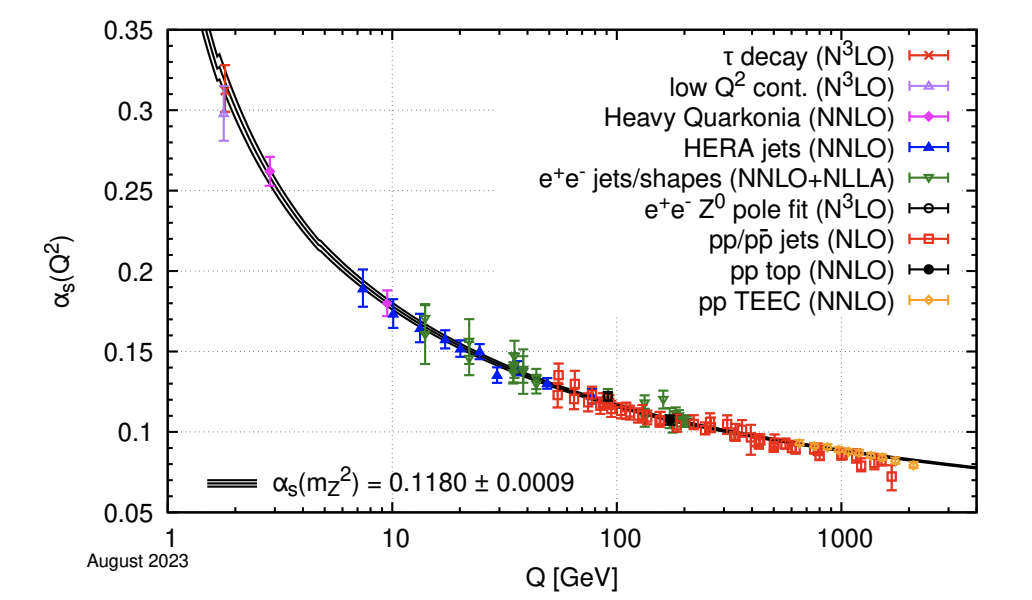
\includegraphics[keepaspectratio, scale=0.6]{fig/1_1_coupling_constant.png}
            \caption{QCD coupling constant\cite{ParticleDataGroup:2024cfk}}
            \label{coupling_constant}
        \end{figure}
        Figure \ref{coupling_constant} shows how the coupling constant $\alpha_s(Q^2)$ changes with the energy scale. The coupling constant becomes small at high energy scales, corresponding to short distances. This reflects the phenomenon of asymptotic freedom, where quarks behave as free particles when they are sufficiently close to each other. On the other hand, at low energy scales corresponding to long distances, the coupling constant grows infinitely large. This represents the phenomenon of quark confinement, where quarks cannot be isolated as individual particles.
        
        Next, I describe the self-interaction of gluons. The gluon field tensor is expressed as:
        \begin{eqnarray}
        \label{eq01}
            G^A_{\mu\nu} = \partial_\mu G^A_\nu - \partial_\nu G^A_\mu + g_s f^{ABC}G^B_\mu G^C_\nu
        \end{eqnarray}  
        where $f^{ABC}$ are the structure constants of the SU(3) group. Substituting this into the third term of (\ref{QCDlagrangian}), we obtain:  
        \begin{eqnarray}
            \nonumber
            -\frac{1}{4}G^A_{\mu\nu} G^{A\mu\nu} &=& -\frac{1}{4}(\partial_\mu G^A_\nu - \partial_\nu G^A_\mu + g_s f^{ABC} G^B_\mu G^C_\nu)(\partial^\mu G^{A\nu} - \partial^{\nu} G^{A\mu} + g_s f^{ABC} G^{B\mu} G^{C\nu})\\ 
            \nonumber
            &=& -\frac{1}{4}(\partial_\mu G^A_\nu - \partial_\nu G^A_\mu)(\partial^\mu G^{A\nu} - \partial^{\nu} G^{A\mu}) \\
            \label{selfinteraction}
            && \qquad\qquad\ - g_s f^{ABC}G^B_\mu G^C_\nu \partial^\mu G^{A\nu} - g_s^2 f^{ABE}f^{CDE}G^A_\mu G^B_\nu G^{C\mu}G^{D\nu}
        \end{eqnarray}  
        
        In (\ref{selfinteraction}), the first term represents the free gluon field without interactions. The second term represents interactions involving three gluon fields, representing reactions such as $g+g \rightarrow g$. The third term corresponds to interactions involving four gluon fields, representing reactions such as $g+g \rightarrow g+g$. For photons, the third term in \eqref{eq01} does not exist, so the second and third terms in (\ref{selfinteraction}) do not appear. This is because gluons interact with each other due to their color degrees of freedom, which gives rise to gluon self-interaction.  
        
        These characteristics—namely, the energy dependence of the coupling constant and the self-interaction of gluons—contribute to the complex structure of the quark-gluon interactions.
    \subsection{Chiral symmetry}
    \label{Intro:Chiral_symmetry}  
        The quark field can be separated into its right-handed and left-handed components. The projection operators for the right-handed and left-handed components are defined as $P_R$ and $P_L$, respectively. Using the $\gamma$ matrices, they are expressed as follows:  
        \begin{eqnarray}  
            P_R = \frac{1+\gamma_5}{2}, \quad P_L = \frac{1-\gamma_5}{2} 
        \end{eqnarray}  
        The following equations hold for these projection operators.
        \begin{equation}  
            P_R + P_L = 1, \quad P_R P_L = 0, \quad P_R^2 = P_R, \quad P_L^2 = P_L  
        \end{equation}  
        
        The right-handed quark field $q_R$ and the left-handed quark field $q_L$ are expressed using the projection operators as follows:  
        \begin{eqnarray}  
            q_R = P_R q, \quad q_L = P_L q
        \end{eqnarray}  
        
        These components are applied to the QCD Lagrangian:  
        \begin{eqnarray}  
            \mathcal{L}_{QCD} = \sum_q \bar{q}\qty(i\gamma^\mu D_\mu - m)q
        \end{eqnarray}  
        
        \begin{itemize}
            \item Kinetic Term (First Term of the QCD Lagrangian)
                    \begin{eqnarray}  
                        \bar{q}\qty(i\gamma^\mu D_\mu)q &=& \bar{q}\qty(i\gamma^\mu D_\mu)\qty(P_R^2 + P_L^2)q \\  
                        &=& \bar{q} P_L \qty(i\gamma^\mu D_\mu) P_R q + \bar{q} P_R \qty(i\gamma^\mu D_\mu) P_L q \\  
                        &=& \bar{q}_R \qty(i\gamma^\mu D_\mu) q_R + \bar{q}_L \qty(i\gamma^\mu D_\mu) q_L  
                    \end{eqnarray}  
            
            \item Mass Term (Second Term of the QCD Lagrangian)
                    \begin{eqnarray}  
                        \bar{q}m q &=& \bar{q} m \qty(P_R^2 + P_L^2)q \\  
                        &=& \bar{q} P_R m P_R q + \bar{q} P_L m P_L q \\  
                        &=& \bar{q}_L m q_R + \bar{q}_R m q_L
                    \end{eqnarray}  
        \end{itemize}
        
        From the above, the kinetic term of the quark field can be separated into the right-handed and left-handed quark fields, thereby preserving chiral symmetry. However, the mass term mixes the right-handed and left-handed quark fields, breaking chiral symmetry. Considering the chiral limit ($m_q = 0$), the QCD Lagrangian preserves chiral symmetry.  
        
        The order parameter for the spontaneous breaking of chiral symmetry is represented by the quark condensate $< \bar{q}q >$. As shown in Figure \ref{quark_condensate}, this quantity takes a finite value in the ground state of hadrons at standard temperature and density. But, it is expected to approach $< \bar{q}q > \sim 0$ at extremely high temperatures and densities.  
        \begin{figure}[htbp]  
            \centering  
            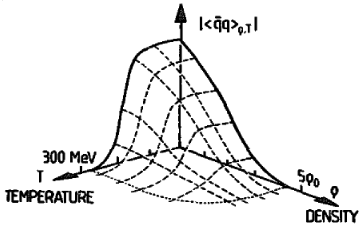
\includegraphics[keepaspectratio, scale=0.6]{fig/1_1_quark_condensate.png}  
            \caption{Quark condensate\cite{Weise:1993ax}}  
            \label{quark_condensate}  
        \end{figure}  
        
        Since the vacuum expectation value of the quark condensate cannot be directly measured, as described later, various other probes are used to investigate the restoration of chiral symmetry.
    \subsection{NJL model}
    \label{NJL model}      
        The interaction between quarks and gluons, as described in \ref{Intro:QCD}, exhibits a complex structure, making it difficult to understand various phenomena from first-principle calculations. Therefore, models are employed to describe various phenomena. One such model is the Nambu-Jona-Lasinio (NJL) model, a chiral effective model. Its Lagrangian is expressed as follows: 
        \begin{eqnarray}
            \label{NJLmodel}
            \mathcal{L}=\bar{q}i\gamma \cdot \partial q -(-g)\qty[(\bar{q}q)^2+(\bar{q}i\gamma_5q)^2]
        \end{eqnarray}  
        where, $q$ and $\bar{q}$ represent quark and antiquark fields, respectively; $\gamma$ and $\gamma_5$ are gamma matrices, with $\gamma_5 = i \gamma_0 \gamma_1 \gamma_2 \gamma_3$. Since there is an attractive force between quarks and antiquarks, the coupling constant $g$ is positive and has a dimension of $[\text{mass}]^{-2}$.  
        This model serves as a chiral effective theory for QCD at the energy scale of 1 GeV.\@ To determine the ground state of this Lagrangian, the self-consistent mean field approximation (MFA) is employed:  
        \begin{eqnarray}
            \label{sigma_ev}
            \ev{\bar{q}q}\equiv \frac{-m_0^2 \sigma}{G}\\
            \label{pi_ev}
            \ev{\bar{q}i\gamma_5q}\equiv \frac{-m_0^2 \pi}{G}
        \end{eqnarray}
        By substituting \eqref{sigma_ev} and \eqref{pi_ev} into \eqref{NJLmodel}, the expression is reformulated. Defining $\sigma = \bar{q}q$, $\pi = \bar{q} i \gamma_5 q$, and $2g = (G/m_0)^2$, we get:  
        \begin{eqnarray}
            \label{heikinbago}
            \mathcal{L}_{MFA} = \bar{q}\qty[i \gamma \cdot \partial - G(\sigma + i \pi \gamma_5)]q-\frac{m_0^2}{2}\qty(\sigma^2+\pi^2)
        \end{eqnarray}
        where, defining $q_\theta = e^{i \gamma_5 \frac{\theta}{2}} q$, $G \sqrt{\sigma^2 + \pi^2} = M$, and $\pi / \sigma = \tan{\theta}$, the Hamiltonian can be expressed as follows. $\theta$ is the parameter of the chiral transformation.  
        \begin{eqnarray}
            \label{ham}
            H_{MFA}=\int \dd[3]{\bm{x}}\qty{\bar{q}_\theta (x)(-i\gamma \cdot \nabla+M)q_{\theta}(x)+\frac{m_0^2}{2}\sigma_0^2}
        \end{eqnarray}
        where $\sigma_0^2 = \sigma^2 + \pi^2$. Since $\pi$ is considered sufficiently small, we write $\sigma$ to $\sigma_0$.  
        From this Hamiltonian, the Dirac equation for mass $M$ can be derived. Its solution is given as:  
        \begin{eqnarray}
            \label{Msol}
            q_\theta (x)=\frac{1}{\sqrt{V}}\sum_{\bm{p},r=\pm} \sqrt{\frac{M}{E_p}}\qty{a_M(\bm{p},r)u_M(\bm{p},r)e^{-ip\cdot x}+b_M^{\dag}(\bm{p},r)v_M(\bm{p},r)e^{ip\cdot x}}
        \end{eqnarray}
        where, $r$ represents helicity, $E_p = \sqrt{\bm{p}^2 + M^2}$, and $M = -g\ev{\bar{q}_\theta q_\theta}$.  
        Next, when $q_\theta(x)$ is expanded using spinors with zero mass, the solution is:  
        \begin{eqnarray}
            \label{0sol}
            q_\theta (x)=\frac{1}{\sqrt{V}}\sum_{\bm{p},s=R,L}\qty{a_{\bm{p}}^{(s)}(t)u_0(\bm{p},s)e^{-i\bm{p}\cdot \bm{x}}+b_{\bm{p}}^{(s)\dag}(t)v_0(\bm{p},s)e^{i\bm{p}\cdot \bm{x}}}
        \end{eqnarray}
        where $s$ represents helicity.  
        Using the solutions (\ref{Msol}) and (\ref{0sol}), the Hamiltonian (\ref{ham}) can be expressed in terms of operators for massive and massless states. Here, $a_{\bm{p}}$ and $b_{\bm{p}}$ are expansion coefficients:  
        \begin{align}
            %---------------------------------------------
            \label{hamenzan}
            H_{MFA}&=\sum_{\textbf{\textit{p}},s} \qty{|\textbf{\textit{p}}|(a_{\textbf{\textit{p}}}^{(s)\dag}(t) a_{\textbf{\textit{p}}}^{(s)}(t)-b_{-\textbf{\textit{p}}}^{(s)}(t)
            b_{-\textbf{\textit{p}}}^{(s)\dag}(t))+M\qty(b_{-\textbf{\textit{p}}}^{(s)} (t)a_{\textbf{\textit{p}}}^{(s)}(t)+a_{\textbf{\textit{p}}}^{(s)\dag}(t) b_{-\textbf{\textit{p}}}^{(s)\dag}(t))} +V \frac{m_0^2}{2}\sigma_0^2 \\
            %---------------------------------------------
            \label{massfinite}
            &=\sum_{\bm{p},r}E_p\qty(a^\dagger_M(\bm{p},r)a_M(\bm{p},r)-b_M(\bm{p},r)b^\dagger_M(\bm{p},r))+V\frac{m_o^2}{2}\sigma_0^2
            %---------------------------------------------
        \end{align}
        From this Hamiltonian, the following Heisenberg equation can be derived:  
        \begin{eqnarray}
            \label{massless_Heisenberg_e.q.}
            i \mqty(\dot{a}_{\textbf{\textit{p}}}^{(s)}(t)\\\dot{b}_{-\textbf{\textit{p}}}^{(s)}(t))=\mqty(|\textbf{\textit{p}}|&M\\M&-|\textbf{\textit{p}}|)\mqty(a_{\textbf{\textit{p}}}^{(s)}(t)\\b_{-\textbf{\textit{p}}}^{(s)}(t))
        \end{eqnarray}
        Setting the initial state $a_{\bm{p}}^{(s)}(t=0) = a_{M=0}(\bm{p},s)$, the solution reveals that the massive and massless operators are connected via the Bogoliubov transformation:  
        \begin{eqnarray}
            \label{Bogoliubov transformation}
            \mqty(a_{M}(\textbf{\textit{p}},r)\\b_{M}(\textbf{\textit{p}},r)^{\dag})=U(\textbf{\textit{p}},r) \mqty(a_0(\textbf{\textit{p}},r)\\b_0(\textbf{\textit{p}},r)^{\dag})U^{\dag}(\textbf{\textit{p}},r)
        \end{eqnarray}
        where $U(\bm{p},r) = \exp{-\frac{\theta_p}{2}(a_0^\dag(\bm{p},r)b_0^\dag(-\bm{p},r) - b_0(-\bm{p},r)a_0(\bm{p},r))}$.  
        The vacuum states for each operator are defined as follows:  
        \begin{eqnarray}
            \ket{\sigma_0} &\rightarrow&a_M(\textbf{\textit{p}},r)\ket{\sigma_0}=b_M(\textbf{\textit{p}},r)\ket{\sigma_0}=0\\
            \ket{0} &\rightarrow& a_0(\textbf{\textit{p}},r)\ket{0}=b_0(\textbf{\textit{p}},r)\ket{0}=0
        \end{eqnarray}
        
       $a_0(\textbf{\textit{p}},r)^{\dag}$ creates an eigenstate of chirality, while $a_M(\textbf{\textit{p}},r)^{\dag}$ creates an eigenstate of helicity. Based on the vacuum definition and \eqref{Bogoliubov transformation}, acting on $\ket{0}$ produces an eigenstate of helicity but not a definite chirality eigenstate. This implies that "chiral symmetry is spontaneously broken".  
        
        Thus, the NJL model theoretically predicts vacuum phase transitions. In our universe, it is believed that quark condensation spontaneously breaks chiral symmetry, leading to hadrons acquiring significant masses.
    \subsection{Quark-Gluon Plasma (QGP)}
        When hadrons are exposed to extremely high temperatures and densities, they transition into a plasma state known as the Quark-Gluon Plasma (QGP). In the QGP state, quarks are resolved from confinement, and the restoration of chiral symmetry is also expected. Furthermore, it is believed that the universe immediately following the Big Bang was in a QGP state. On the QCD phase diagram, which represents the phase structure of quarks and gluons, the QGP phase appears as shown in Figure \ref{QCD_Phase_Diagram}.  
        
        \begin{figure}[hbtp]
            \centering
            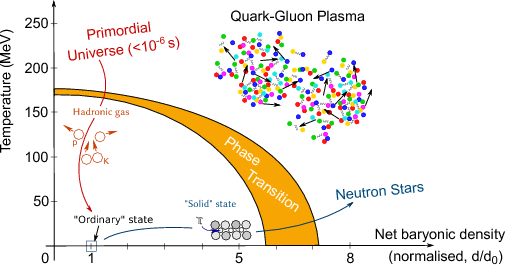
\includegraphics[keepaspectratio, scale=0.6]{fig/1_4_QCDPhaseDiagram.png}
            \caption{QCD Phase Diagram\cite{QCDPhaseDiagram}}
            \label{QCD_Phase_Diagram}
        \end{figure}
        The QGP phase can be observed in high-temperature regions in both high-density and low-density areas. Two types of phase transitions are related in the transition to the QGP phase. The first is the chiral phase transition. The second is the deconfinement-confinement phase transition.  
        
        The chiral phase transition is the spontaneous breaking of chiral symmetry as the vacuum undergoes a phase transition, allowing quarks to acquire a substantial effective mass. In other words, the chiral phase transition is deeply related to the mass acquisition of hadrons.  
               
        The deconfinement-confinement phase transition pertains to the confinement of quarks. In the hadronic ground state, quarks are confined by color interaction. However, in the QGP state, quarks are resolved from confinement and transition into a plasma state. This is the deconfinement-confinement phase transition. While these transitions are believed to occur at approximately a similar critical temperature, this relationship is not self-evident, and research is still ongoing. 
        
        % Additionally, an intriguing aspect of the QCD phase diagram is the nature of phase transition orders. At zero baryon number density, lattice QCD calculations have been extensively performed, revealing that the transition is a crossover, i.e., a continuous phase transition. On the other hand, in regions with high baryon number density, lattice QCD calculations face challenges due to the sign problem, making it difficult to predict the nature of the transition. Consequently, effective models play a crucial role. Analyses based on effective models suggest that a first-order phase transition is expected. Accordingly, research exploring the locations of phase transitions on the phase diagram remains highly active.  
    \subsection{Heaby Ion collision}
        The existence of QGP, which are ultrahigh-temperature or dense materials, has been confirmed by heavy-ion collision experiments. As shown in Figure  \ref{Intro:HIC:space_time_evaluation_of_HIC}, the time evolution proceeds in the following. 
        
        \begin{figure}[hbtp]
            \centering
            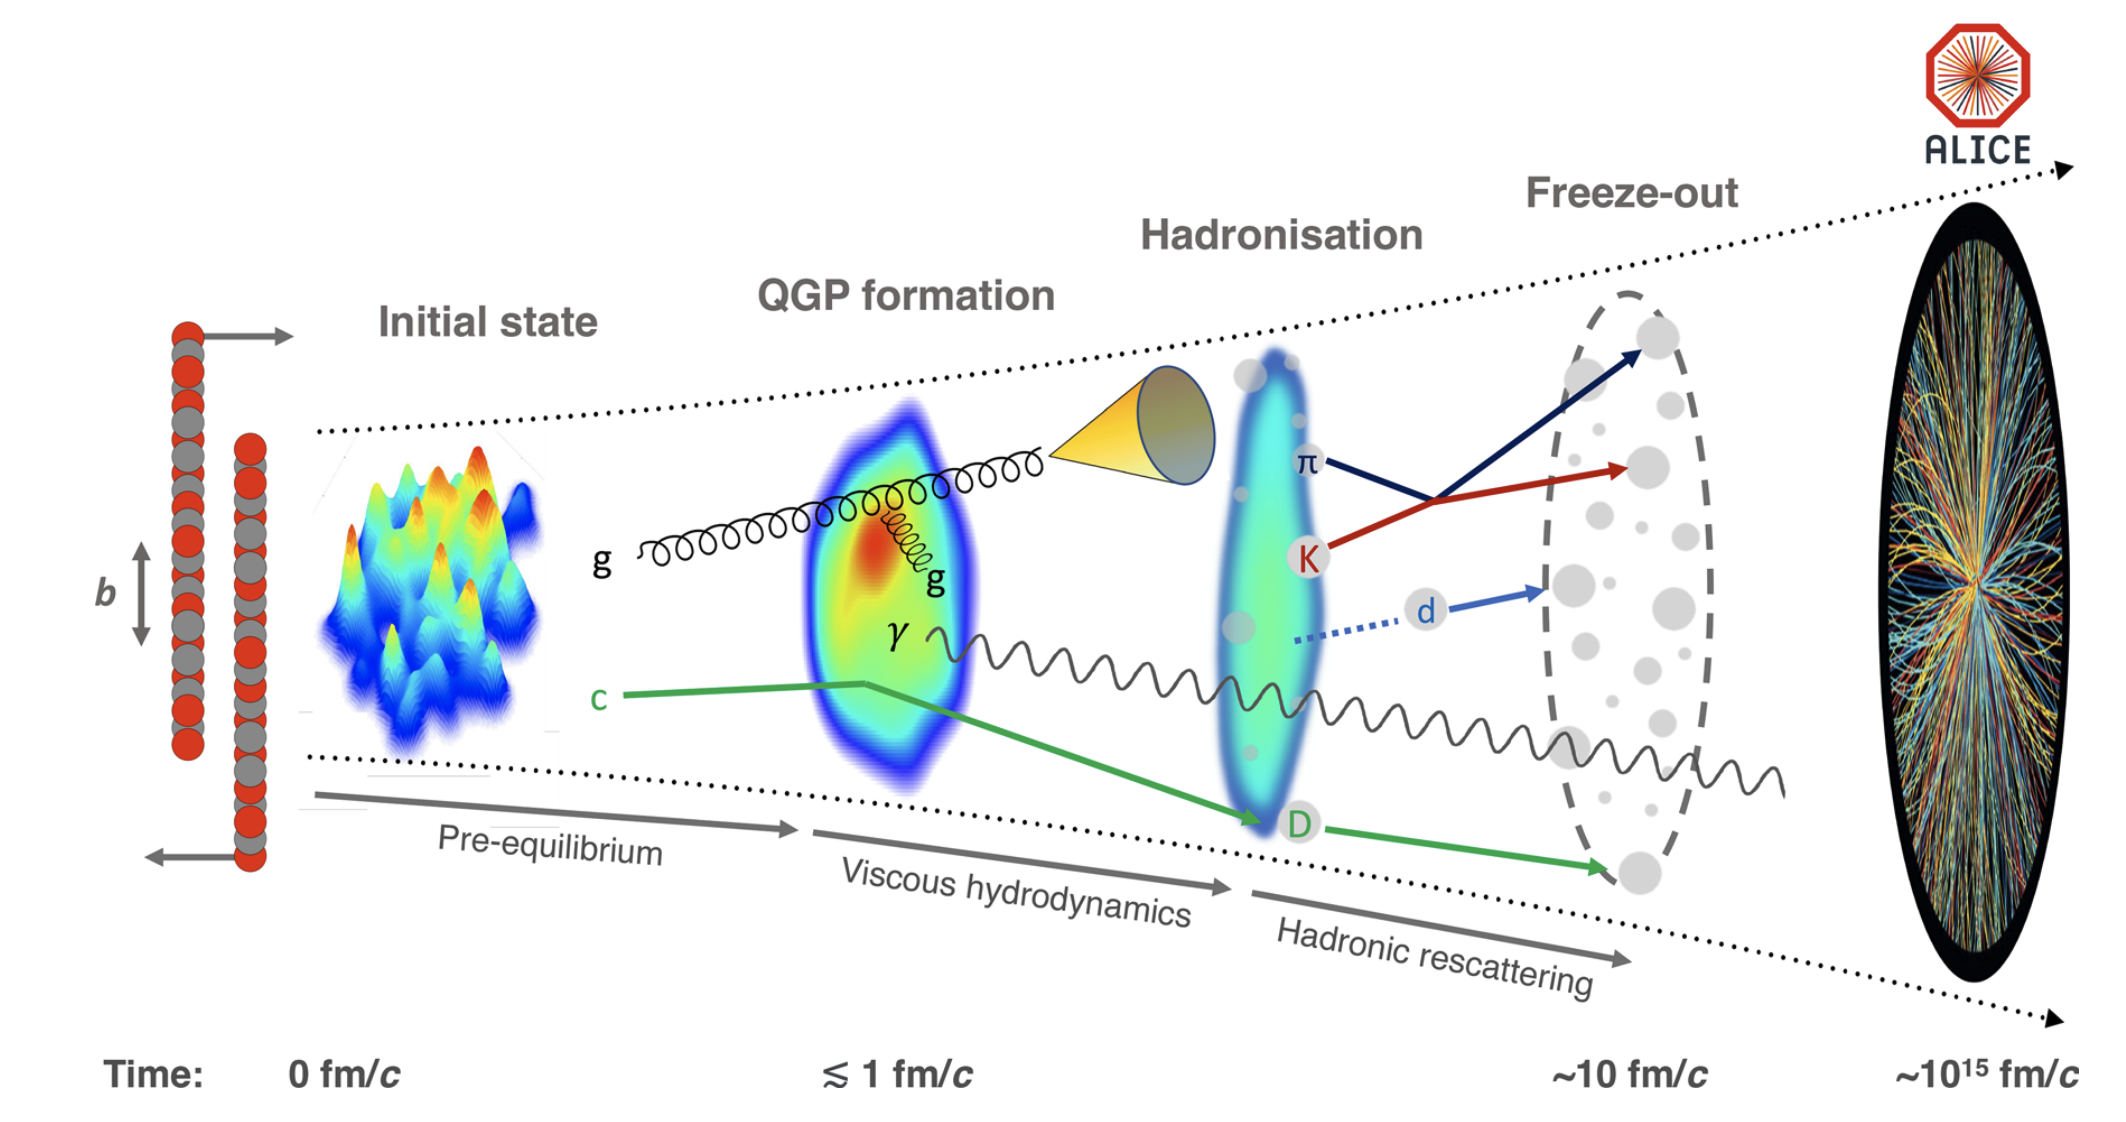
\includegraphics[keepaspectratio, scale=0.4]{fig/1_5_QGP_Evol.png}
            \caption{The evolution of a heavy-ion collision at LHC energies\cite{QGP_evo}}
            \label{Intro:HIC:space_time_evaluation_of_HIC}
        \end{figure}
        
        \begin{enumerate}
            \item Pre-equilibrium state
            \item QGP
            \item Hadronization
            \item Kinetic Freeze-out
        \end{enumerate}
        
        In the initial stage of the collision, partons from the nucleons undergo elastic and deep inelastic scatterings to reach thermalization. During this initial collision, phenomena such as jet production and the pair production of heavy quarks occur. Once the material generated in the collision region reaches thermal equilibrium, the system transitions into the QGP state.  
        
        In the QGP state, photons and lepton pairs originating from the thermal radiation of high-temperature matter are generated. Jets interact with the QGP and lose energy, resulting in jet quenching, while heavy quarks undergo deconfinement due to the color Debye screening. Subsequently, as the QGP cools, hadronization occurs, leading to chemical freeze-out.  
        
        Chemical freeze-out refers to the stop of changes in particle species due to deeply inelastic scatterings among particles. However, elastic scatterings between hadrons continue, and momentum exchange among particles. Later, kinetic freeze-out occurs, fixing the momenta and other properties of the particles. The particles finally detected are those that remain after the kinetic freeze-out. Thus, QGP is formed during the temporal evolution of heavy-ion collisions, and its lifetime is extremely short. 
        
        % Here, since partons strongly interact with the QGP, only the final state of heavy-ion collisions is observed. However, leptons and photons do not undergo strong interactions, so their measurements reflect the integration over the entire temporal evolution.
        
        % Some evidence of QGP includes jet quenching and strong elliptic flow. Jet quenching refers to the phenomenon where high-energy partons produced during the initial stage of high-energy collisions generate numerous high-momentum particles along their flight direction. However, due to their interactions with the QGP, the jets are quenched. High-energy partons passing through the medium lose energy, suppressing the jet phenomenon. Additionally, strong elliptic flow occurs when QGP generated during heavy-ion collisions exhibits a distinct collective flow depending on its density and temperature.
        
        The QGP generated in heavy-ion collisions has its density and temperature determined by the collision energy. High-density QGP regions are realized at collision energies of $\sqrt{s_{NN}} \lesssim 10$ [GeV].\@ At these energies, the colliding particles stop at the collision point. They create a high-density state where kinetic energy is converted directly into heat, increasing the temperature.  
  
        On the other hand, high-temperature, low-density regions are achieved at collision energies of $\sqrt{s_{NN}} \gtrsim 100$ [GeV].\@ In this energy regime, the colliding particles do not stop but pass through each other, producing a large number of pair creation. As a result, the baryon number density does not become large relative to the temperature. However, a high energy density region leads to the creation of high-temperature matter near the collision point.  
        
        In the ALICE experiment, LHC Run 3 operations began in 2022, initiating Pb-Pb collision measurements at $\sqrt{s_{NN}} = 5.36$ TeV.\@ This collision energy produces QGP in the ultrahigh temperature, low-density region. Moreover, compared to the QGP generated at $\sqrt{s_{NN}} = 200$ GeV at RHIC, the higher collision energy at LHC enables the measurement of a larger QGP than ever before.

    \subsection{Dilepton Measurement\cite{Geurts:2022xmk}}
        Dilepton measurement is a good probe to investigate the time evolution of heavy-ion collisions. Leptons do not interact with strong interactions, making them less affected by the QGP.\@ This characteristic allows for the measurement of a distribution that sums up dileptons from all stages of heavy-ion collisions. The sources of dilepton production are as follows:   
        
        \begin{figure}[hbtp]
            \centering
            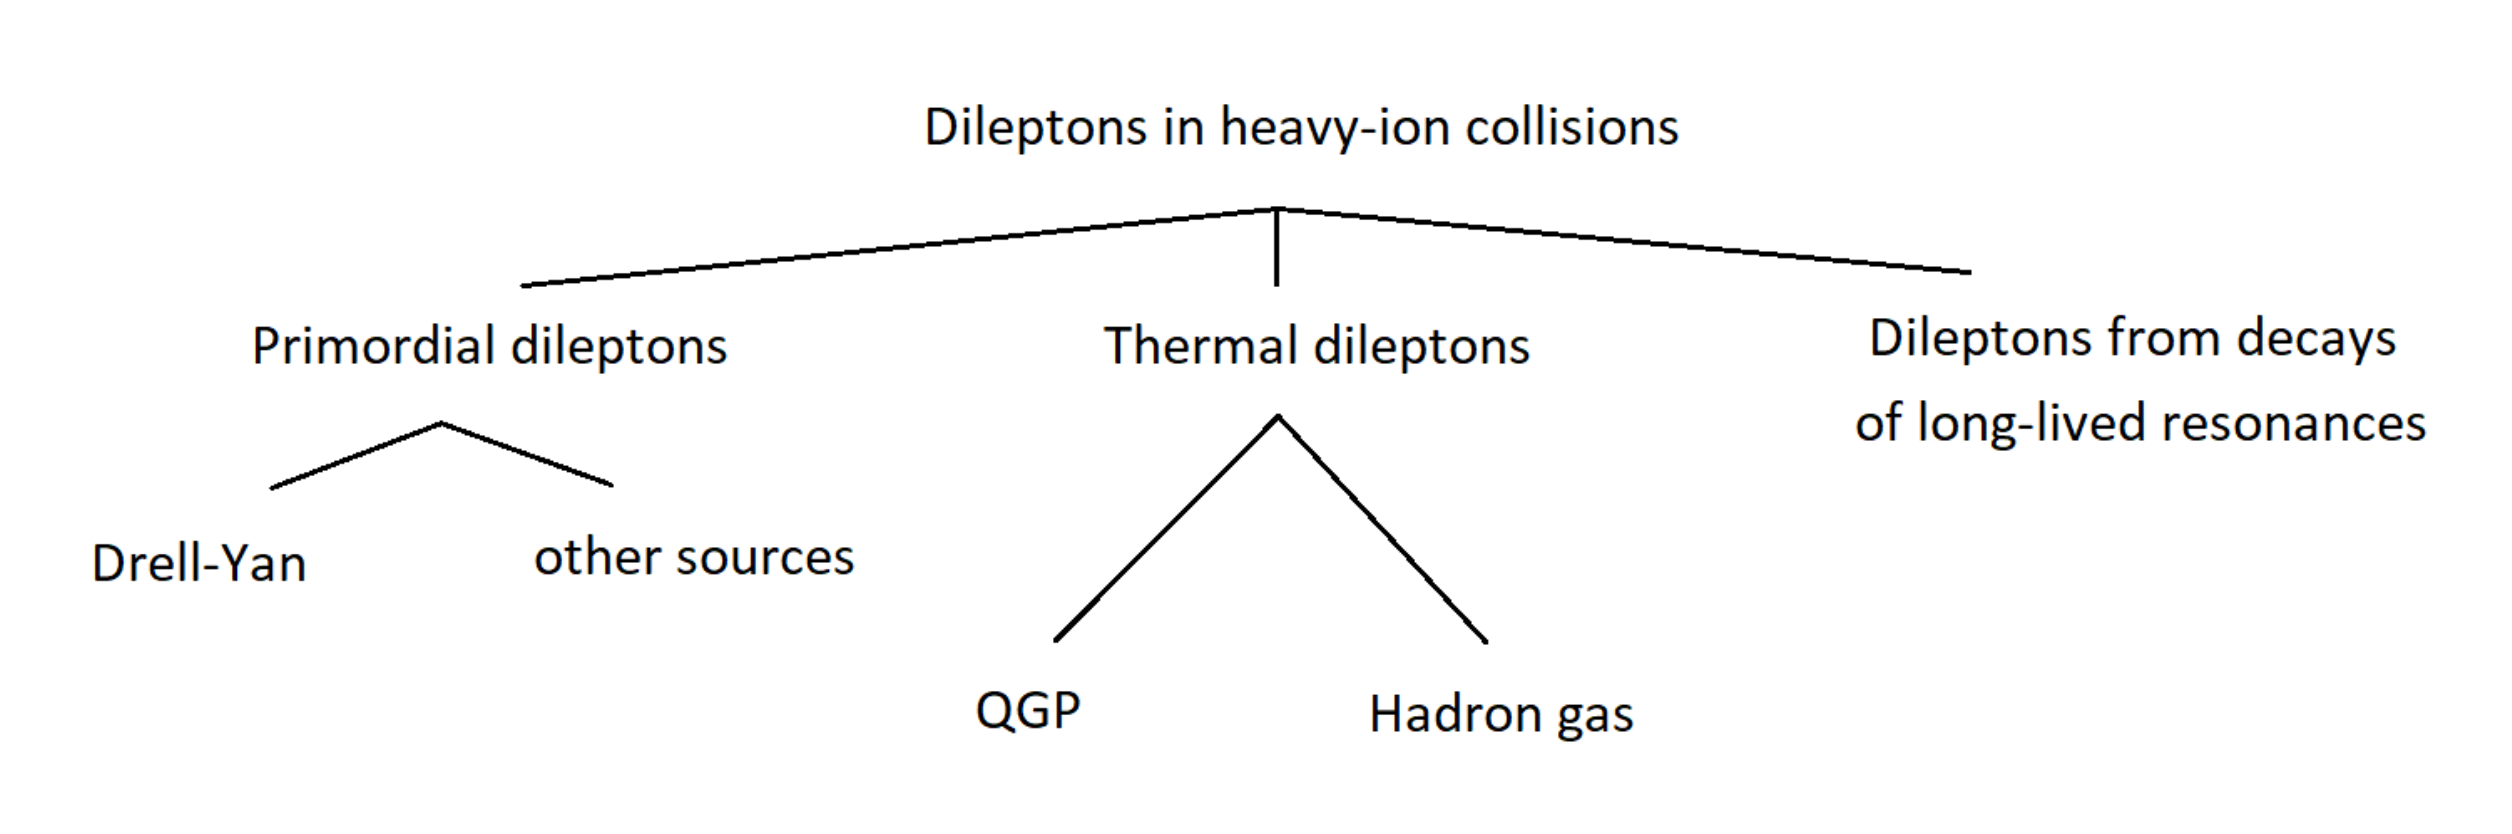
\includegraphics[keepaspectratio, scale=0.3]{fig/1_5_dilepton_source.png}
            \caption{Dilepton source}
            \label{Intro:Dilepton:dilepton_source}
        \end{figure}
        
        \begin{itemize}
            \item Primordial dileptons (from \(q\bar{q}\) annihilation)
            \item Thermal dileptons
            \item Dileptons from hadron decays
        \end{itemize} 
        The dilepton mass regions are associated with the time evolution of heavy ion collisions respectively.
        \begin{figure}[hbtp]
            \centering
            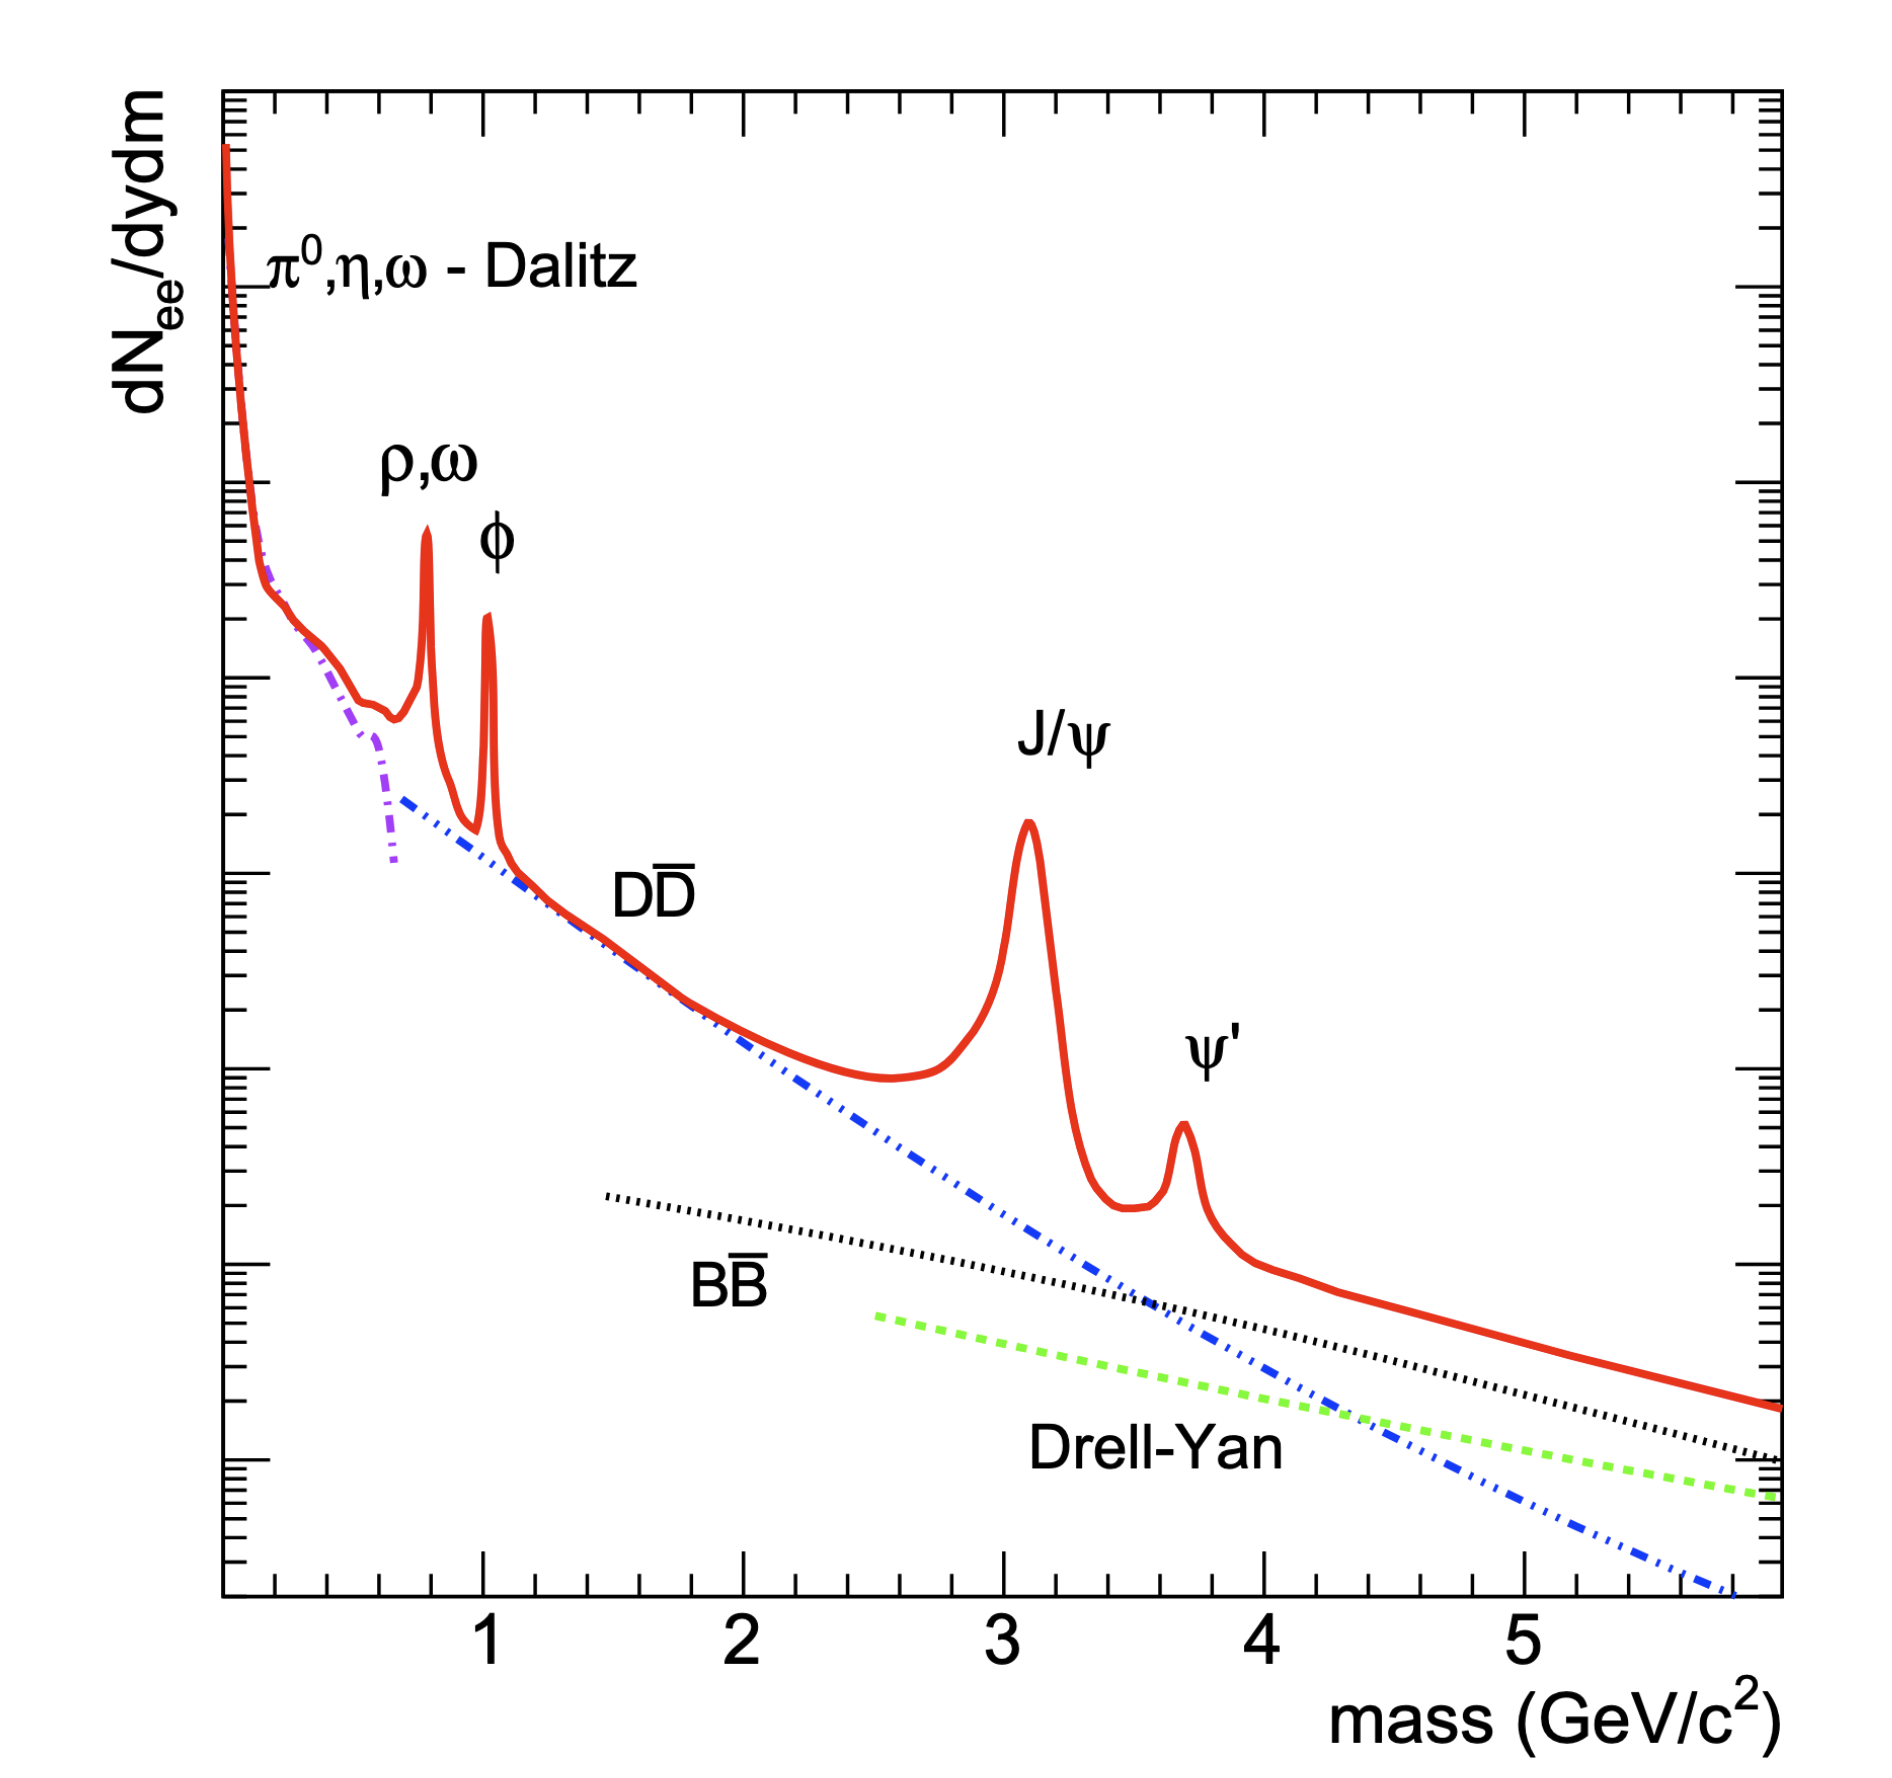
\includegraphics[keepaspectratio, scale=0.3]{fig/1_6_expected_dileptonMass.png}
            \caption{Expected mass spectrum from dileptons\cite{Rapp:1999ej}}
            \label{Intro:Dilepton:dilepton_mass}
        \end{figure}
        
        In the High-Mass Region, primordial dileptons (Drell-Yan) constitute the continuum component of the mass distribution. It is related to the initial state of the collision. In the Intermediate-Mass Region, thermal dileptons originating from the QGP and continuum components such as open-charm and open-beauty are observed. 
        
        Finally, in the Low-Mass Region, the dilepton distribution is predominantly derived from light meson decays from the hadronic gas. Most dileptons from hadron decays have longer lifetimes compared to the QGP.\@ So these mesons observed in this region are mostly from the hadron gas. However, light vector mesons $(\rho, \omega, \phi)$ have extremely short lifetimes. They may be affected by QGP.\@
    \subsection{Search for chiral symmetry restoration in QGP}
        \begin{figure}[hbtp]
            \centering
            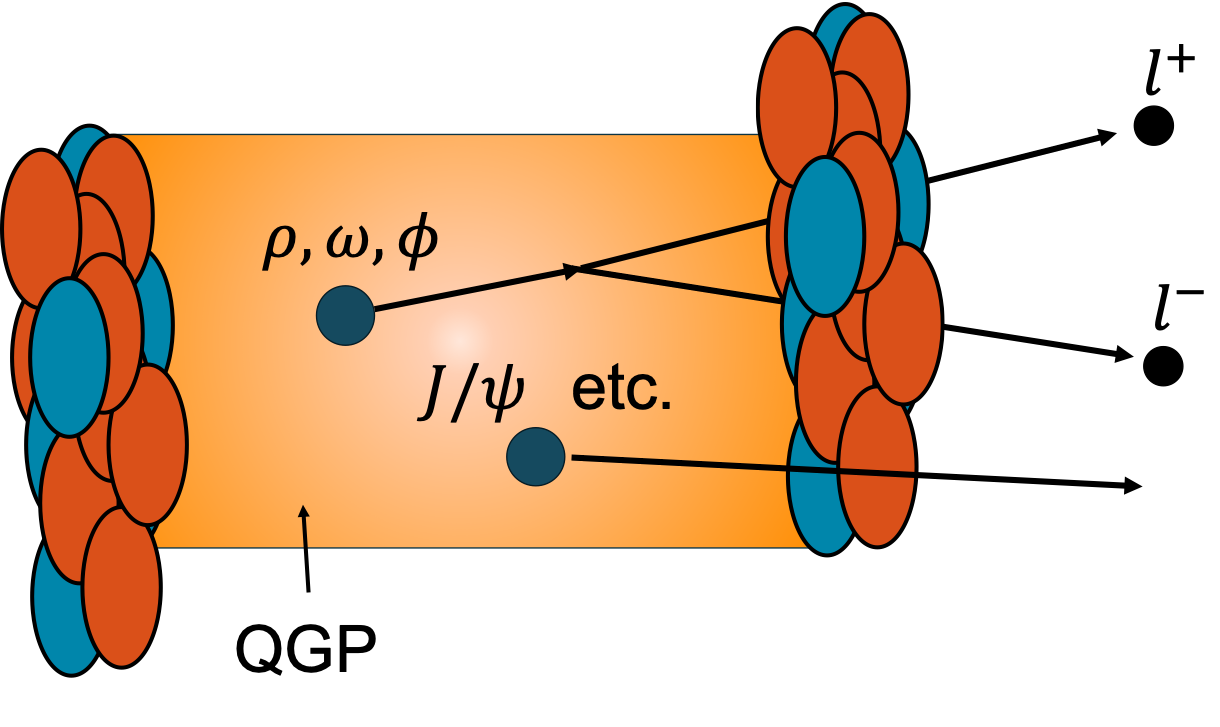
\includegraphics[keepaspectratio, scale=0.2]{fig/1_7_Search_for_chiral.png}
            \caption{Low mass vector meson decay in QGP}
            \label{Intro:Search_for_CSR:Low_mass_vector_meson_decay_in_QGP}
        \end{figure}
        
        In the QGP, it is expected that an ultra-high temperature and high-density state is realized, leading to $ < \bar{q}q > \sim 0 $ and the restoration of chiral symmetry. Light vector mesons $(\rho, \omega, \phi)$ serve as probes for the masses of hadrons in the QGP.\@ These particles have short lifetimes and decay channels into dileptons. As shown in Fig.4, their short lifetimes make it possible for them to decay within the QGP, which would otherwise immediately hadronize. Additionally, since they decay exclusively into dileptons, which do not undergo strong interactions with the QGP, the masses of hadrons within the QGP can be measured.  
        
        In past experiments, the restoration of chiral symmetry was investigated using dileptons. In the SPS-NA60 experiment, the excess of muon pairs in the low-mass region was reported. However, the excess could also be explained by $\pi + \pi \rightarrow \rho \rightarrow \pi \pi$, and thus it did not serve as definitive evidence of chiral symmetry restoration\cite{NA60}.  
        
        Additionally, in the electron pair measurements during ALICE Run 2 $\sqrt{s_{NN}} = 5.02$ TeV PbPb collisions, contributions from open-charm and open-beauty were estimated along with the vacuum dilepton distribution excluding $\rho$, and an excess of electron pairs was reported.the excess was explained as thermal dileptons from the QGP within the error range.demonstrated\cite{ALICE:2023jef}.  
        
        This study aims to measure the mass modification of light vector mesons in the QGP using forward muon pairs in ALICE Run 3 $\sqrt{s_{NN}} = 5.36$ TeV PbPb collisions. Starting from ALICE Run 3, the MFT was introduced into the forward detector system of the ALICE experiment. It enables more precise measurements of muon production points compared to Run 2, as well as measurements of muons with lower transverse momentum. By utilizing the differences in muon production points of heavy flavor (HF), which is one of the backgrounds in light vector meson measurements, can be removed. This will allow the precise measurement of the mass distribution of low transverse momentum light vector mesons, which are more likely to decay within the QGP.\@
    \subsection{Analysis of pp collision data as a baseline}
    This paper presents the analysis results of proton-proton collision events. The particles generated in proton-proton collisions are produced from the vacuum. Measurements of collision events where QGP is not produced serve as a baseline for comparison with events where QGP is generated. Currently, the quality of track reconstruction is still insufficient, and the muon pair analysis is also incomplete. Furthermore, the quality of muon tracks in heavy-ion collisions is more challenging than in proton-proton collisions due to the large number of particles generated in each event.  

    The purpose of this study is to provide an analysis as a baseline for future studies of $\sqrt{s_{NN}} = 5.02$ PbPb collisions, where QGP is expected to be generated and to improve the quality of muon tracks in ALICE Run 3 $\sqrt{s_{NN}} = 13.6$ TeV pp collisions.

    %第2章
    \section{Detector setup}
    \subsection{LHC-ALICE}
    \begin{figure}[htbp]
        \centering
        \includegraphics[keepaspectratio, scale=0.2]{fig/ALICE_RUN3_detectors.jpg}
        \caption{ALICE detectors}
        \label{ALICE_detectors}
    \end{figure}
    \subsection{Barrel detectors}
    \subsection{Forward detectors}
    \begin{figure}[htbp]
        \centering
        \includegraphics[keepaspectratio, scale=0.7]{fig/muon_detectors.png}
        \caption{MFT-MCH-MID}
        \label{muon_detectors}
    \end{figure}
    \subsection{Track reconstruction}


    %第3章
    \section{Analysis}
\label{Analysis}
    \subsection{DataSet}
    \label{DataSet}
        The data used is a part of $pp$ collisions at $\sqrt{s}=13.6$ TeV obtained in 2022. The collision rate of $pp$ is $500$ kHz, and the dataset name is LHC22o$\_$apass7.
        The Monte Carlo simulation data used in \ref{Analysis:Matching} utilized Pythia8 Monash to reproduce 500 kHz $pp$ collisions at $\sqrt{s}=13.6$ TeV, employing minimum bias event simulations without extracting specific events.
        
    \subsection{Event selection}
    \label{Event_selection}
        The ITS detector system measured the position of the proton-proton collision. The Z-coordinate of the collision point, denoted as VtxZ, was selected with the condition $|VtxZ| < 10$ cm, using the ITS centre at Z = 0 as the reference. This cut value is adjusted with the ITS acceptance. The number of events obtained with this cut is $5.5 \times 10^9$.\@

    \subsection{Single muon track reconstruction}
    \label{Single_reco}
        The Global track reconstructed in \ref{MFT-MUON_matching} was used to calculate the physical quantities of the muon as follows. The MFT standalone Track measures the muon's $\eta$ and $\phi$. The momentum $p$ was derived by propagating the MCH standalone track to the Z-coordinate of the collision point, with corrections applied for multiple scattering and energy loss in the absorber.
        For the DCA, a global fit was performed for all tracks constituting the Global Track, and the resulting track was used. 
        As shown in Fig. \ref{Analysis:reco:DCA}, the track was linearly extrapolated to the Z-coordinate of the collision point (IP), and the distance between the extrapolated point and the collision point was calculated as the DCA. Similarly, using the same track, $R_{abs}$ was calculated as the distance from the beam axis at the back edge of the absorber, as shown in Fig. \ref{Analysis:reco:R_abs}.\@
        Furthermore, the MFT-MCH matching $\chi^2$ was calculated based on the parameter differences when extrapolating the MFT track and MCH track to the matching plane.
        \begin{figure}[htbp]
            % Left figure
            \begin{minipage}{0.45\textwidth} % Specifying the width with minipage
                \centering
                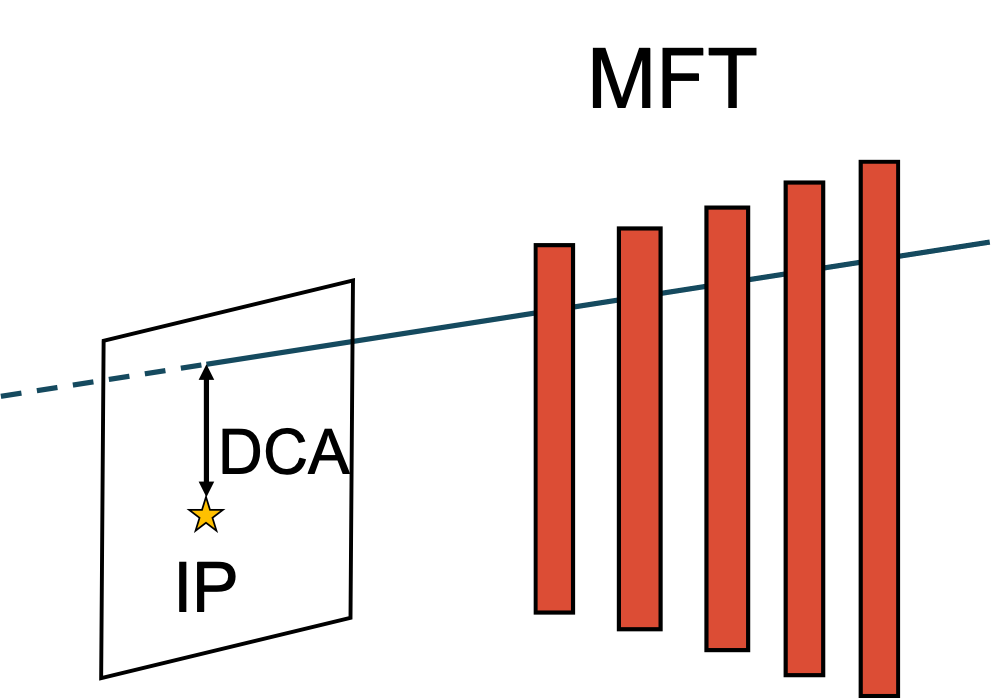
\includegraphics[keepaspectratio, scale=0.15]{fig/3_3_DCA.png} % Left image
                \caption{conceptual scheme of DCA}
                \label{Analysis:reco:DCA}
            \end{minipage}
            % Right figure
            \hspace{0.5cm}
            \begin{minipage}{0.45\textwidth}
                \centering
                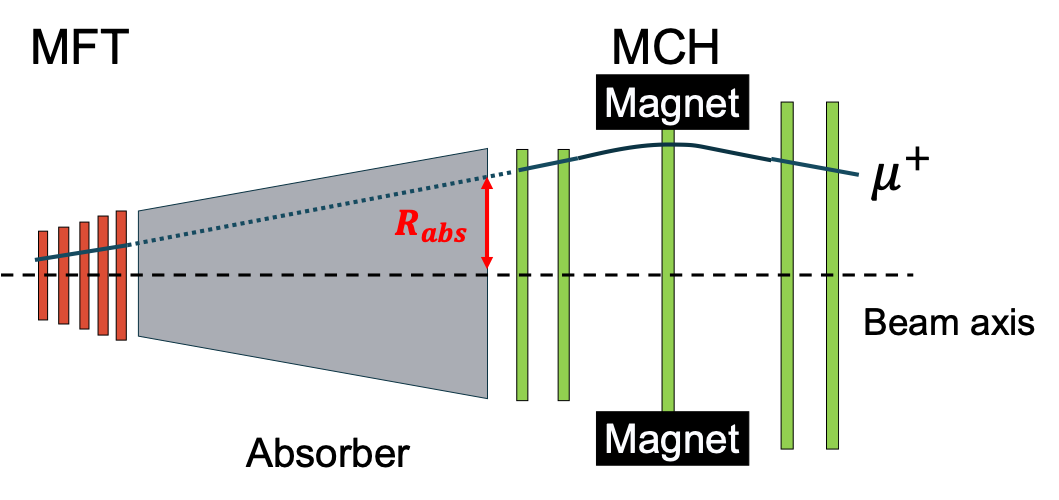
\includegraphics[keepaspectratio, scale=0.15]{fig/3_3_Rabs.png} % Right image
                \caption{conceptual scheme of $R_{abs}$}
                \label{Analysis:reco:R_abs}
            \end{minipage}
        \end{figure}

    \subsection{Single muon selection}
    \label{Single_muon_selection}
        The cuts applied to the obtained muon tracks are as follows:
        \begin{itemize}{}
            \item -3.6 <$\eta$ < -2.5
            \item 17.5 cm < $R_{abs}$ < 89.5 cm
            \item $pDCA$ < 6$\sigma$
            \item MFT-MCH matching $\chi^2$ < 30
        \end{itemize}
        The $\eta$ cut is adjusted to match the MFT-MHC-MID acceptance. 
        The cut value of $R_{abs}$ removes tracks of values where hadron absorbers are not present.
        The pDCA is the momentum multiplied by DCA, and this cut value removes muons derived from the beam gas. The cut was applied at 6$sigma$ when Gaussian-fitted to the pDCA distribution.
        MFT-MCH matching $\chi^2$ values, optimised to a value that maximises the statistical error of the $\omega,\phi$ yield as described below.
        The final MFT-MCH matching $chi^2$ values are obtained from a fit using the points detected when matching MFT and MCH tracks. The values used in this study are optimised to minimise the statistical uncertainty in the $omega$ and $phi$ yields, as discussed below.
    
        \subsection{Dimuon analysis}
        \label{Dimuon}
            \subsubsection{Dimuon reconstruction}
            \label{Dimuon_reco}
                Dimuons are reconstructed using the single muons selected in \ref{Single_muon_selection}. The mass($M_{\mu\mu}$), transverse momentum($p_T$), pseudorapidity($\eta$), and Azimuth angle($\phi$) of the dimuon are calculated as (\ref{px})~(\ref{eta_mumu}). First, the $p_T$, $\eta$, and $\phi$ of the single muons are converted into four-component vectors $(p_x, p_y, p_z, E)$ using (\ref{px}),(\ref{py}),(\ref{pz}),(\ref{E}).\@
                \begin{eqnarray}
                    p_x &=& p_T \cos(\phi)\\ \label{px}
                    p_y &=& p_T \sin (\phi)\\ \label{py}
                    p_z &=& p_T \sinh (\eta)\\ \label{pz}
                    E &=& \sqrt{p_T^2 \cosh^2(\eta) + m_\mu^2} \label{E} 
                \end{eqnarray}
                Then, using the $(p_x, p_y, p_z, E)$ of the single muons, the $(P_x, P_y, P_z, E_{\mu\mu})$ of the dimuon are calculated.
                \begin{eqnarray}
                    \begin{pmatrix}
                        P_x \\
                        P_y \\
                        P_z \\
                        E
                    \end{pmatrix}
                    &=&
                    \begin{pmatrix}
                        p_{x1} \\
                        p_{y1} \\
                        p_{z1} \\
                        E_1
                    \end{pmatrix}
                    +
                    \begin{pmatrix}
                        p_{x2} \\
                        p_{y2} \\
                        p_{z2} \\
                        E_2
                    \end{pmatrix}
                \end{eqnarray}
                Using the obtained four-component vector of the dimuon $(Px, Py, Pz, E_{\mu\mu})$, the pair's $M_\mu\mu$, $p_T$, and $\eta$ were calculated from the (\ref{M_mumu}),(\ref{pT_mumu}),(\ref{eta_mumu}).
                \begin{eqnarray}
                    M_{\mu\mu} &=& \sqrt{E^2 - (p_x^2 + p_y^2 + p_z^2)}\\ \label{M_mumu}
                    p_{T\mu\mu} &=& \sqrt{p_x^2 + p_y^2}\\ \label{pT_mumu}
                    \eta_{\mu\mu} &=& -\log\left(\tan\left(\frac{1}{2}\arctan\left(\frac{\sqrt{p_x^2 + p_y^2}}{p_z}\right)\right)\right) \label{eta_mumu}
                \end{eqnarray}
                Using (\ref{M_mumu}),(\ref{E_mumu}) and (\ref{eta_mumu}), the physical quantities of the dimuon are calculated.
                
            \subsubsection{Combinatorial background subtraction}
            \label{Analysis:Dimuon:Combinatorial BG subtraction}
                The dimuon was reconstructed by pairing oppositely charged muons present in each event. In cases with multiple combinations, all combinations are used to pair the muons and reconstruct the physical quantities of the dimuon. Since all combinations are considered, the mass distribution of uncorrelated muon pairs is also reconstructed. This is called the combinatorial background. This study uses the Like Sign method to subtract the combinatorial background. The Like Sign method is a method that estimates the combinatorial background by using the mass distribution of muon pairs with the same sign from each collision event. The key feature of this method is that it estimates the shape of uncorrelated background events using the like-sign muons from the same event, allowing for the subtraction of mass distributions of weakly correlated particles within each event, such as those arising from elliptic flow in heavy-ion collisions. The estimated uncorrelated background events depend on the $p_T$ of the dimuon.
                The calculation formula is given by (\ref{LikeSignMethod}).
                \begin{eqnarray}
                    \label{LikeSignMethod}
                    \dv{N_{sig}}{m} &=& \dv{N_{same}^{+-}}{m} - 2R \sqrt{\dv{N_{same}^{++}}{m} \dv{N_{same}^{--}}{m}}\\
                    2R &=& \frac{\dv{N_{mix}^{+-}}{m}}{\sqrt{\dv{N_{mix}^{++}}{m} \dv{N_{mix}^{--}}{m}}} 
                \end{eqnarray}
                Where, $\dv{N_{sig}}{m}$ represents the number of correlated muons at each mass, $\dv{N_{same}^{**}}{m}$ represents the number of same-sign muon pairs in the same event (** corresponds to the muon sign), and $\dv{N_{mix}^{**}}{m}$ represents the number of muon pairs formed from different events. R is a term to correct for the acceptance difference due to the muon sign. R=1 when there is no difference in acceptances by sign. Since muon pairs from different events were not reconstructed in this analysis, R = 1 was used for the calculation.

                The result of the combinatorial background subtraction in the dimuon transverse momentum region of (1 < $p_T$ < 30) GeV is shown in Figure \ref{All_pt_CB}.
                \begin{figure}[H]
                    \centering
                    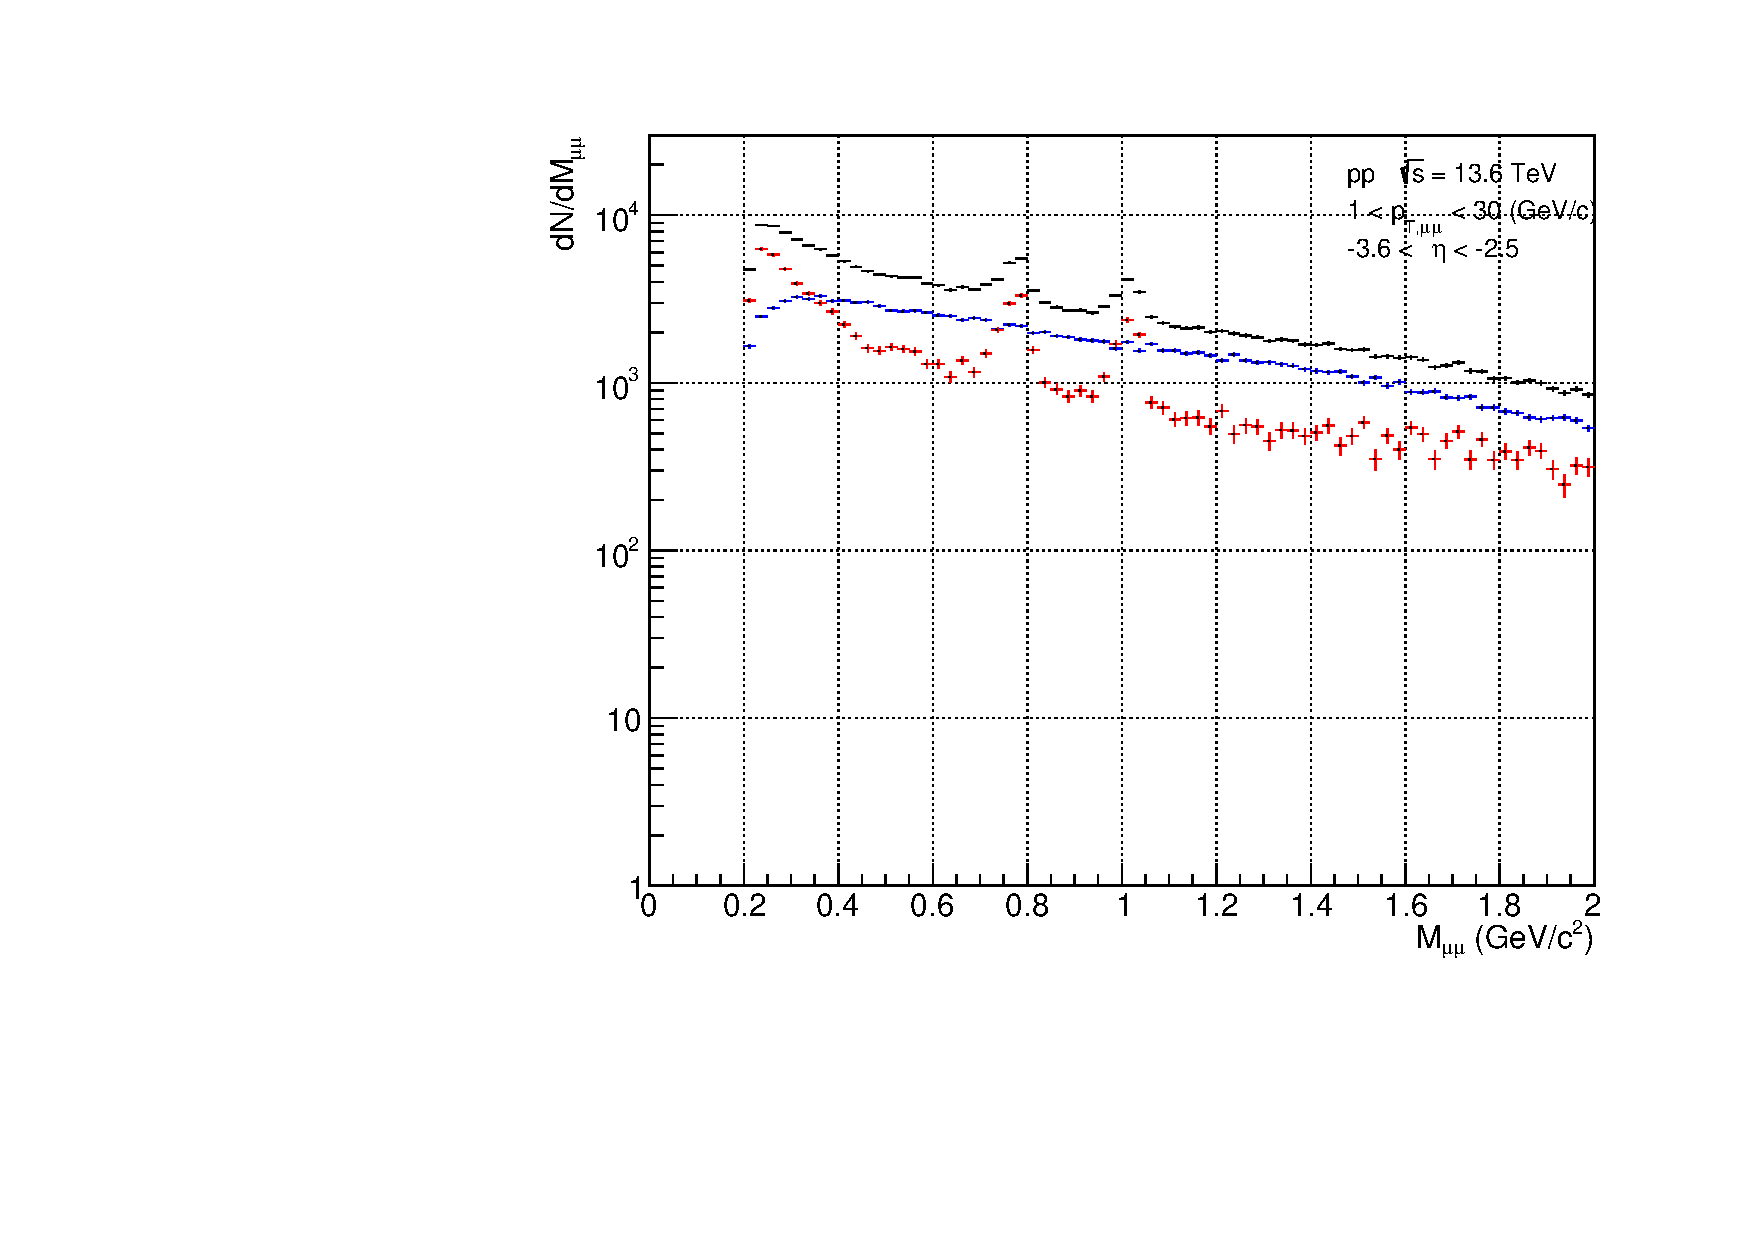
\includegraphics[keepaspectratio, scale=0.5]{fig/3_4_1_CB_pt_1to30.pdf}
                    \caption{1 < $p_{T}$ < 30}
                    \label{All_pt_CB}
                \end{figure}
                The black distribution represents the invariant mass reconstructed by pairing oppositely charged muon particles from all combinations within the same event, while the blue distribution represents the uncorrelated background events estimated using the Like Sign method. The red distribution, obtained by subtracting the blue from the black one, represents the dimuon invariant mass distribution with correlations.
                The mass distributions were separated by dimuon $p_T$, and uncorrelated background events were subtracted using the Like Sign method in each invariant mass distribution to examine the transverse momentum dependence of the $\omega$ and $\phi$ yields. The subtracted plots are shown in Figure \ref{Analysis:Dimuon:CB:CB_pt_separation}.

                \begin{figure}[H]
                    \centering
                    \begin{minipage}{0.45\textwidth}
                        \centering
                        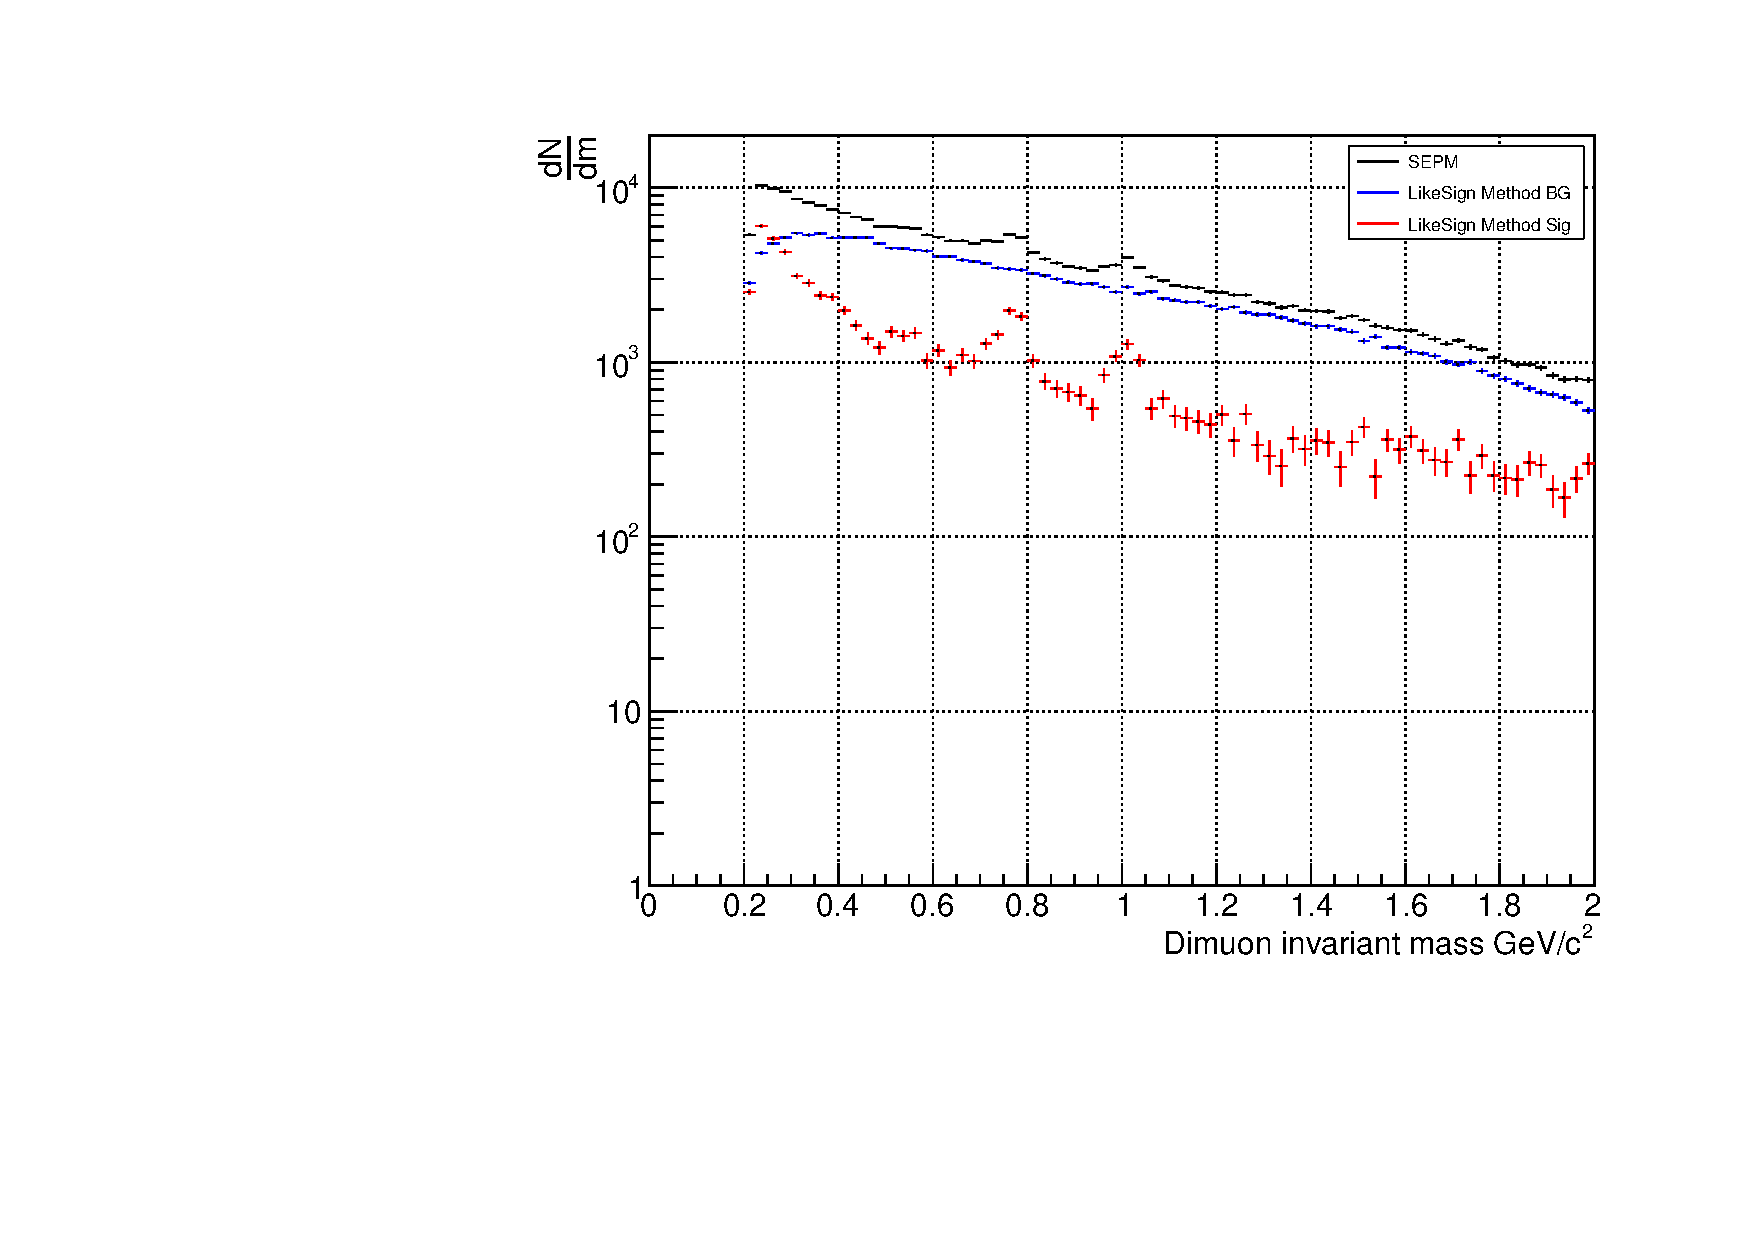
\includegraphics[width=\textwidth]{fig/3_4_1_CB_pt_1to2.pdf}
                        \caption*{1 < $p_{T}$ < 2}
                    \end{minipage}
                    \hfill
                    \begin{minipage}{0.45\textwidth}
                        \centering
                        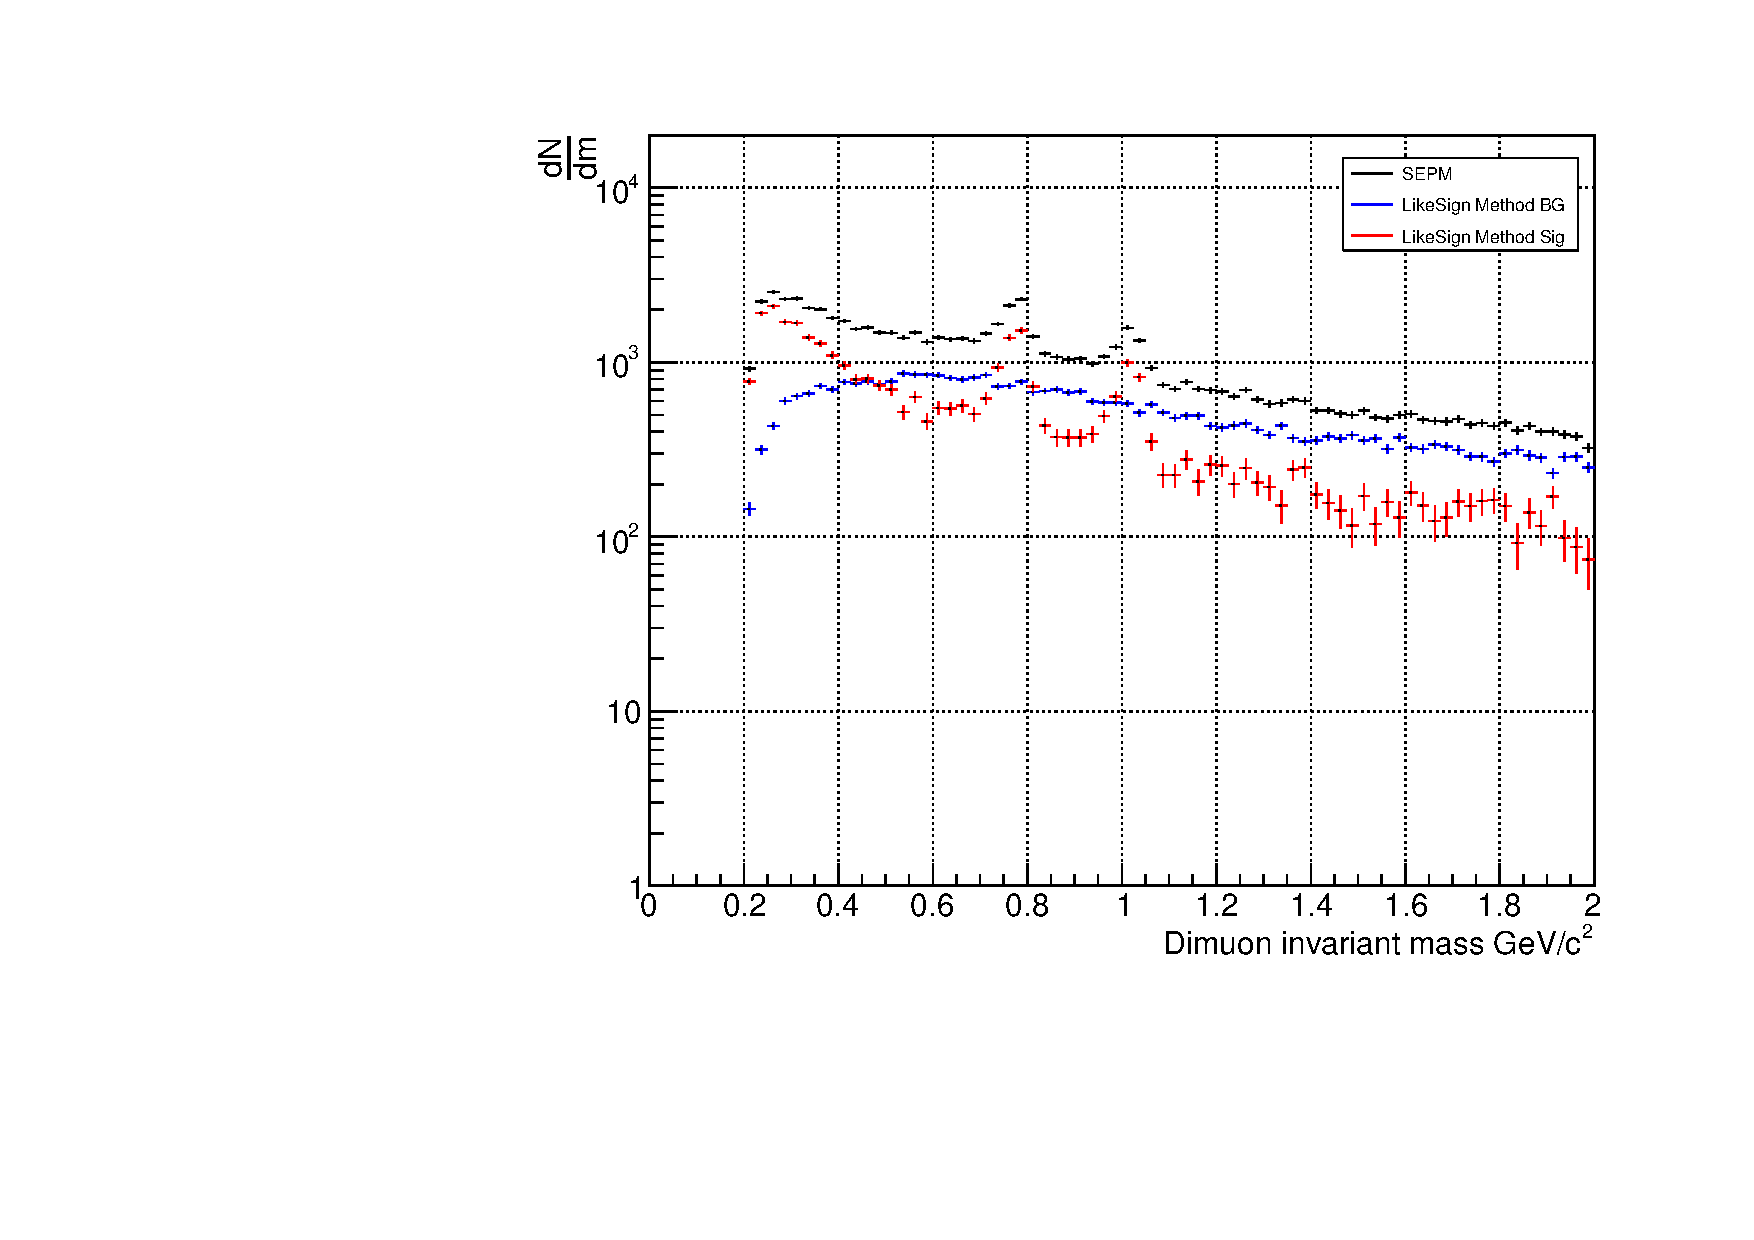
\includegraphics[width=\textwidth]{fig/3_4_1_CB_pt_2to3.pdf}
                        \caption*{2 < $p_{T}$ < 3}
                    \end{minipage}
                    \\
                    \vspace{1em}
                    \begin{minipage}{0.45\textwidth}
                        \centering
                        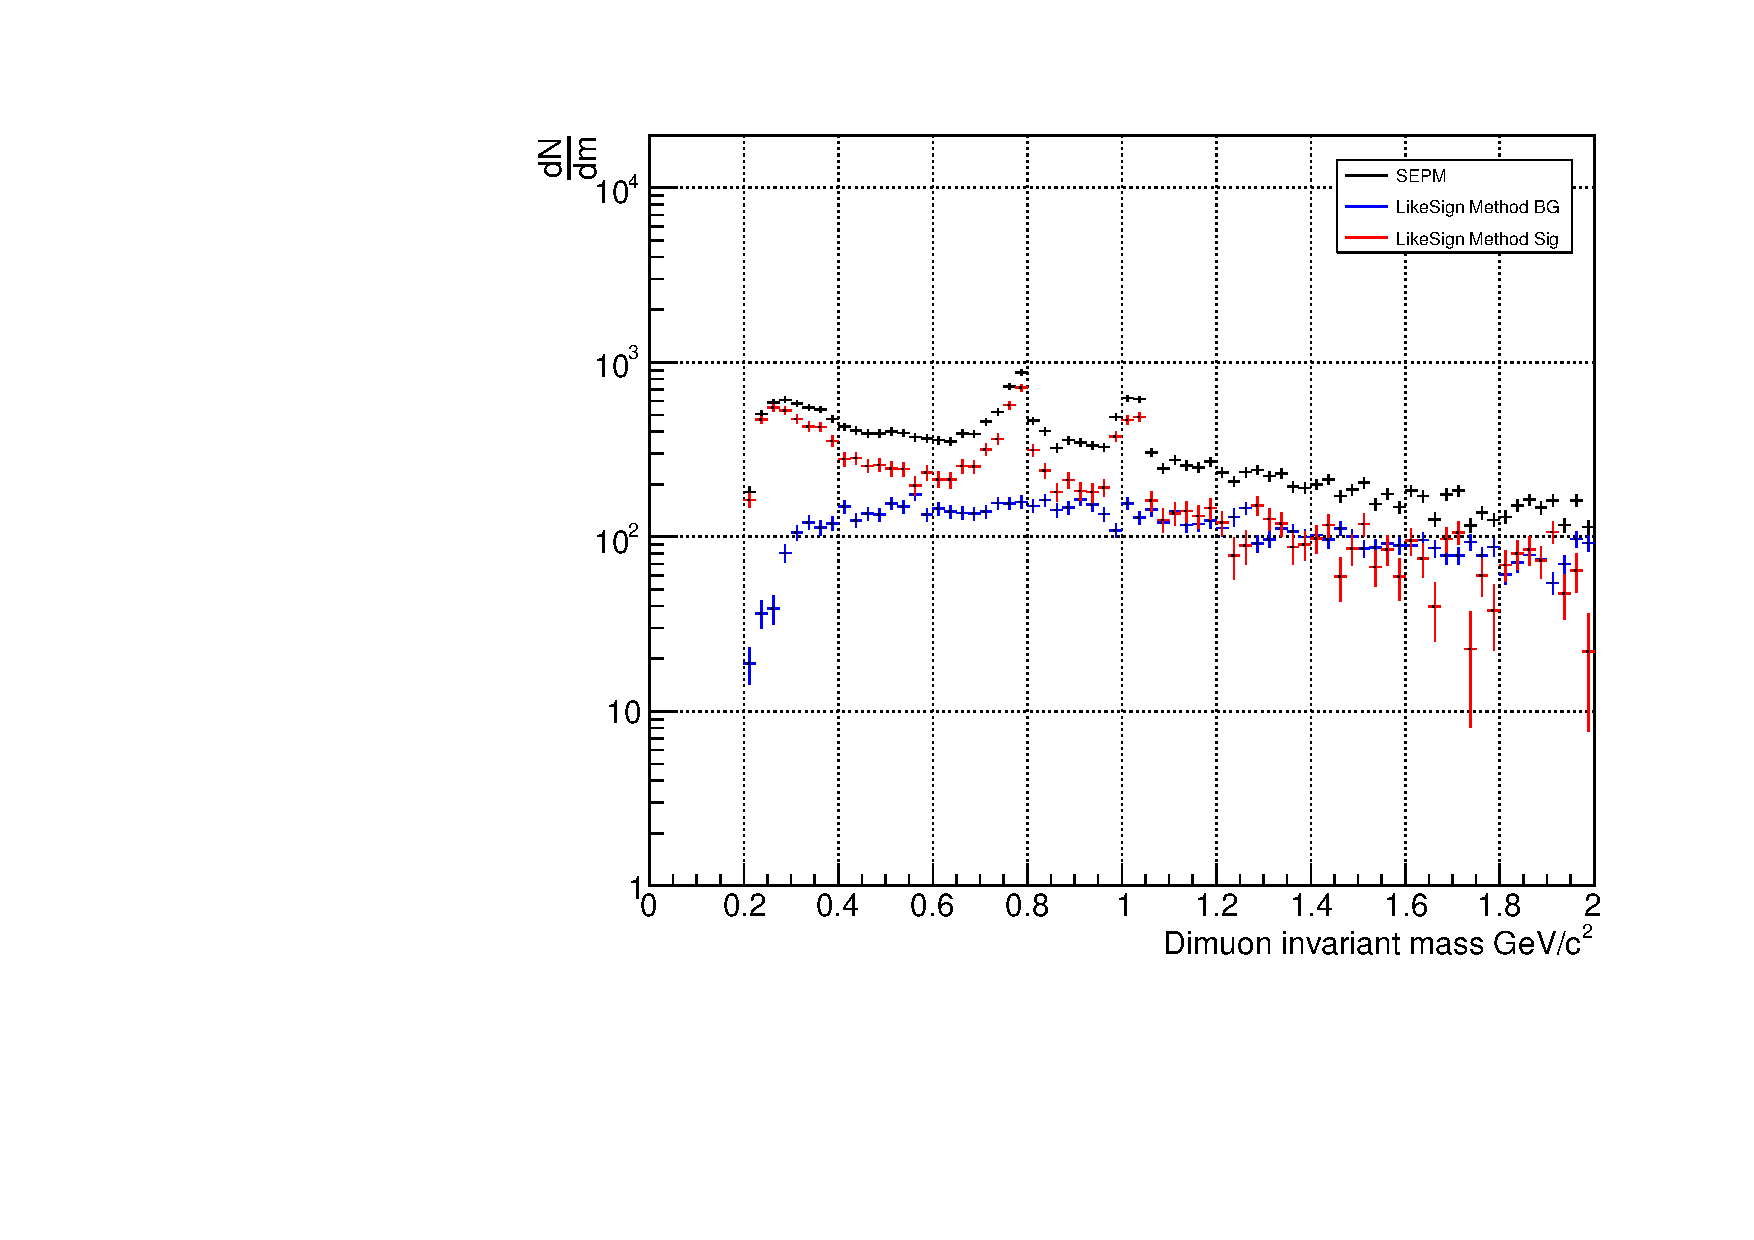
\includegraphics[width=\textwidth]{fig/3_4_1_CB_pt_3to4.pdf}
                        \caption*{3 < $p_{T}$ < 4}
                    \end{minipage}
                    \hfill
                    \begin{minipage}{0.45\textwidth}
                        \centering
                        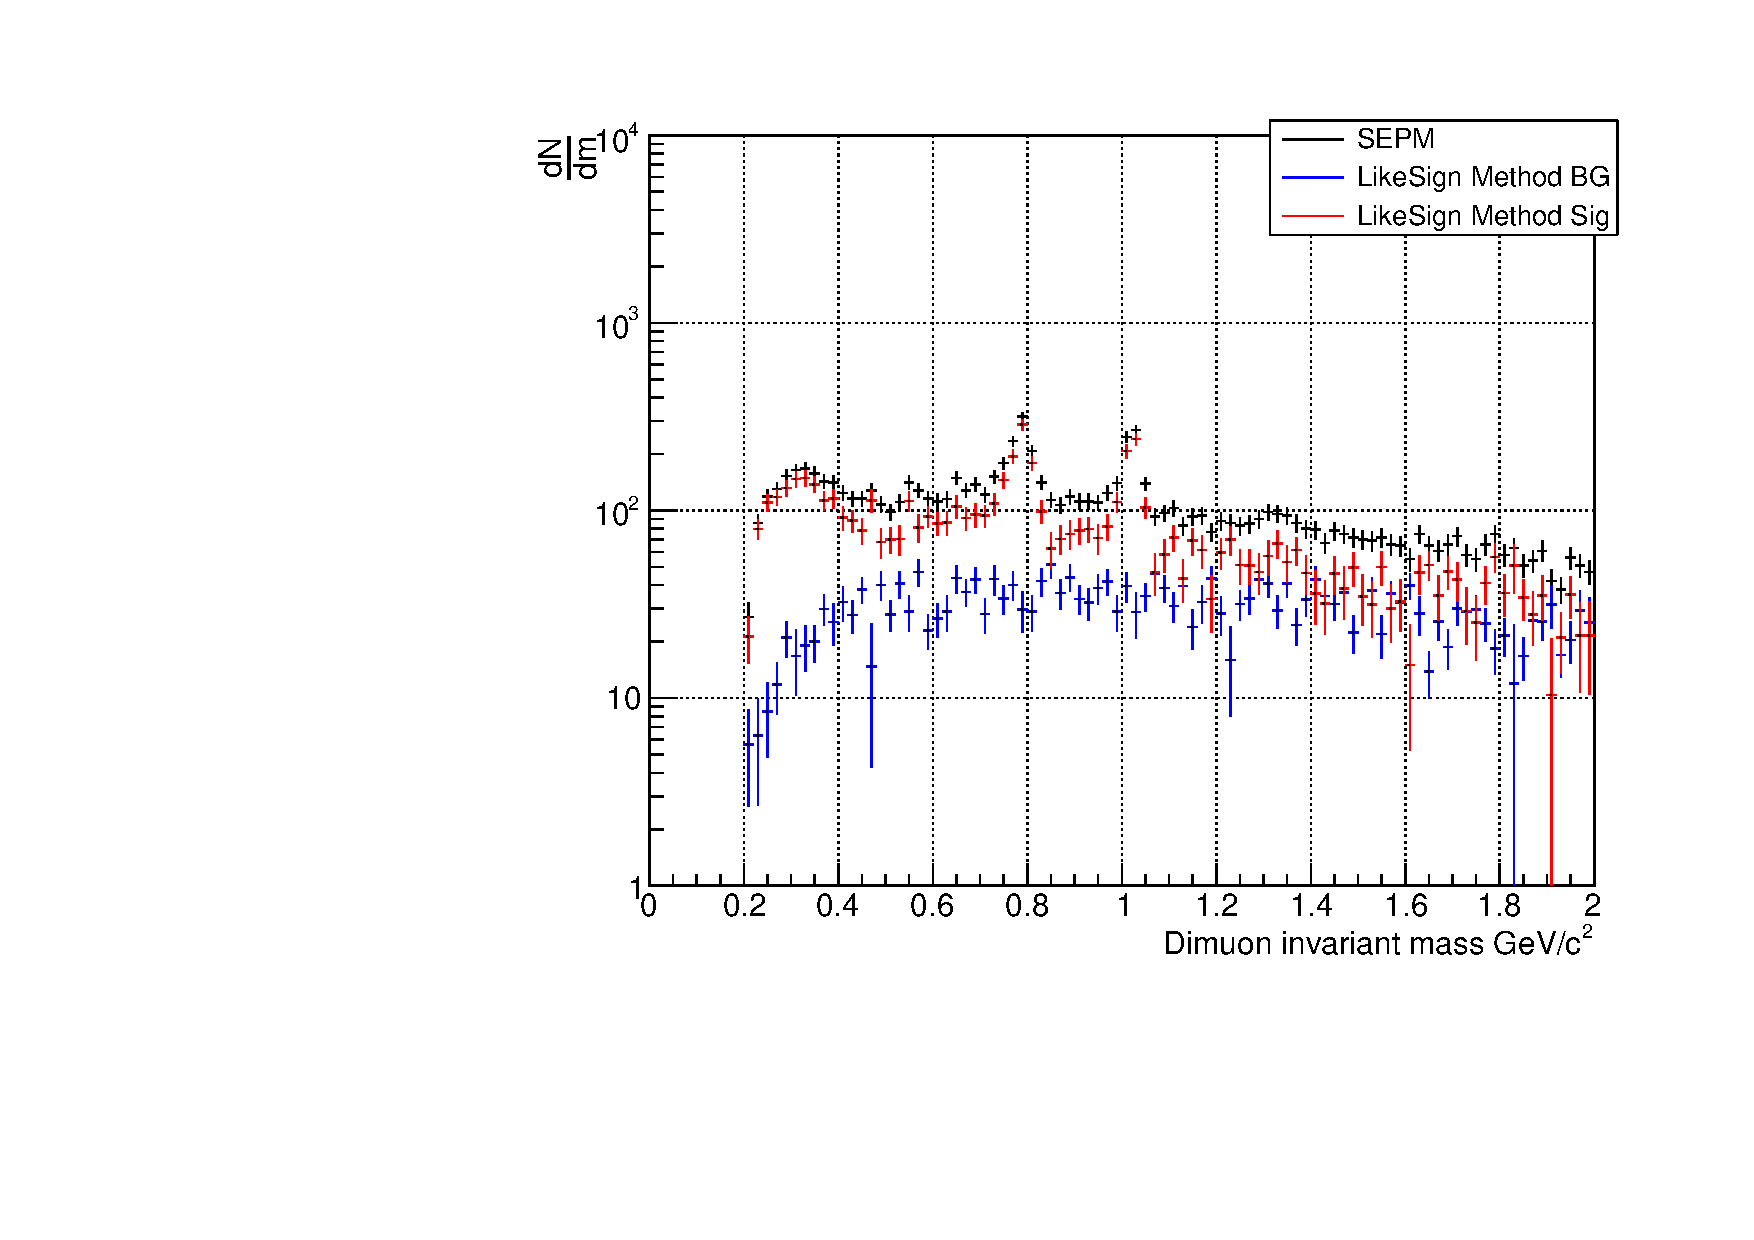
\includegraphics[width=\textwidth]{fig/3_4_1_CB_pt_4to5.pdf}
                        \caption*{4 < $p_{T}$ < 5}
                    \end{minipage}
                    \\
                    \vspace{1em}
                    \begin{minipage}{0.45\textwidth}
                        \centering
                        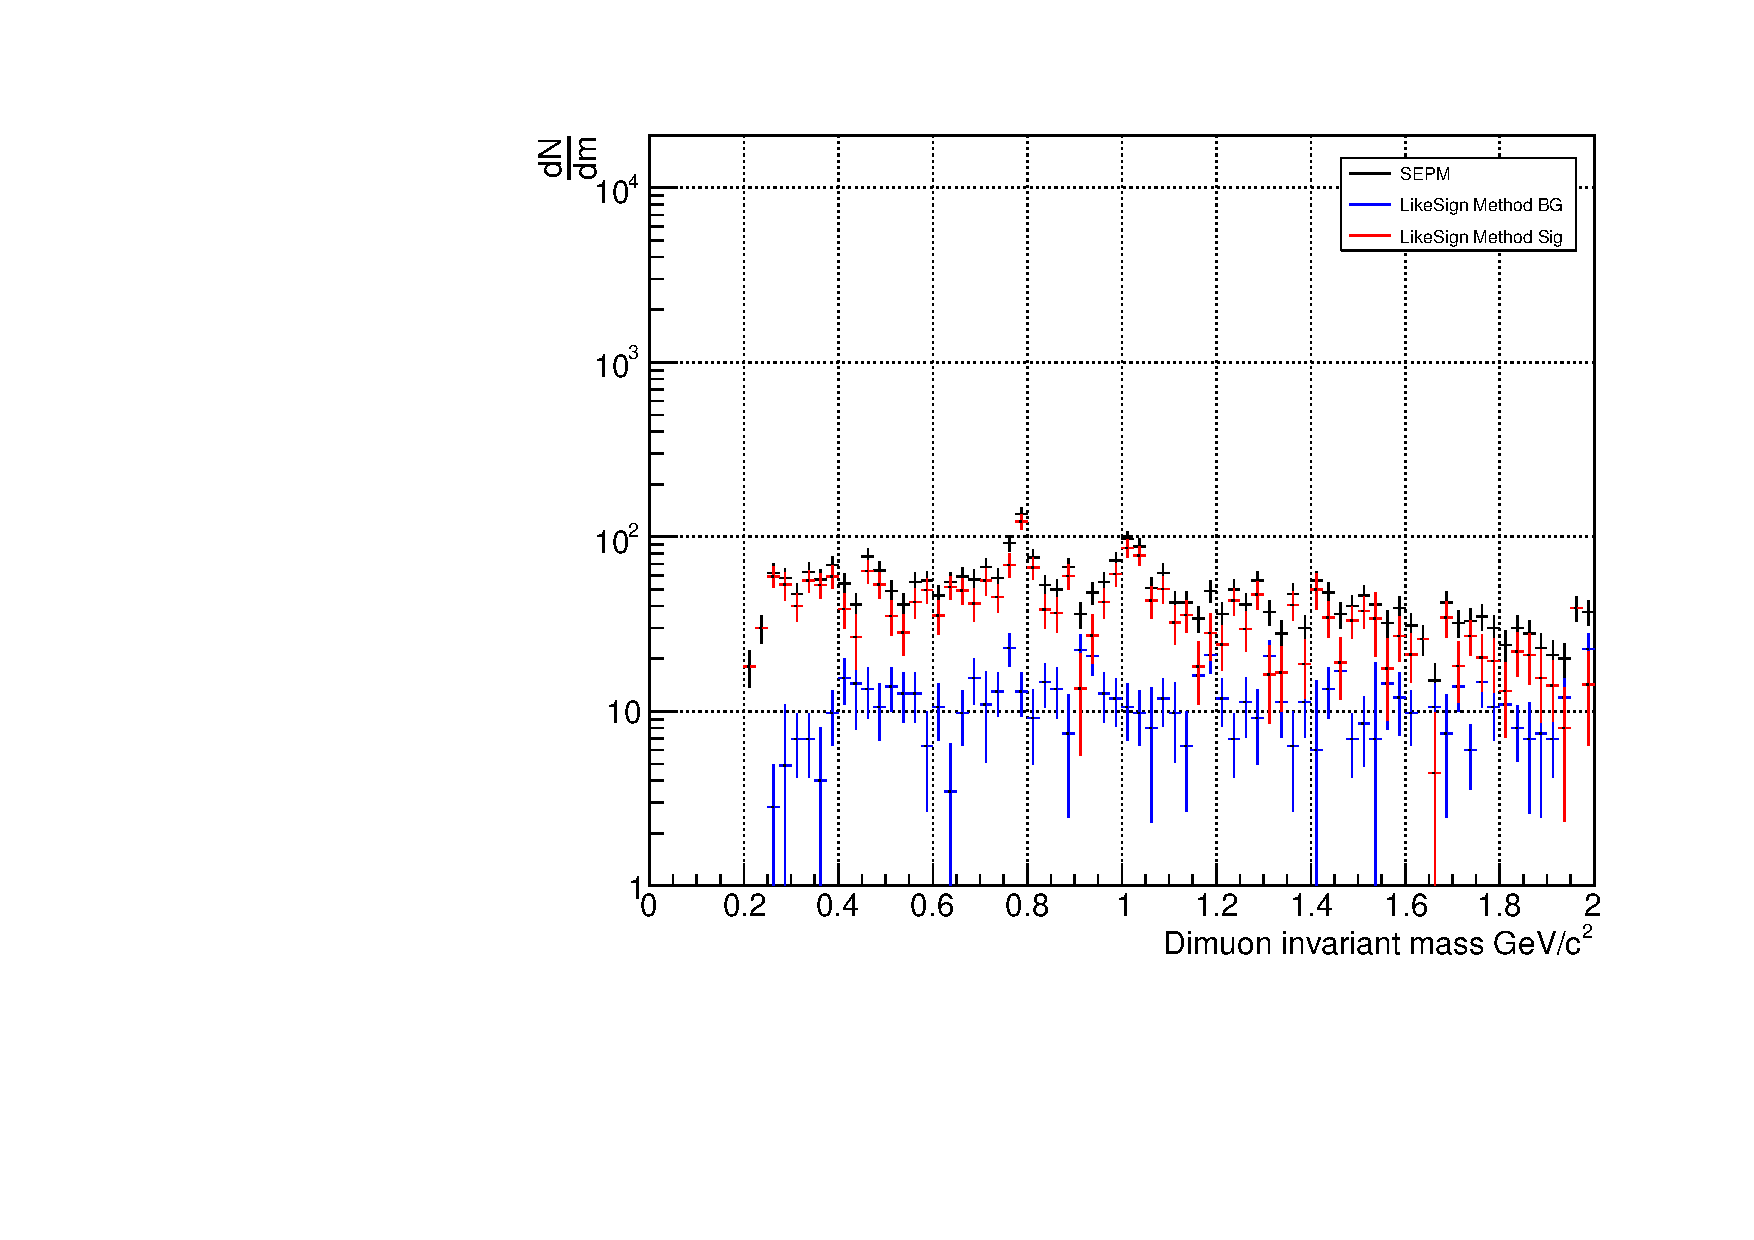
\includegraphics[width=\textwidth]{fig/3_4_1_CB_pt_5to6.pdf}
                        \caption*{5 < $p_{T}$ < 6}
                    \end{minipage}
                    \hfill
                    \begin{minipage}{0.45\textwidth}
                        \centering
                        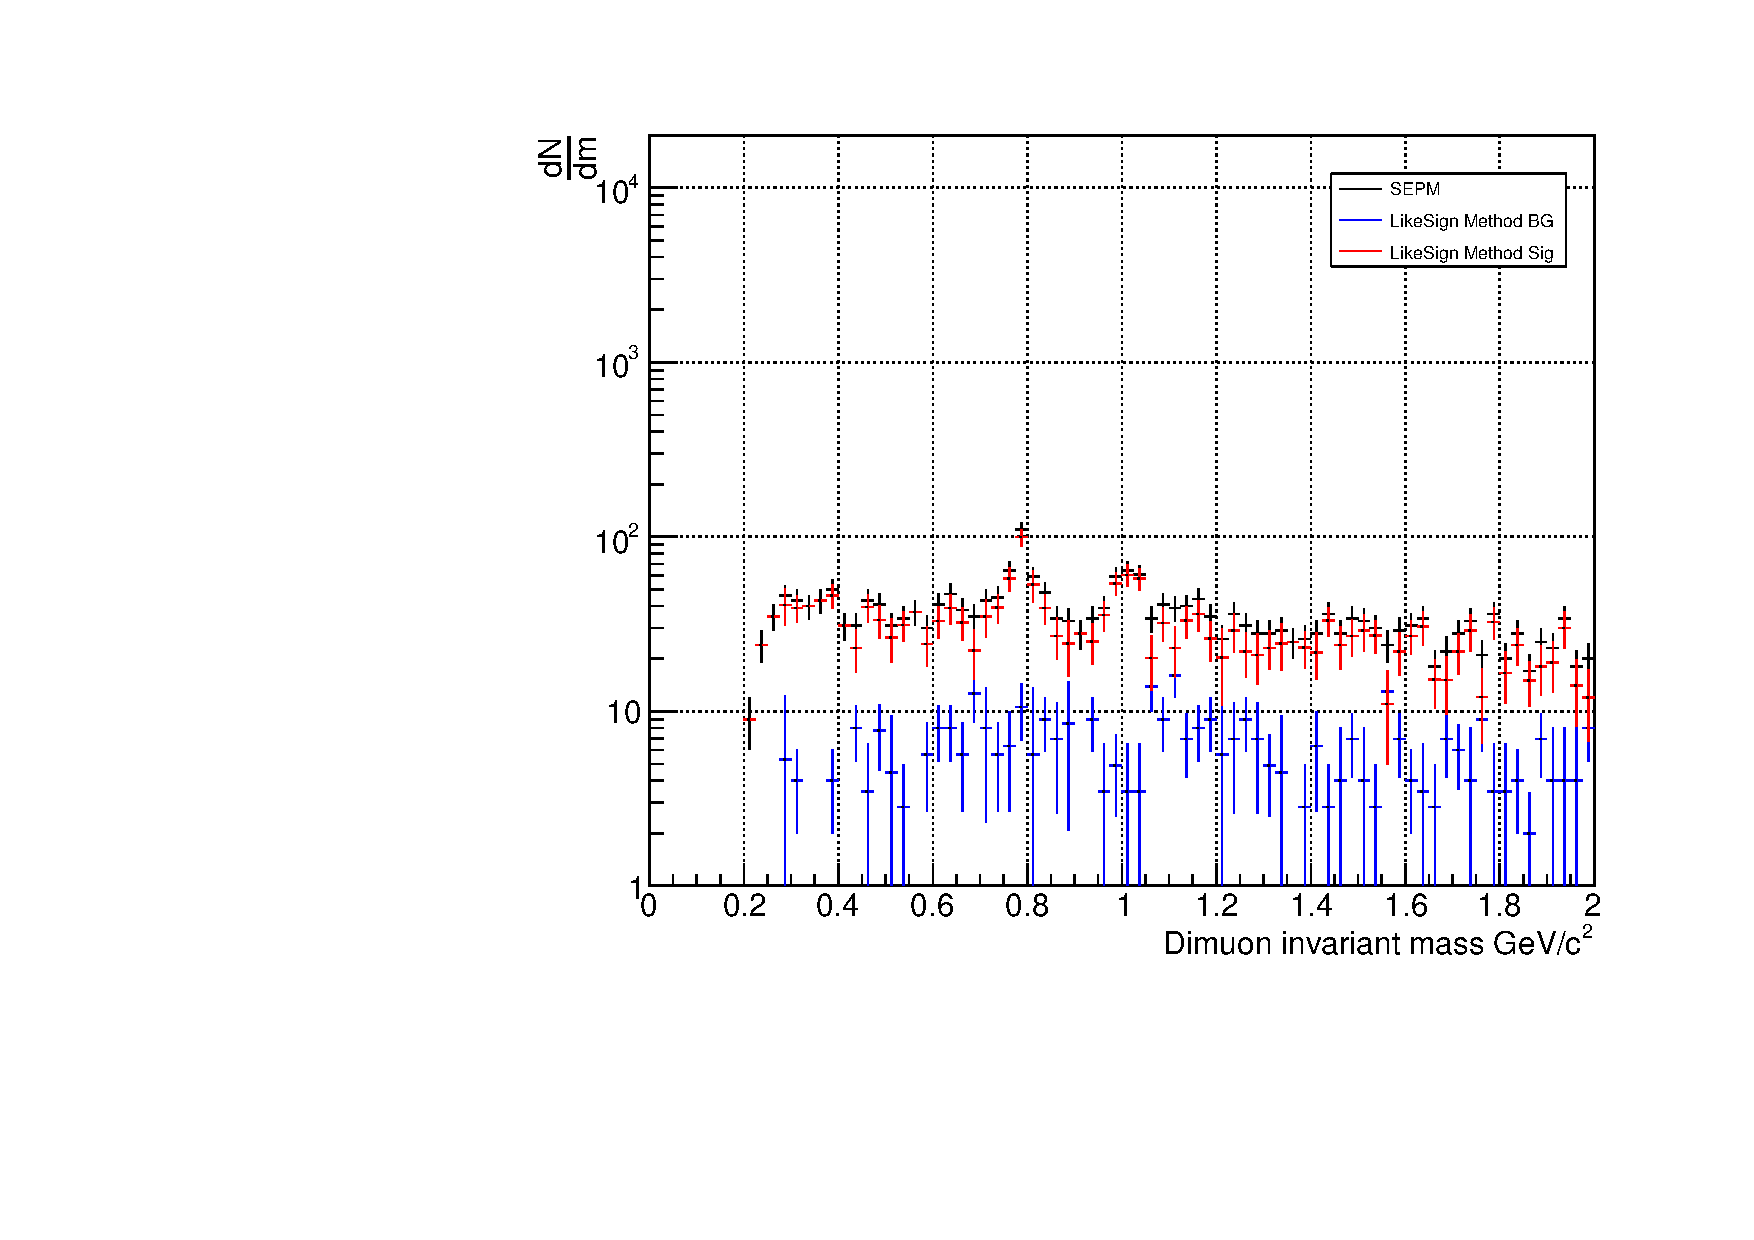
\includegraphics[width=\textwidth]{fig/3_4_1_CB_pt_6to10.pdf}
                        \caption*{6 < $p_{T}$ < 10}
                    \end{minipage}
                    \caption{Result of combinatorial background subtracktion of each $p_T$}
                    \label{Analysis:Dimuon:CB:CB_pt_separation}
                \end{figure}
                In the region of \(0 < p_T < 1\) GeV, no peaks for \(\omega\) and \(\phi\) were observed. The reason is believed to be the insufficient resolution of the single muon \(p_T\) and the dominance of tracks with incorrect MFT-MCH matching.
                The region of \(6 < p_T < 10\) GeV was chosen to be wider than other transverse momentum regions to preserve the statistical significance.
        
            \subsubsection{Peak extraction of $\omega \rightarrow \mu\mu ,\phi \rightarrow \mu\mu$}
            \label{Peak_extraction}
                The distributions of the correlated dimuon invariant mass obtained from \ref{Analysis:Dimuon:Combinatorial BG subtraction} are used to extract the distributions of $\omega \rightarrow \mu\mu,\phi \rightarrow \mu\mu$. The dimuon invariant mass distribution under 2($GeV/c^2$) contains pairs of muons coming from light and open heavy-flavor mesons. Charm and bottom quarks have heavy masses produced through pair creation in the initial collision. The pair-created \(c\bar{c}\) quarks separate and form \(D\bar{D}\) mesons. The \(D\) and \(\bar{D}\) mesons undergo semileptonic decays, such as \(D \rightarrow \bar{K}^0 + \mu^+ + \nu_\mu\) or \(D \rightarrow \mu^+ + \nu_\mu\), and \(\bar{D} \rightarrow K^0 + \mu^- + \nu_\mu\) or \(\bar{D} \rightarrow \mu^- + \nu_\mu\). Since the parent \(D\) and \(\bar{D}\) mesons are produced through pair creation, they are strongly correlated, and their decay products, the muons, also exhibit correlation. As a result, the dimuon mass distribution with correlations is included. The same correlation applies in the case of \(B\) mesons.
                \begin{itemize}
                    \item $\eta \rightarrow \mu^+ \mu^-$
                    \item $\eta \rightarrow \mu^+ \mu^- \gamma$
                    \item $\rho \rightarrow \mu^+ \mu^-$
                    \item $\omega \rightarrow \mu^+ \mu^-$
                    \item $\omega \rightarrow \mu^+ \mu^- \pi^0$
                    \item $\eta' \rightarrow \mu^+ \mu^- \gamma$
                    \item $\phi \rightarrow \mu^+ \mu^-$
                    \item $c\bar{c} \rightarrow D\bar{D} \rightarrow \mu^+ \mu^- + others$
                    \item $b\bar{b} \rightarrow B\bar{B} \rightarrow \mu^+ \mu^- + others$
                \end{itemize}
                The decays \(\omega \rightarrow \mu\mu\) and \(\phi \rightarrow \mu\mu\) are known to exhibit sharp peak structures from previous lepton pair measurements, forming peaks near 0.8 \(\mathrm{GeV/c^2}\) and 1.0 \(\mathrm{GeV/c^2}\) in the mass distribution.
                It is known that no sharp peak structures exist for any decays other than the two-body decays of \(\omega\) and \(\phi\). Therefore, the continuous component was fitted using an exponential function. The fitting was performed in the range of 0.5 < \(M_{\mu\mu}\) < 1.3 \(\mathrm{GeV/c^2}\), excluding the regions with peak structures at 0.7 < \(M_{\mu\mu}\) < 0.86 and 0.92 < \(M_{\mu\mu}\) < 1.15. The continuous component was fitted using the exponential function shown (\ref{fit:BG}).
                \begin{eqnarray}
                    \label{fit:BG}
                    f_{BG}(m)=N_0*\exp{-p1* m}
                \end{eqnarray}
                where, \(N_0\) and \(p1\) are the fit parameters. The continuous component mass distribution was subtracted using the results from the fit. Gaussian fits were performed for the \(\omega\) and \(\phi\) in the mass regions 0.7 < \(M_{\mu\mu}\) < 0.86 \(\mathrm{GeV/c^2}\) and 0.92 < \(M_{\mu\mu}\) < 1.15 \(\mathrm{GeV/c^2}\), respectively. The fitting function is given by (\ref{fit:omega}) and (\ref{fit:phi}).
                \begin{eqnarray}
                    \label{fit:omega}
                    f_{\omega} &=& N_{\omega}*\exp{-\frac{1}{2}\qty(\frac{m-M_{\omega}}{\sigma_{\omega}})^2}\\\
                    \label{fit:phi}
                    f_{\phi} &=& N_{\phi}*\exp{-\frac{1}{2}\qty(\frac{m-M_{\phi}}{\sigma_{\phi}})^2}
                \end{eqnarray}
                The fit parameters are \(N_{\omega}, N_{\phi}, M_{\omega}, M_{\phi}, \sigma_{\omega}, \sigma_{\phi}\). Specifically, \(M_{\omega}\) and \(M_{\phi}\) correspond to the mean mass positions of \(\omega\) and \(\phi\), while \(\sigma_{\omega}\) and \(\sigma_{\phi}\) correspond to the mass widths. Using the fit parameters obtained from the continuous component and the Gaussian fits for \(\omega\) and \(\phi\), all functions were combined, and a global fit was performed to extract the mean mass positions and mass widths of \(\omega\) and \(\phi\). The fit range is 0.5 < \(M_{\mu\mu}\) < 1.3 \(\mathrm{GeV/c^2}\). The function for the overall fit is given by the (\ref{fit:globalfit}).
                \begin{eqnarray}
                    \label{fit:globalfit}
                    f(m)=N_0*\exp{-p1* m}+N_{\omega}*\exp{-\frac{1}{2}\qty(\frac{m-M_{\omega}}{\sigma_{\omega}})^2}+N_{\phi}*\exp{-\frac{1}{2}\qty(\frac{m-M_{\phi}}{\sigma_{\phi}})^2}
                \end{eqnarray}
                The parameters for the overall fit are similarly \(N_0, N_{\omega}, N_{\phi}, M_{\omega}, M_{\phi}, \sigma_{\omega}, \sigma_{\phi}\). The fit results are shown in Figure \ref{Analysis:Dimuon:Yield:fit} and Table \ref{Analysis:Dimuon:Yield:Fit_Results}.
                \begin{figure}[H]
                    \centering
                    \begin{minipage}{0.45\textwidth}
                        \centering
                        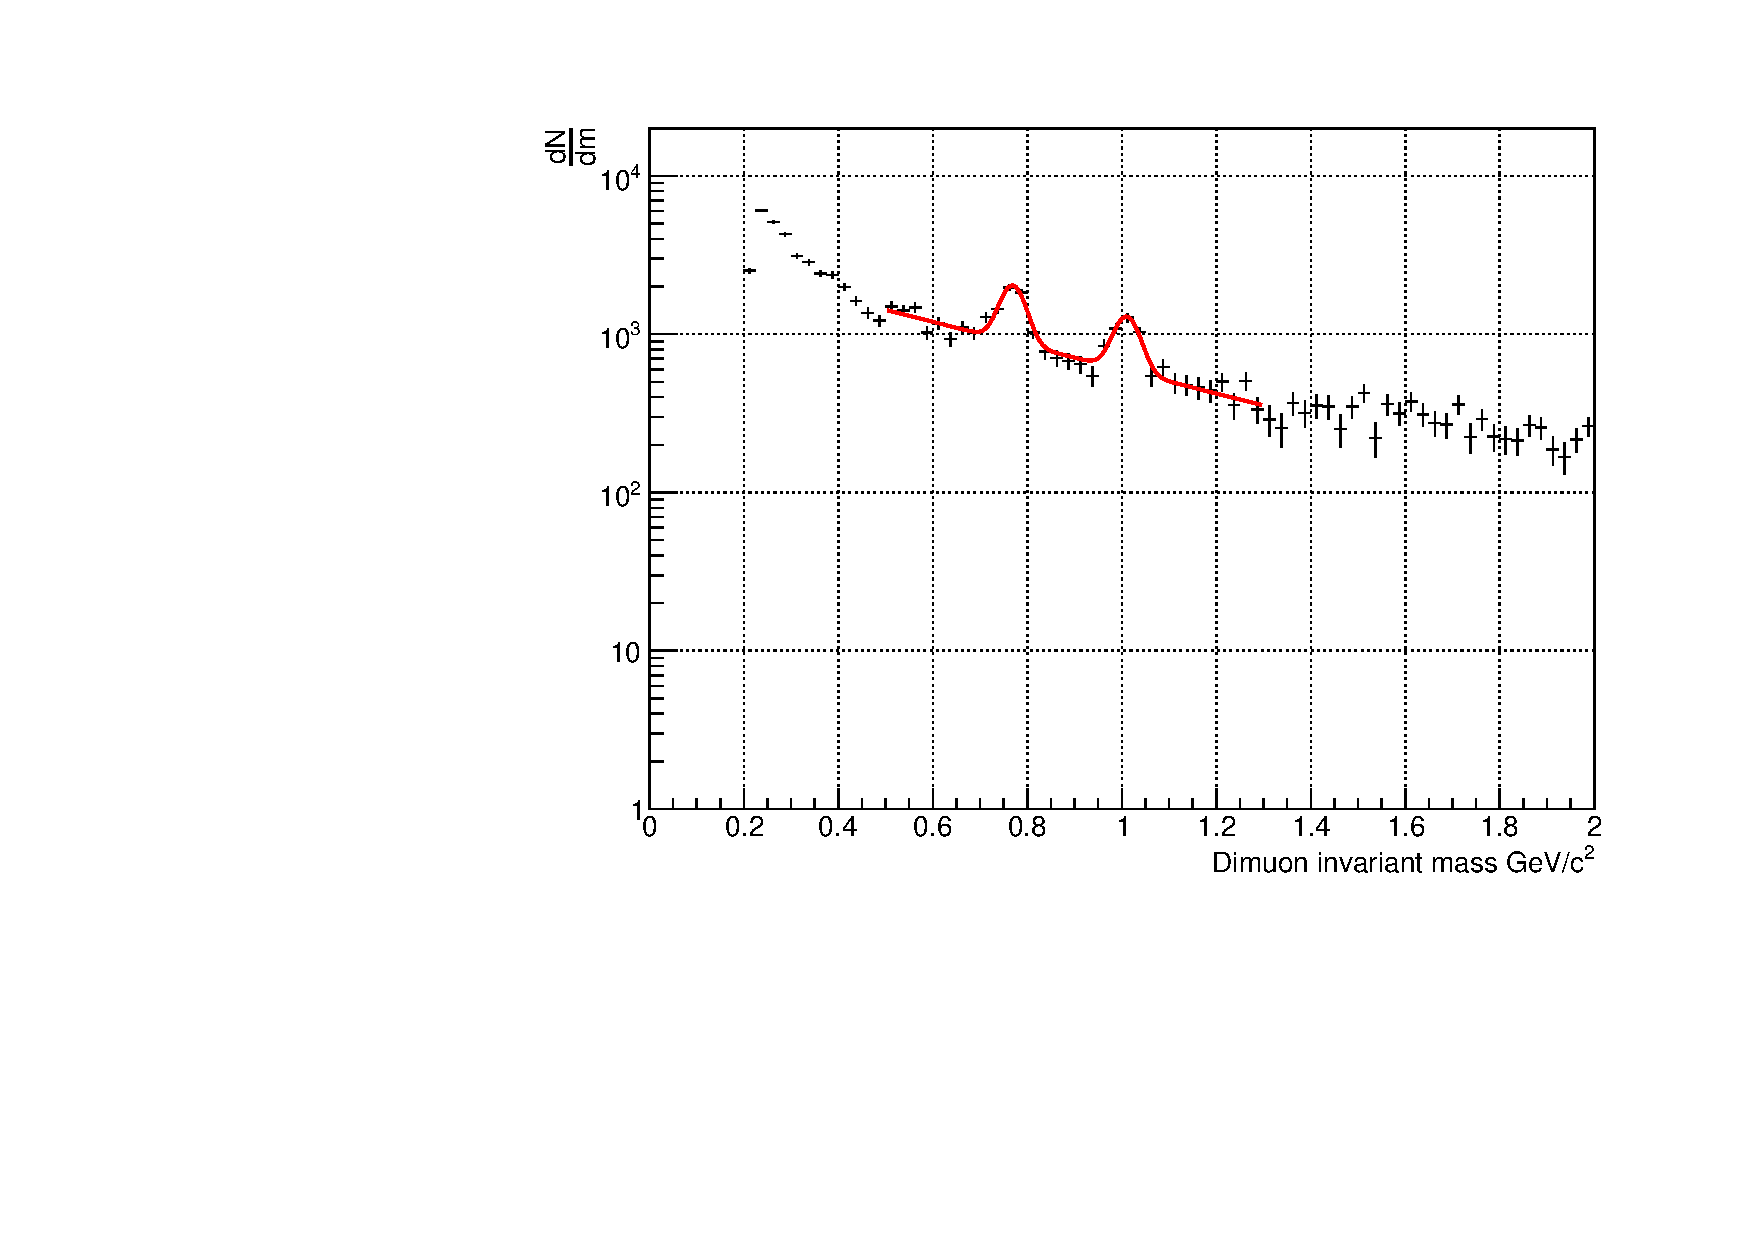
\includegraphics[width=\textwidth]{fig/3_4_2_fit_pt_1to2.pdf}
                        \captionsetup{labelformat=empty}
                        \caption*{1 < $p_{T}$ < 2}
                    \end{minipage}
                    \hfill
                    \begin{minipage}{0.45\textwidth}
                        \centering
                        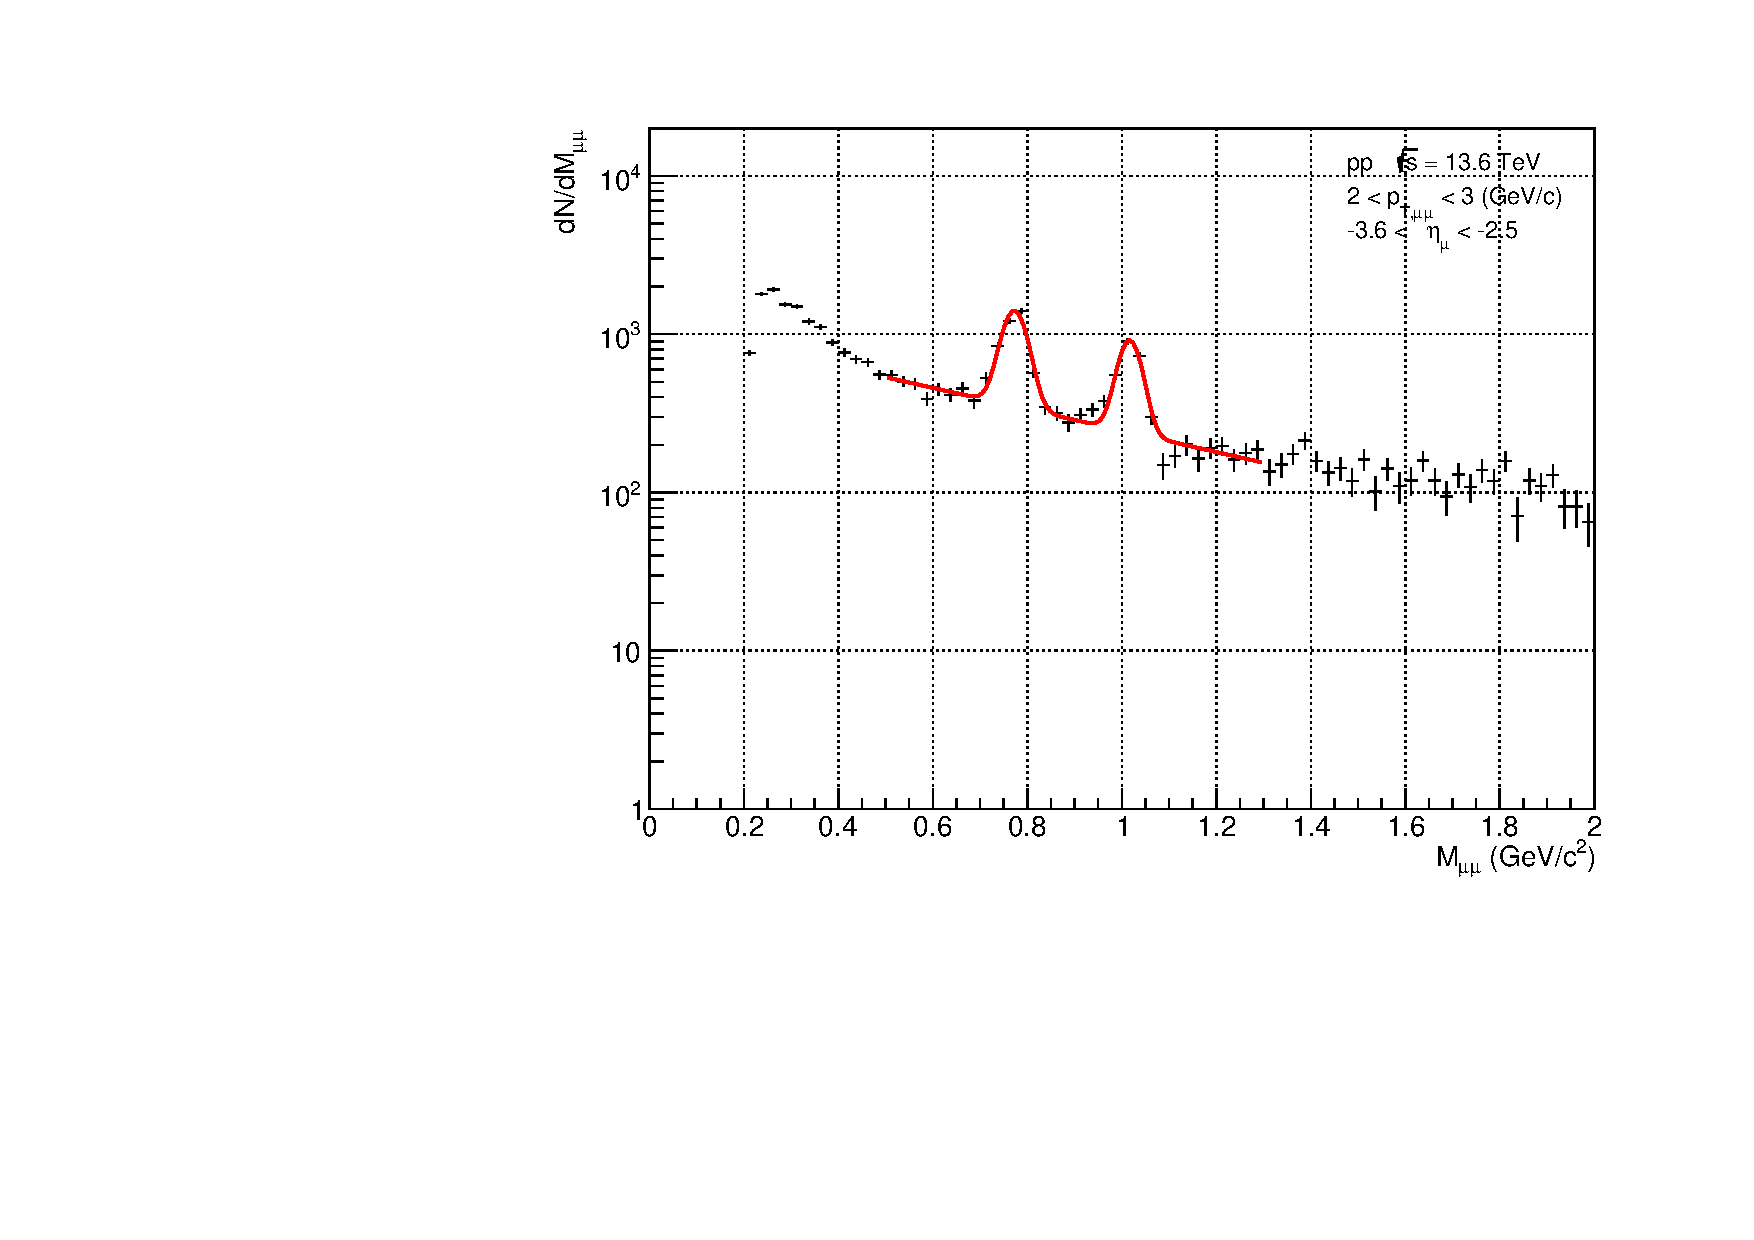
\includegraphics[width=\textwidth]{fig/3_4_2_fit_pt_2to3.pdf}
                        \captionsetup{labelformat=empty}
                        \caption*{2 < $p_{T}$ < 3}
                    \end{minipage}
                    \\
                    \vspace{1em}
                    \begin{minipage}{0.45\textwidth}
                        \centering
                        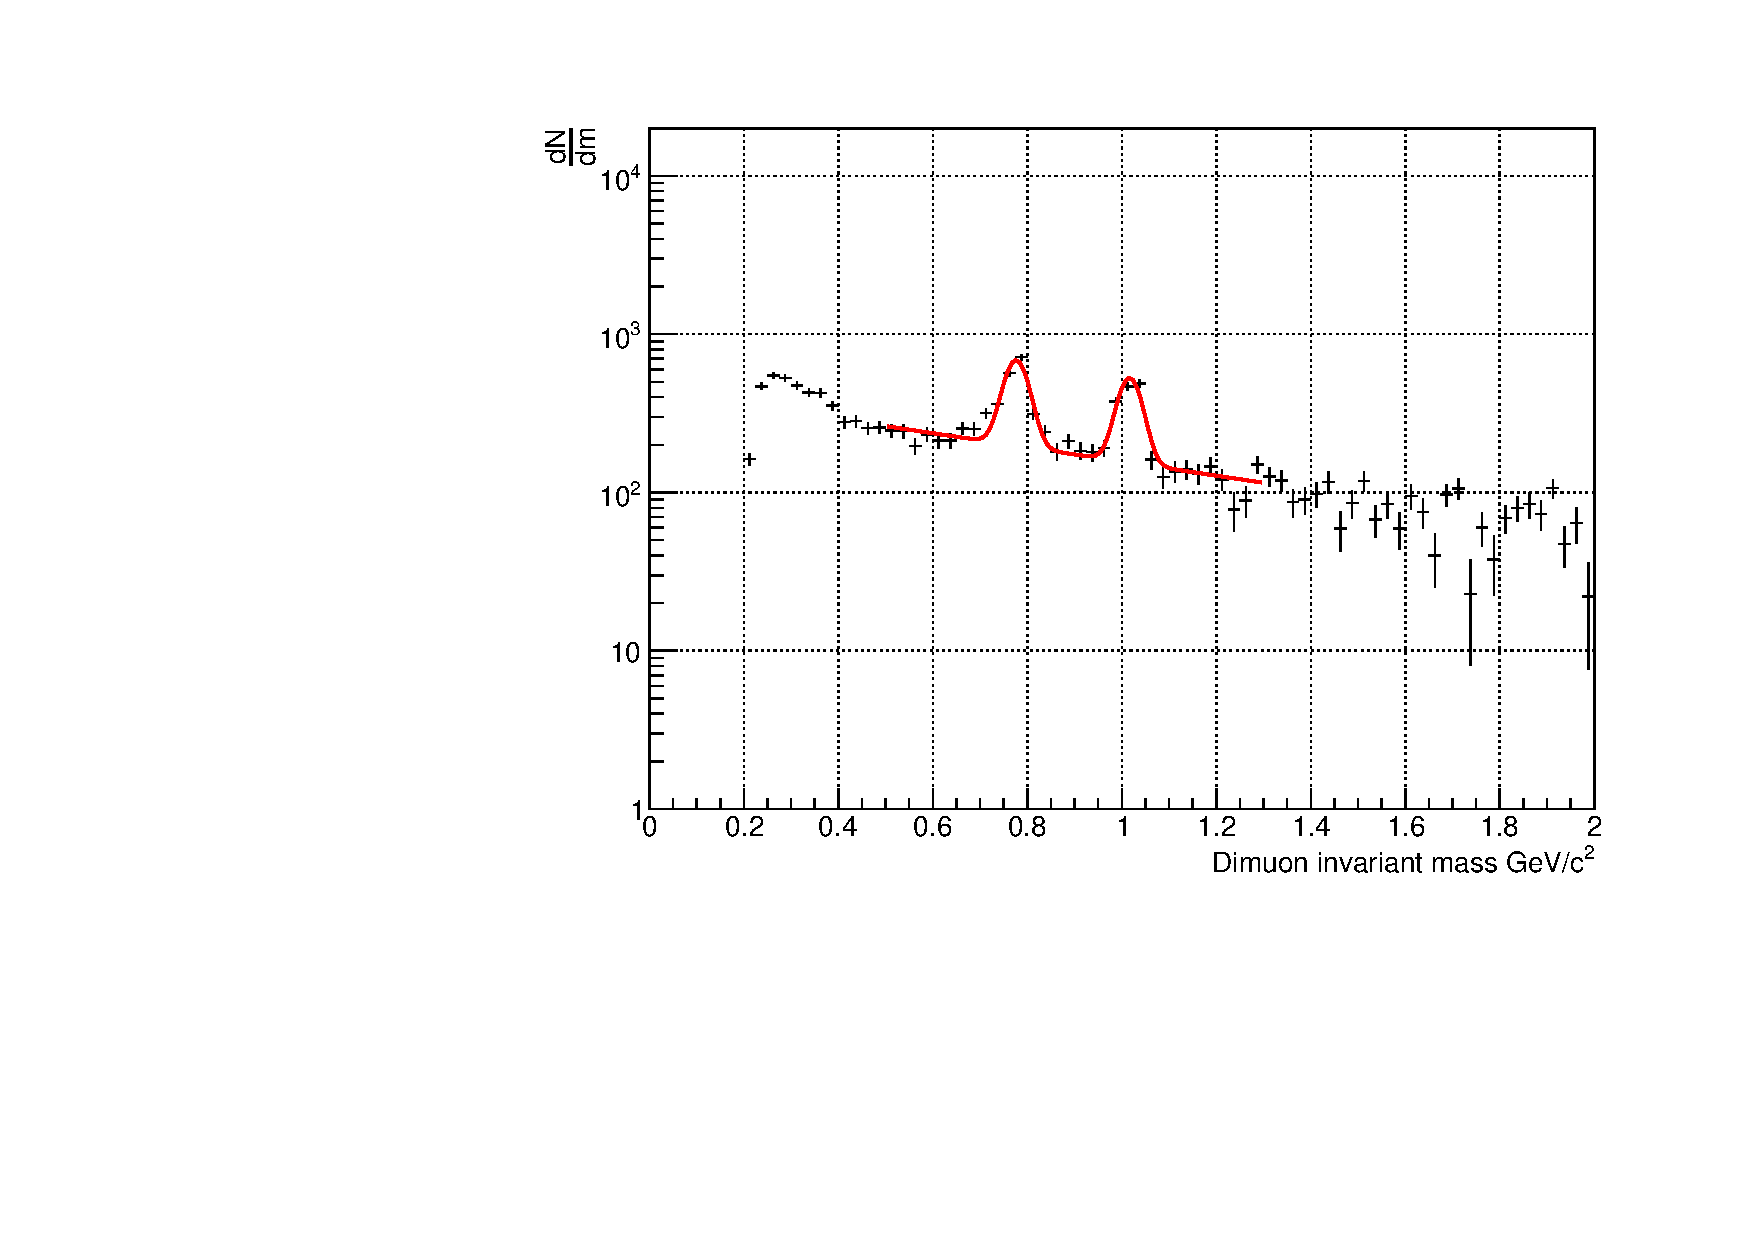
\includegraphics[width=\textwidth]{fig/3_4_2_fit_pt_3to4.pdf}
                        \captionsetup{labelformat=empty}
                        \caption*{3 < $p_{T}$ < 4}
                    \end{minipage}
                    \hfill
                    \begin{minipage}{0.45\textwidth}
                        \centering
                        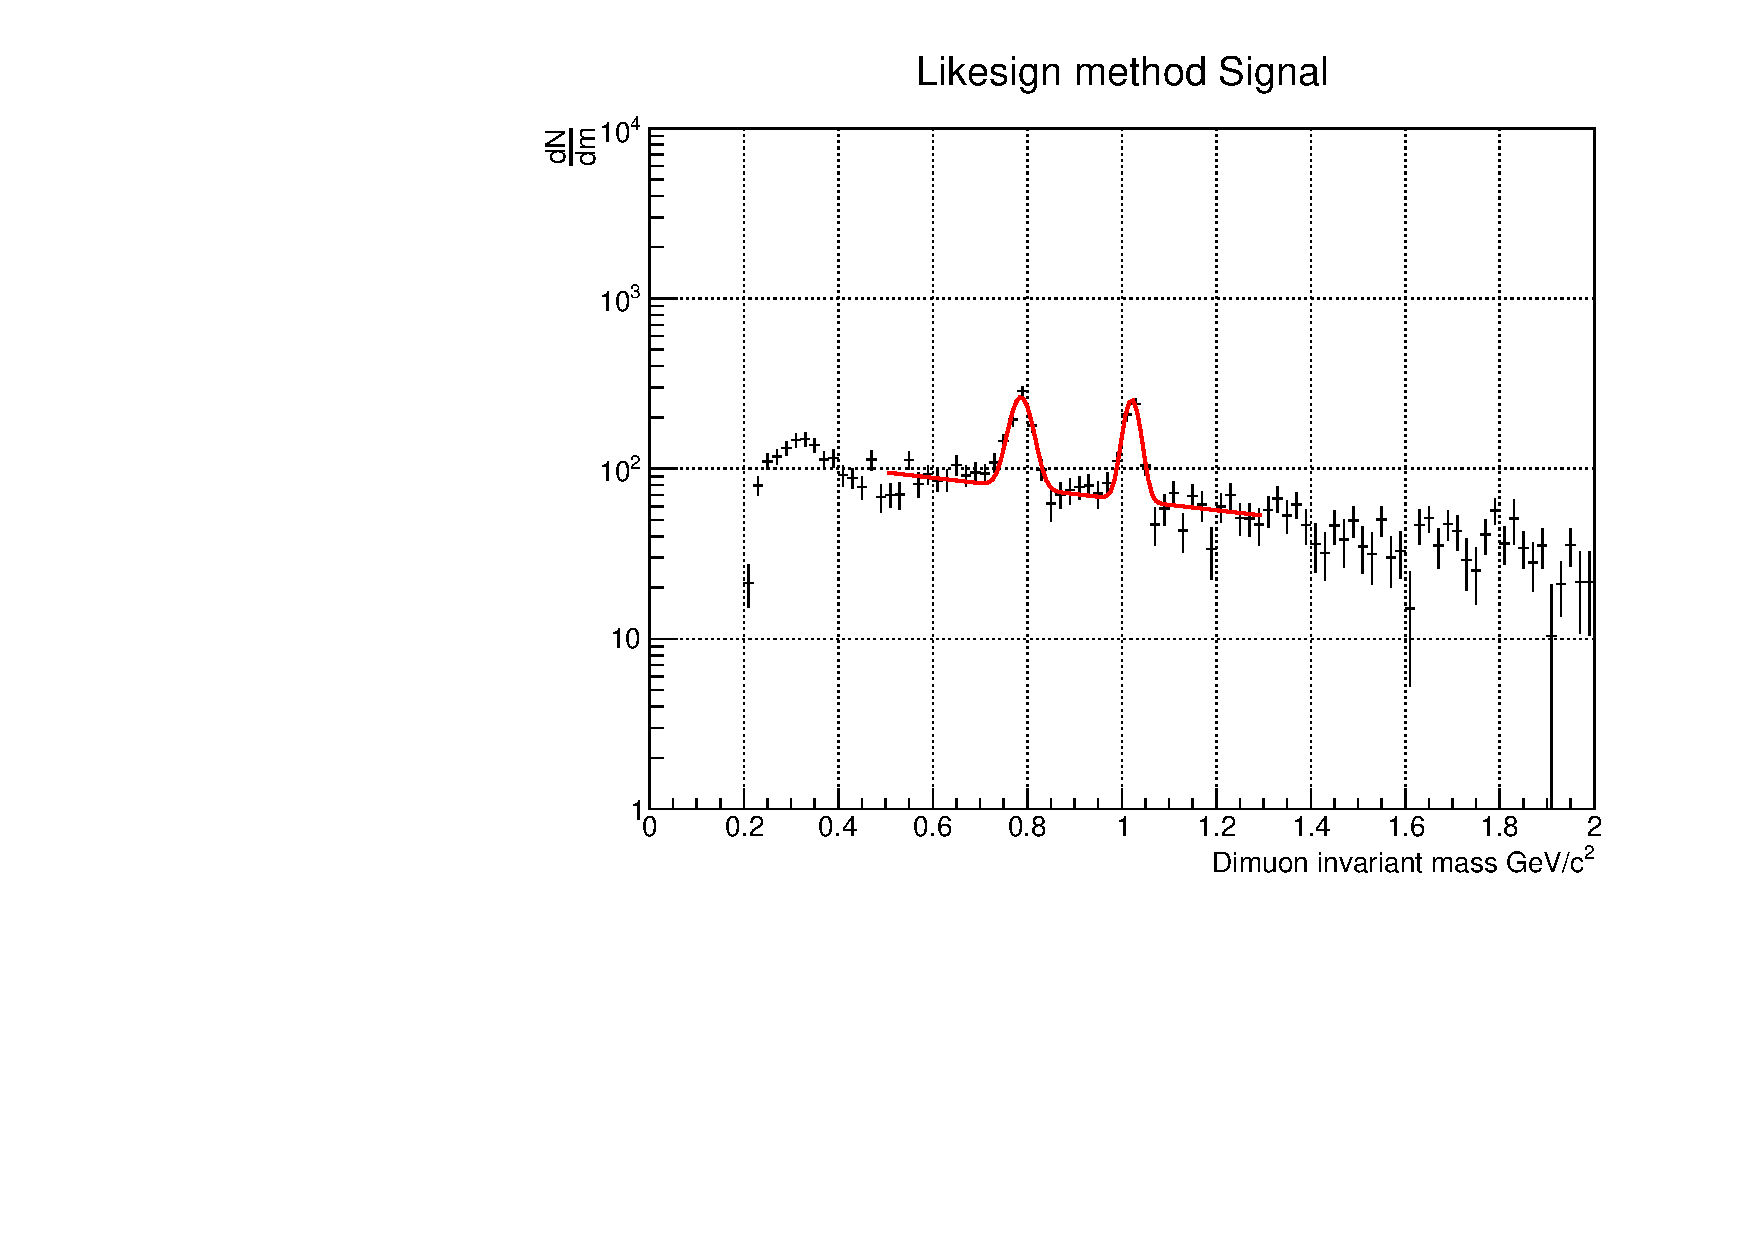
\includegraphics[width=\textwidth]{fig/3_4_2_fit_pt_4to5.pdf}
                        \captionsetup{labelformat=empty}
                        \caption*{4 < $p_{T}$ < 5} 
    
                    \end{minipage}
                    \\
                    \vspace{1em}
                    \begin{minipage}{0.45\textwidth}
                        \centering
                        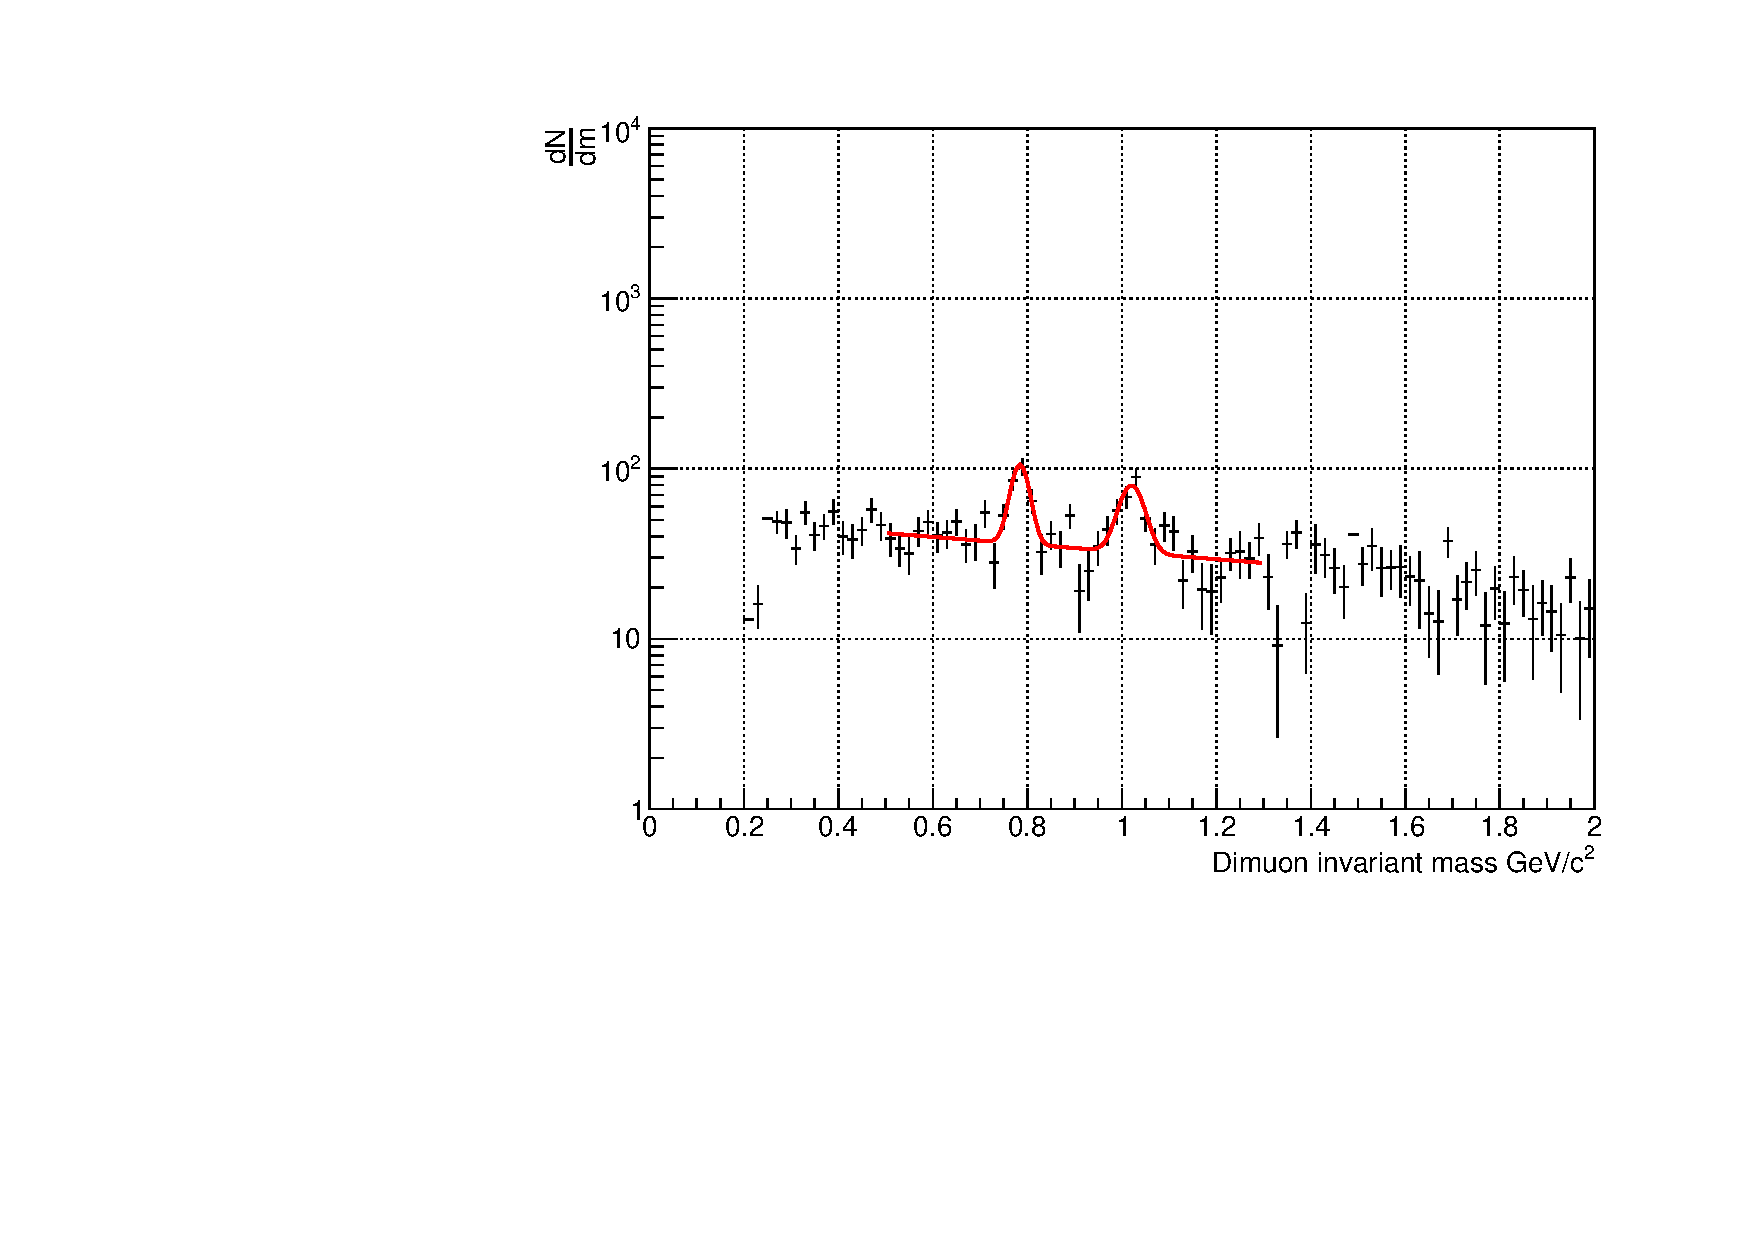
\includegraphics[width=\textwidth]{fig/3_4_2_fit_pt_5to6.pdf}
                        \captionsetup{labelformat=empty}
                        \caption*{5 < $p_{T}$ < 6}
                    \end{minipage}
                    \hfill
                    \begin{minipage}{0.45\textwidth}
                        \centering
                        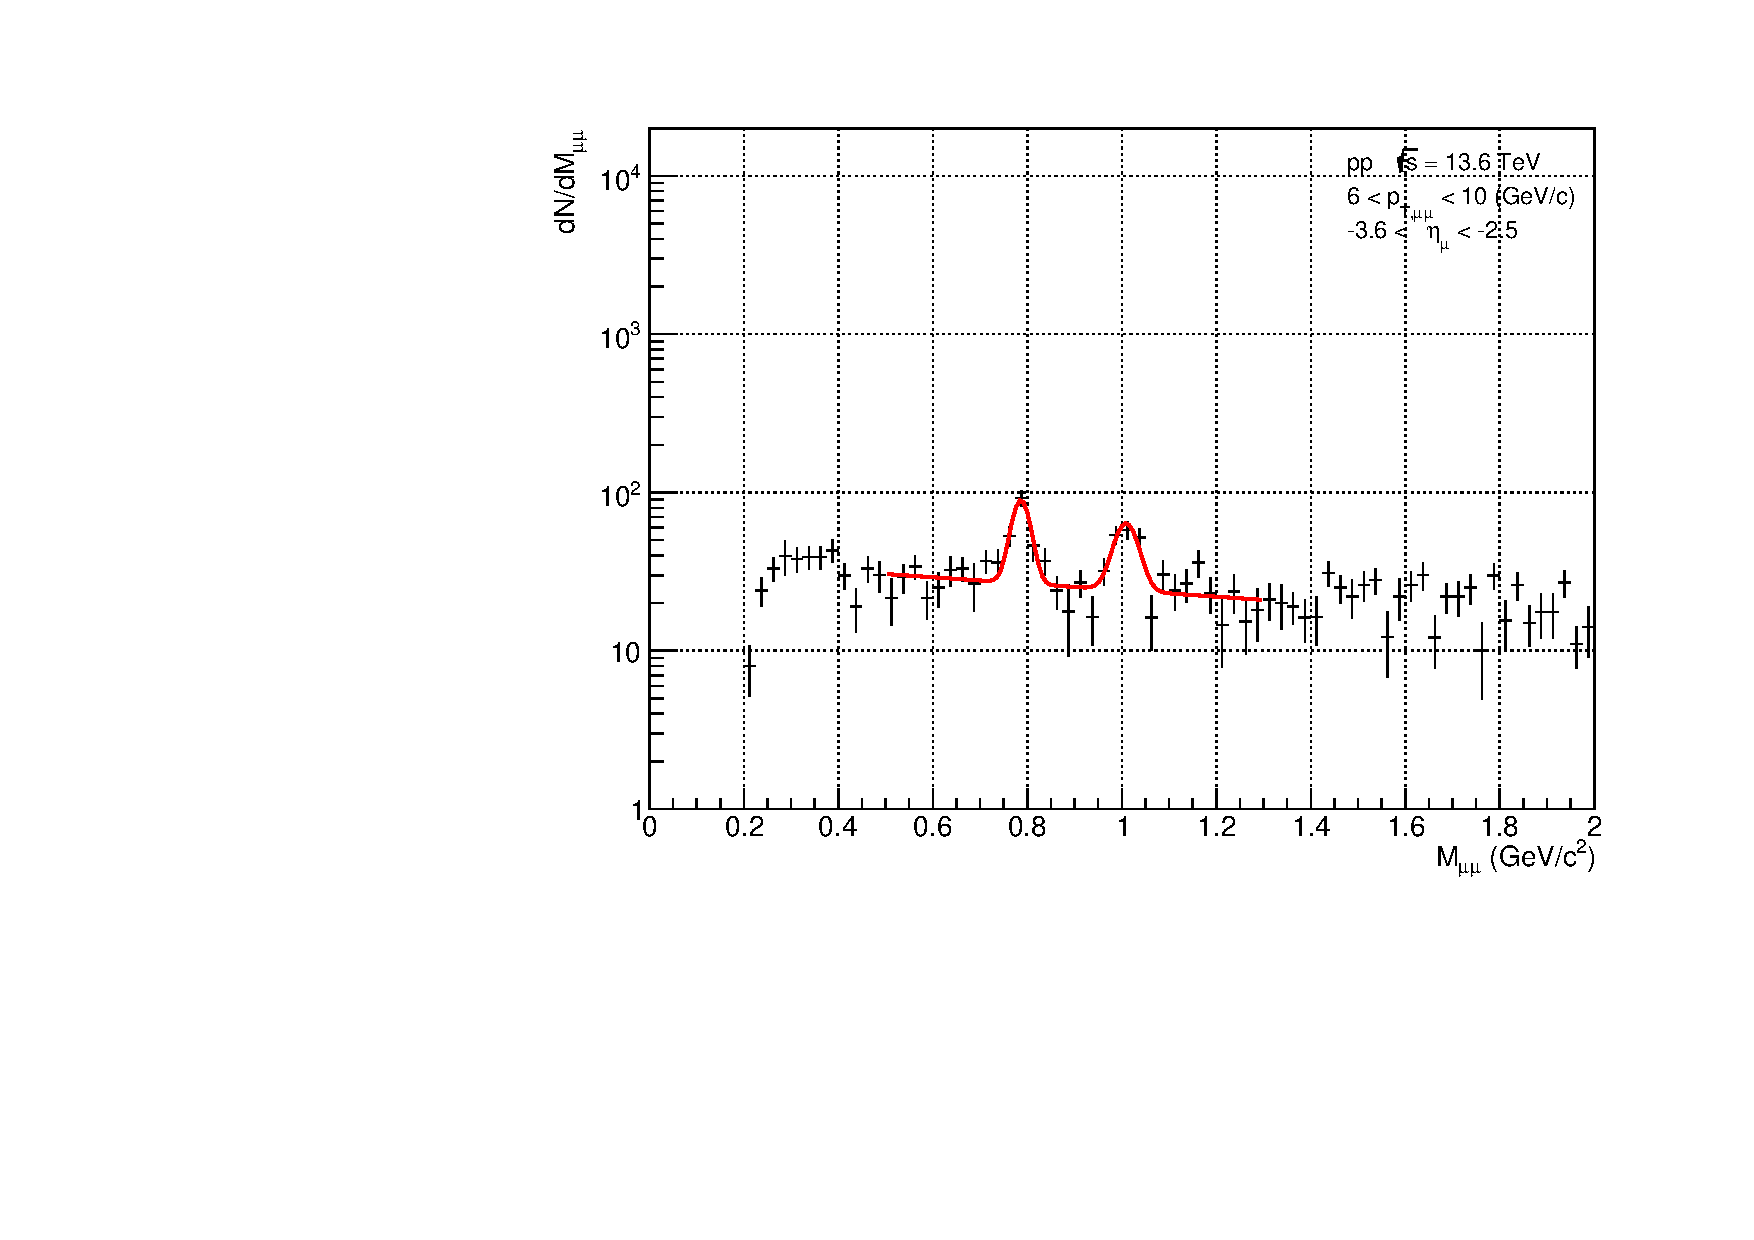
\includegraphics[width=\textwidth]{fig/3_4_2_fit_pt_6to10.pdf}
                        \captionsetup{labelformat=empty}
                        \caption*{6 < $p_{T}$ < 10}
                    \end{minipage}
                    \caption{fit result of each pt}
                    \label{Analysis:Dimuon:Yield:fit}
                \end{figure}
                The mean mass positions and mass widths of \(\omega\) and \(\phi\) for each transverse momentum, as well as the \(\chi^2\) of the fit, are summarised in the following table.
                    \begin{table}[htbp]
                        \centering
                        \caption{Fit Results}
                        \resizebox{\textwidth}{!}{
                            \begin{tabular}{|c||c|c|c|c|c|}
                                \hline
                                & $\omega$ mean mass & $\omega$ mass width & $\phi$ mean mass & $\phi$ mass width & fit $\chi^2$ \\ \hline \hline
                                1 < $p_{T}$ < 2 &$0.769\pm0.002$& $0.025\pm0.002$ &$1.010\pm0.002$ &$0.026\pm 0.002$ & 47.74/24\\ \hline
                                2 < $p_{T}$ < 3 &$0.773\pm0.001$&$0.026\pm0.001$ & $1.017\pm0.001$& $0.024\pm 0.001$ & 58.80/24\\ \hline
                                3 < $p_{T}$ < 4 &$0.775\pm0.002$& $0.026\pm0.002$ &$1.016\pm0.002$ &$0.025\pm 0.002$ & 76.50/24\\ \hline
                                4 < $p_{T}$ < 5 &$0.785\pm0.002$& $0.024\pm0.002$ &$1.018\pm0.002$ &$0.021\pm 0.002$ & 53.96/24\\ \hline
                                5 < $p_{T}$ < 6 &$0.789\pm0.003$& $0.018\pm0.003$ &$1.016\pm0.005$ &$0.026\pm 0.005$ & 36.85/24\\ \hline
                                6 < $p_{T}$ < 10 &$0.786\pm0.003$& $0.019\pm0.004$ &$1.009\pm0.005$ &$0.024\pm 0.003$ & 27.12/24\\ \hline
                            \end{tabular}
                        }
                        \label{Analysis:Dimuon:Yield:Fit_Results}
                    \end{table}
        \subsubsection{Yield calculation of $\omega,\phi$} 
            The yield for each meson was calculated using the mean mass position and mass width of $\omega \rightarrow \mu\mu$ and $\phi \rightarrow \mu\mu$ obtained from the above fit. The number of dimuons falling within 3$\sigma$ of each Gaussian was calculated as the yield for $\omega$ and $\phi$, respectively.
            \begin{eqnarray}
                \mathrm{min} &=&  -3 \times \sigma + M \\
                \mathrm{max} &=&  3 \times \sigma + M \\
                \mathrm{Yield} &=& \sum_{\mathrm{min}}^{\mathrm{max}} F(m)
                \label{Yield:calculation}
            \end{eqnarray}
            The yields for each were calculated using the mean mass positions and mass widths of \(\omega \rightarrow \mu\mu\) and \(\phi \rightarrow \mu\mu\) obtained from the above fit. The mass distribution was obtained by subtracting the continuous component from the dimuon mass distribution with correlations. For this mass distribution, the number of entries within three times the mass width from the mass positions of \(\omega\) and \(\phi\) were calculated as their respective yields. The calculation formula is as (\ref{Yield:calculation}), where the mass distribution after subtracting the continuous component is denoted as \(F(m)\).
            \begin{table}[htbp]
                \centering
                \caption{Fit Results}
                \begin{tabular}{|c||c|c|}
                    \hline
                    & $\omega$ Yield & $\phi$ Yield \\ \hline \hline
                    1 < $p_{T}$ < 2 &$(2.43\pm0.18)\times10^3$& $(1.82\pm0.15)\times10^3$\\ \hline
                    2 < $p_{T}$ < 3 &$(2.79\pm0.11)\times10^3$& $(1.64\pm0.09)\times10^3$\\ \hline
                    3 < $p_{T}$ < 4 &$(1.278\pm0.064)\times10^3$& $(0.886\pm0.055)\times10^3$\\ \hline
                    4 < $p_{T}$ < 5 &$(0.533\pm0.038)\times10^3$& $(0.378\pm0.033)\times10^3$\\ \hline
                    5 < $p_{T}$ < 6 &$(0.159\pm0.021)\times10^3$& $(0.142\pm0.023)\times10^3$\\ \hline
                    6 < $p_{T}$ < 10 &$(0.033\pm0.005)\times10^3$& $(0.023\pm0.004)\times10^3$\\ \hline     
                \end{tabular}
                \label{Analysis:Dimuon:Yield:Results}
            \end{table}
            The results from the table above are presented as graphs in \ref{fig:omega_yield} and \ref{fig:phi_yield}.

    \subsection{Analysis for improving MFT-MCH matching purity}
    \label{matching improvements}
        The mass distribution of dimuons with \( p_T \) below 1 GeV, which is not shown in \ref{Analysis:Dimuon:CB:CB_pt_separation}, is presented here.
        \begin{figure}
            \centering
            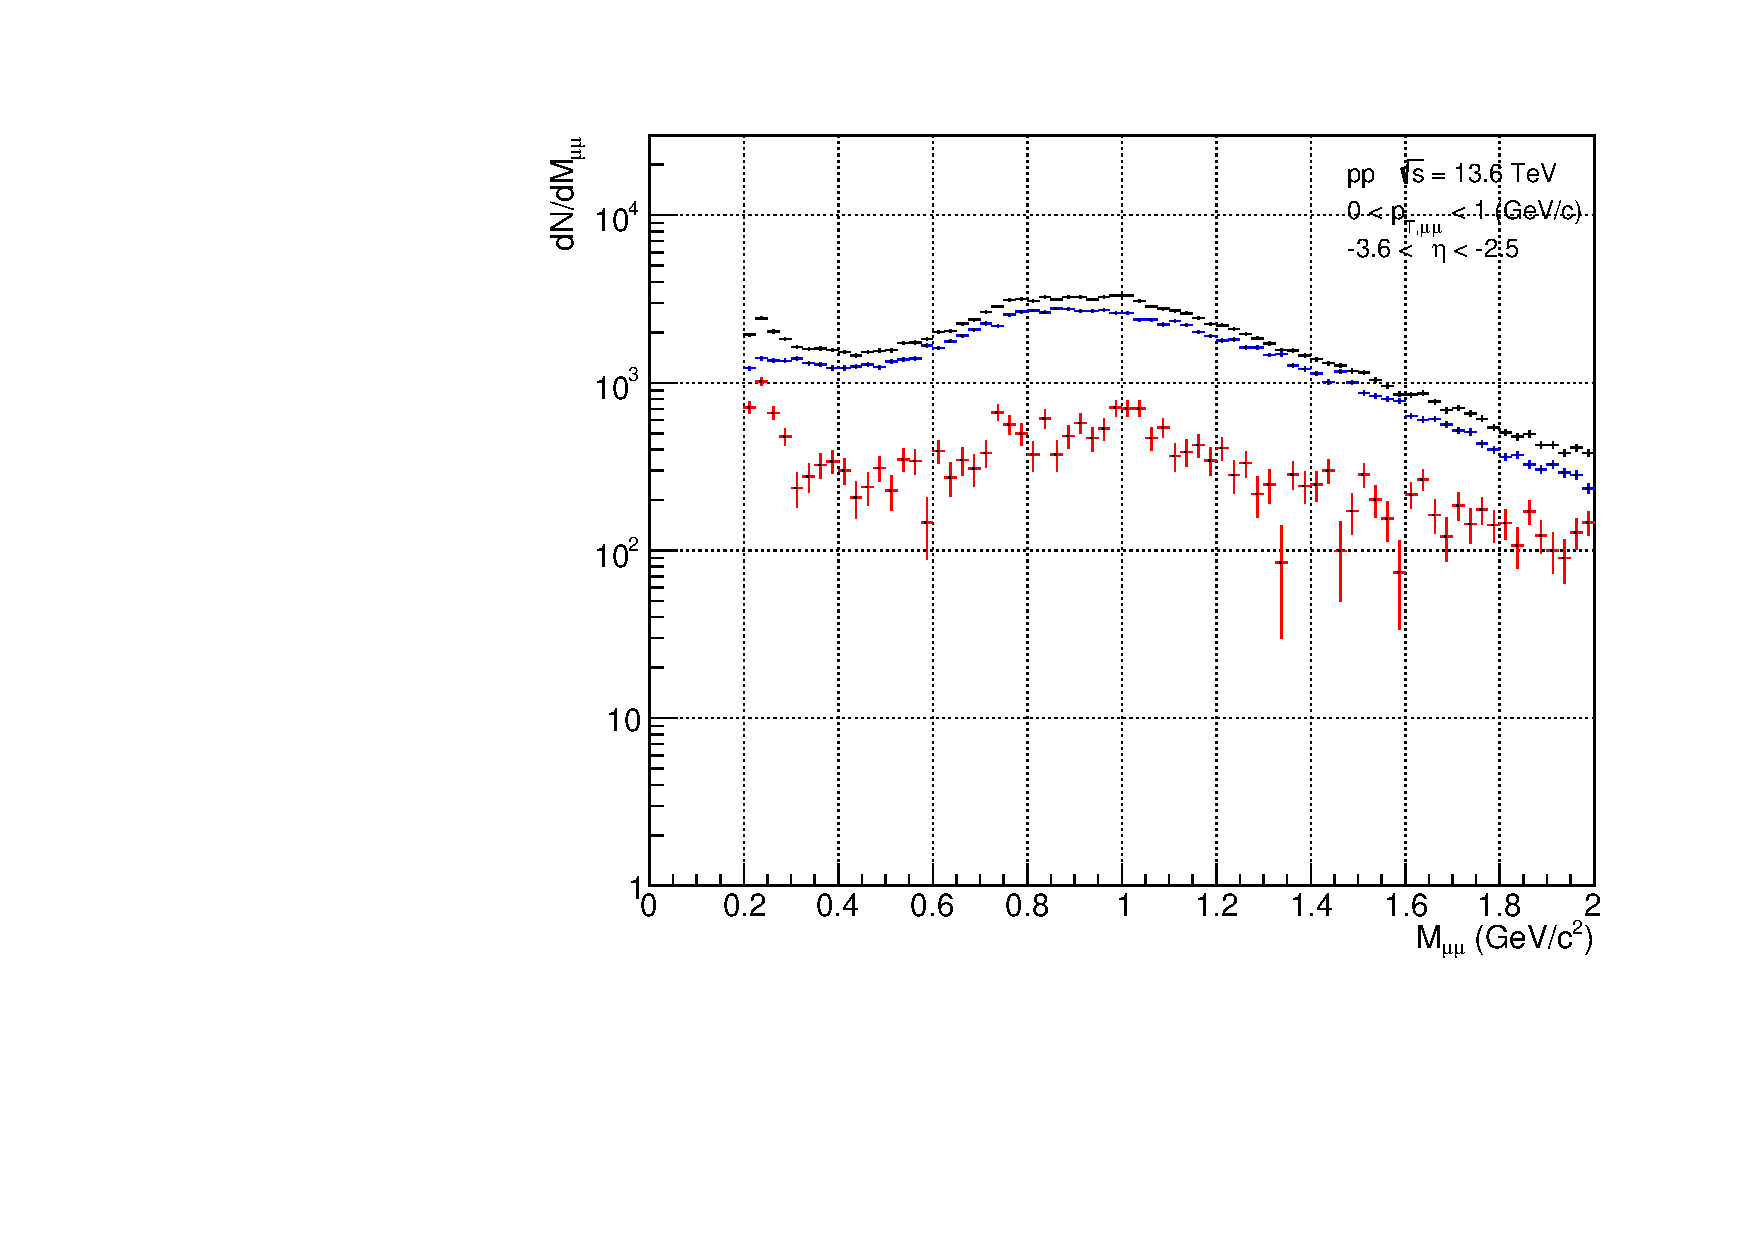
\includegraphics[keepaspectratio, scale=0.4]{fig/3_6_CB_pt0to1.pdf}
            \caption{Combinatorial subtraction of dimuon transverse momentum 0 < $p_T$ < 1}
            \label{Analysis:Dimuon:pt0to1}
        \end{figure}
        The mass distribution of dimuons with \( p_T \) below 1 GeV, not shown in \ref{Analysis:Dimuon:CB:CB_pt_separation}, is presented here.
        From \ref{Analysis:Dimuon:pt0to1}, the peak structures of \(\omega\) and \(\phi\) could not be measured. This is due to the insufficient reconstruction resolution of \(\eta\), \(p_T\), and \(\phi\) at low \(p_T\) for single muons. The introduction of the MFT is expected to enable high-precision measurements of \(\eta\) and \(\phi\), which would improve the reconstruction resolution of \(p_T\) through enhanced \(\eta\) and \(\phi\) resolution. However, with the current reconstruction method, sufficient resolution has not been achieved, resulting in the inability to observe the peaks of \(\omega\) and \(\phi\) in the dimuon invariant mass distribution at low transverse momentum. This can likely be attributed to issues in matching tracks from the newly introduced MFT and those from the MCH, which prevent achieving adequate resolution. This chapter presents an analysis to improve the MFT-MCH matching purity across all transverse momentum distributions without restricting to low \(p_T\).

        \subsubsection{MFT-MCH matching $\chi^2$ Optimization}
        \label{matching_chi2_opt}
            Using the yield analysis method for \(\omega \rightarrow \mu\mu, \phi \rightarrow \mu\mu\) described in \ref{Analysis:Dimuon:Combinatorial BG subtraction}-\ref{Analysis:Dimuon:Yieldcal}, the MFT-MCH matching \(\chi^2\) cut value for single muon tracks was optimised to maximise signal detection efficiency. The MFT-MCH matching \(\chi^2\) value represents the parameter difference when extrapolating MFT and MCH tracks to the matching plane. A larger \(\chi^2\) value indicates more fake matches, whereas a smaller value corresponds to more correct matches. Fake match tracks can be removed by applying a cut on this value. However, optimising the cut to minimise fake matches while preserving as many correct matches as possible is necessary. In this study, the optimisation was performed by maximising the signal significance using the peaks of \(\omega\) and \(\phi\).
            The signal was calculated by performing the same analysis as in \ref{Analysis:Dimuon:Combinatorial BG subtraction}, \ref{Peak_extraction}, and \ref{Analysis:Dimuon:Yieldcal} for the mass distributions in all transverse momentum regions. The number of background events was determined by counting the entries in the background-subtracted mass distribution within the same mass window used for signal calculation, and this was used as the background estimate. The significance, \( S/\sqrt{S+BG} \), was then calculated. This calculation was performed for mass distributions reconstructed using only muons with an MFT-MCH matching \(\chi^2\) below a given threshold.  
            Figure \ref{Analysis:Dimuon:Matching_CB} presents the results of the combinatorial background subtraction after applying the \(\chi^2\) cut. Similar to \ref{Analysis:Dimuon:CB:CB_pt_separation}, the black histogram represents the mass distribution reconstructed from all oppositely charged muon pairs in the same event. The blue histogram represents the combinatorial background estimated using the Like Sign method. The red histogram corresponds to the background-subtracted distribution, representing the invariant mass distribution of correlated dimuons.
            \begin{figure}[H]
                \centering
                \begin{minipage}{0.45\textwidth}
                    \centering
                    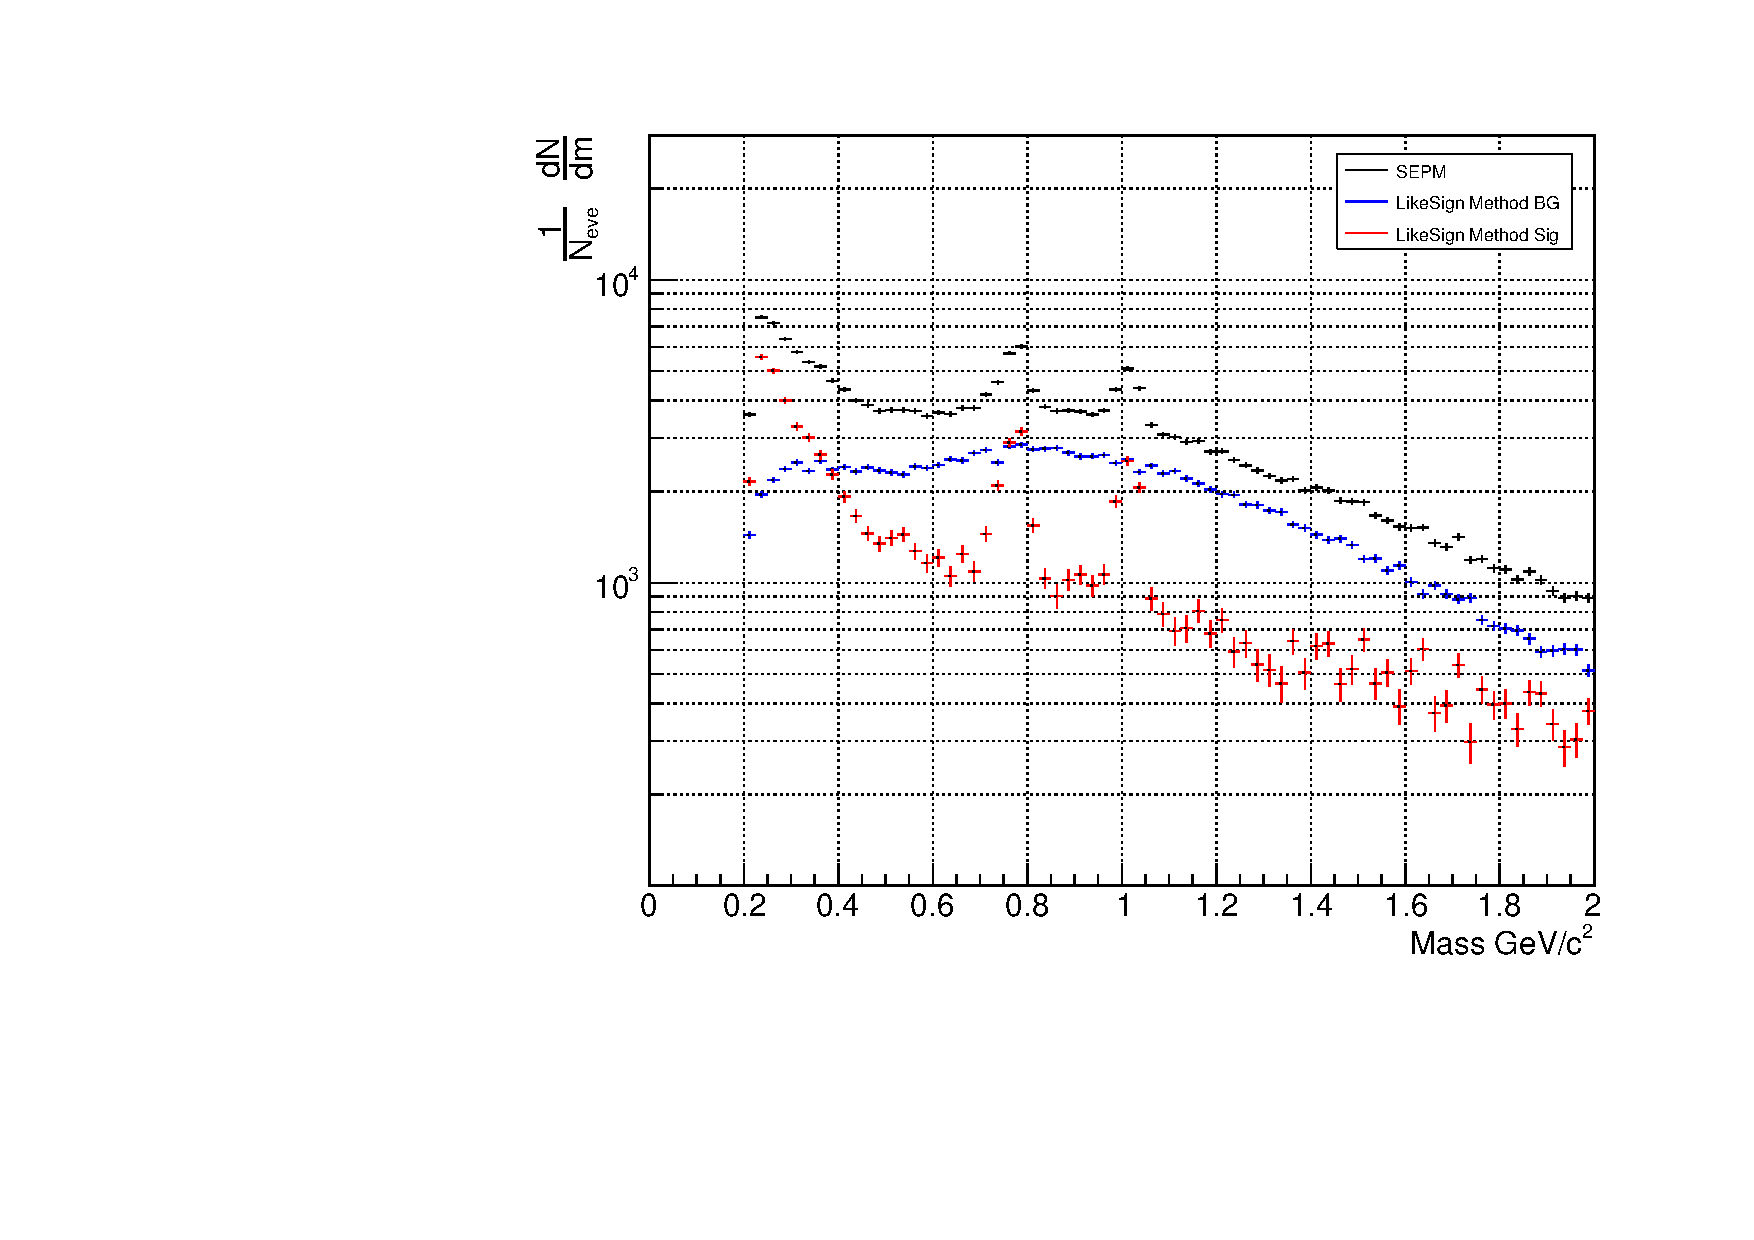
\includegraphics[width=\textwidth]{fig/3_4_4_CB_chi2_20.pdf}
                    \caption*{MFT-MCH matching $\chi^2 < 20$}
                \end{minipage}
                \hfill
                \begin{minipage}{0.45\textwidth}
                    \centering
                    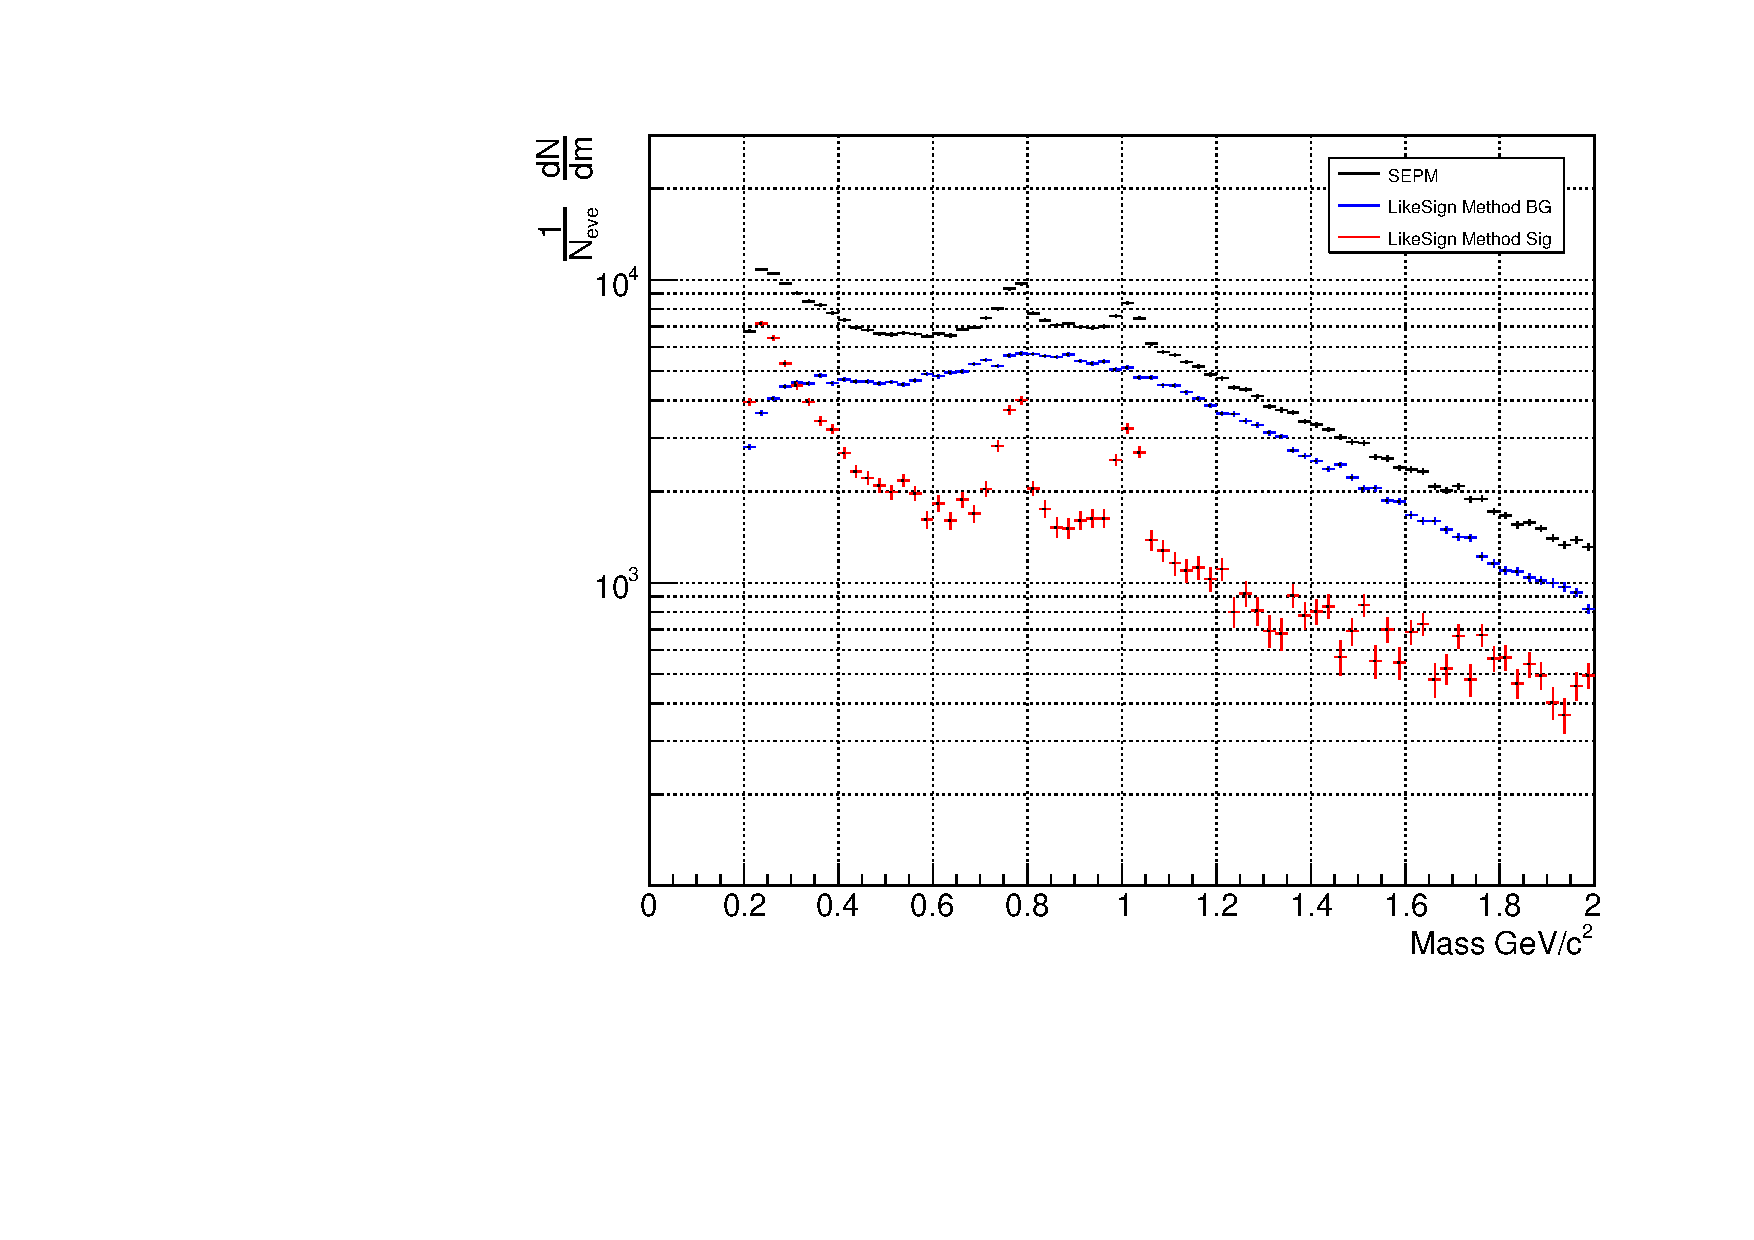
\includegraphics[width=\textwidth]{fig/3_4_4_CB_chi2_40.pdf}
                    \caption*{MFT-MCH matching $\chi^2 < 40$}
                \end{minipage}
                \\
                \vspace{1em}
                \begin{minipage}{0.45\textwidth}
                    \centering
                    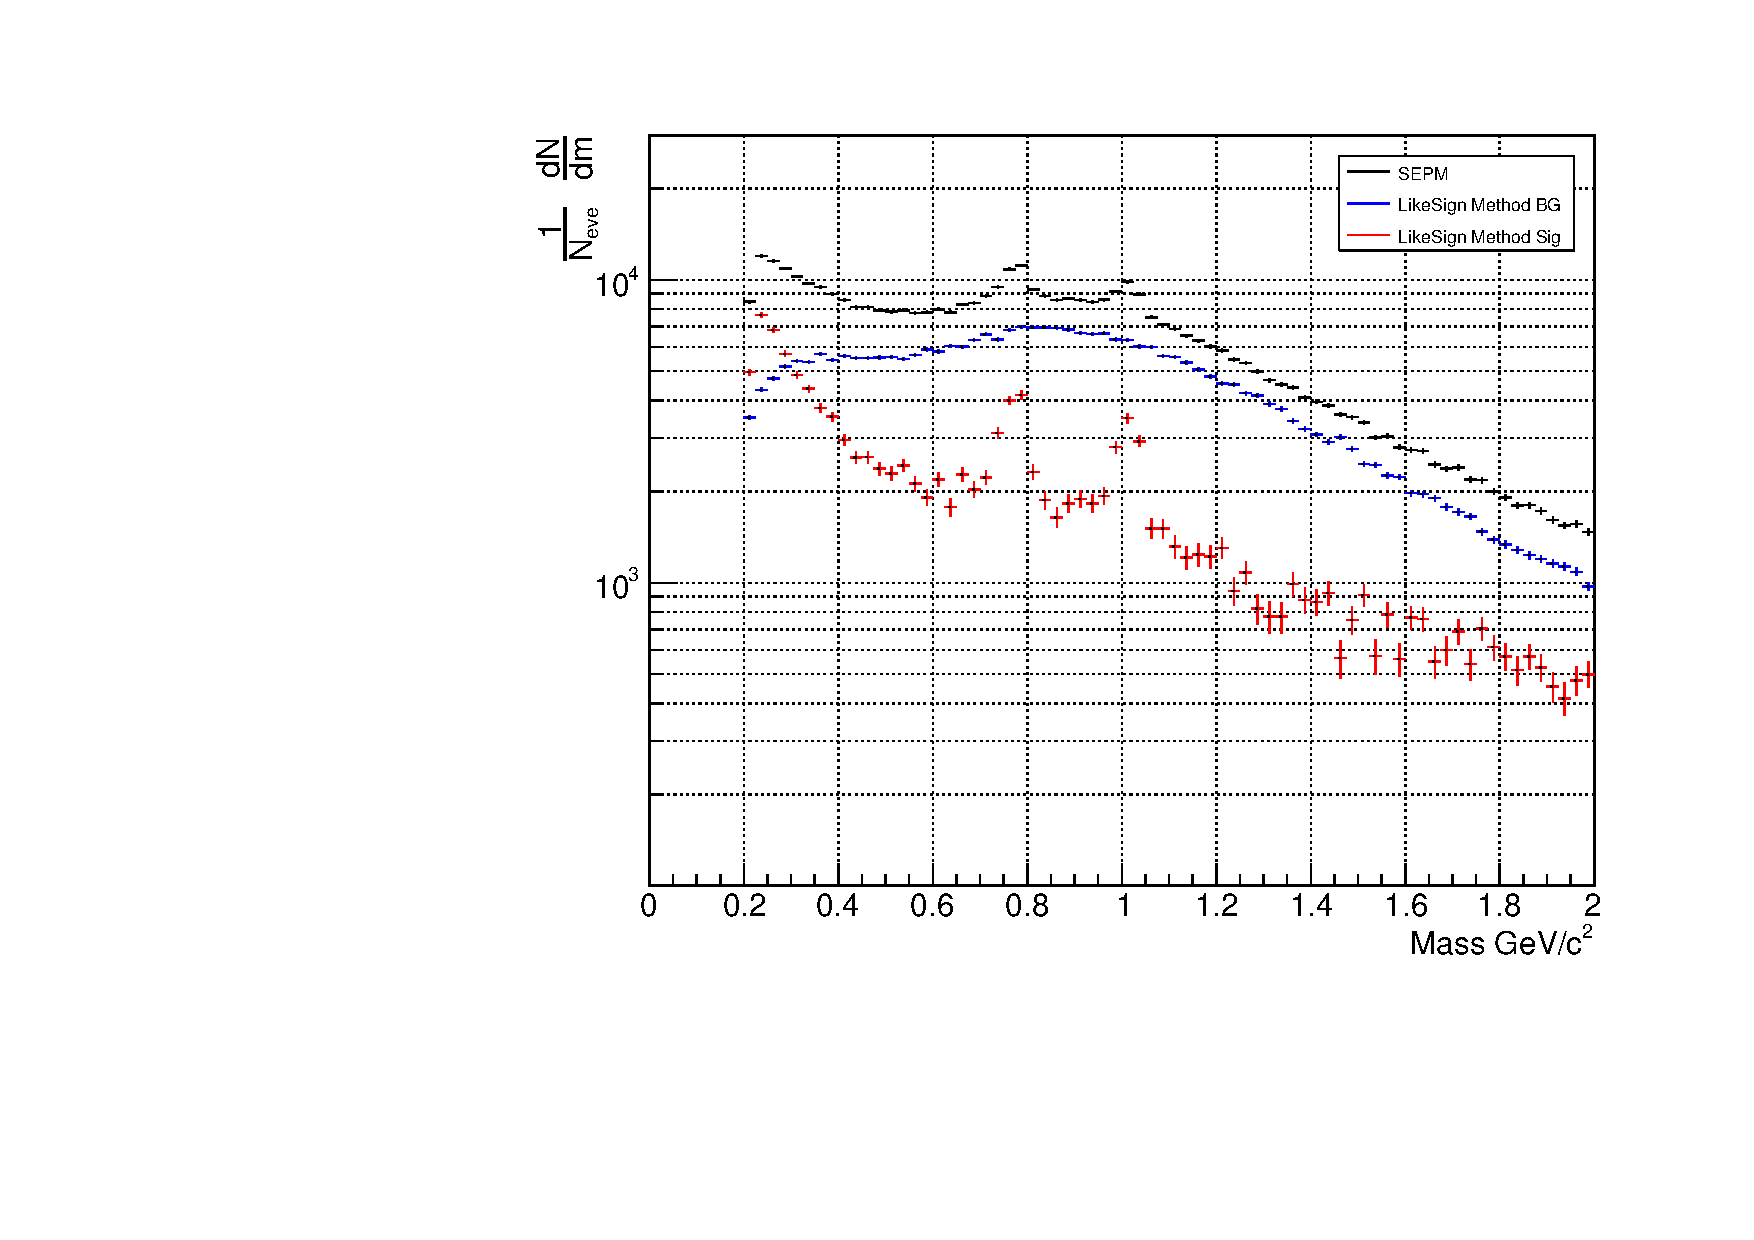
\includegraphics[width=\textwidth]{fig/3_4_4_CB_chi2_60.pdf}
                    \caption*{MFT-MCH matching $\chi^2 < 60$}
                \end{minipage}
                \hfill
                \begin{minipage}{0.45\textwidth}
                    \centering
                    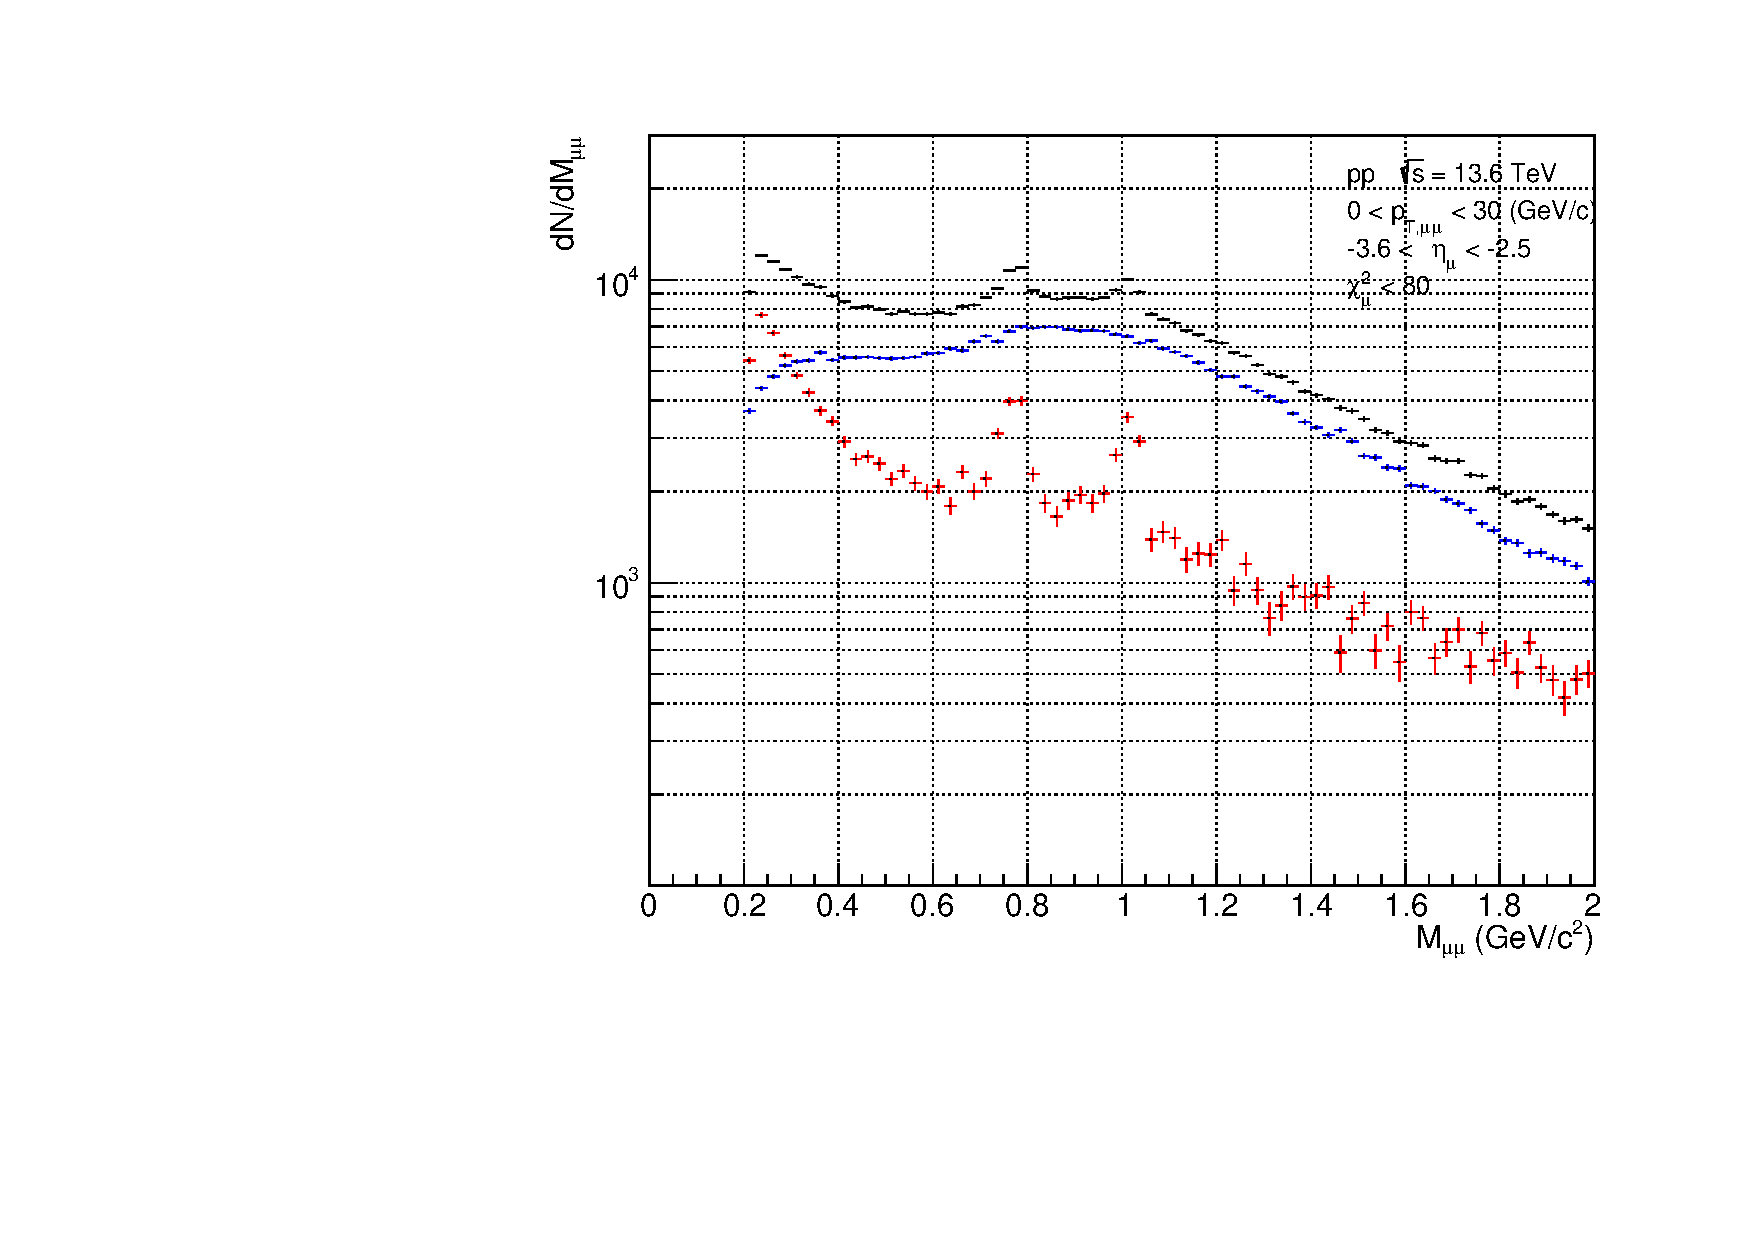
\includegraphics[width=\textwidth]{fig/3_4_4_CB_chi2_80.pdf}
                    \caption*{MFT-MCH matching $\chi^2 < 80$} 
             
                \end{minipage}
                \\
                \vspace{1em}
                \begin{minipage}{0.45\textwidth}
                    \centering
                    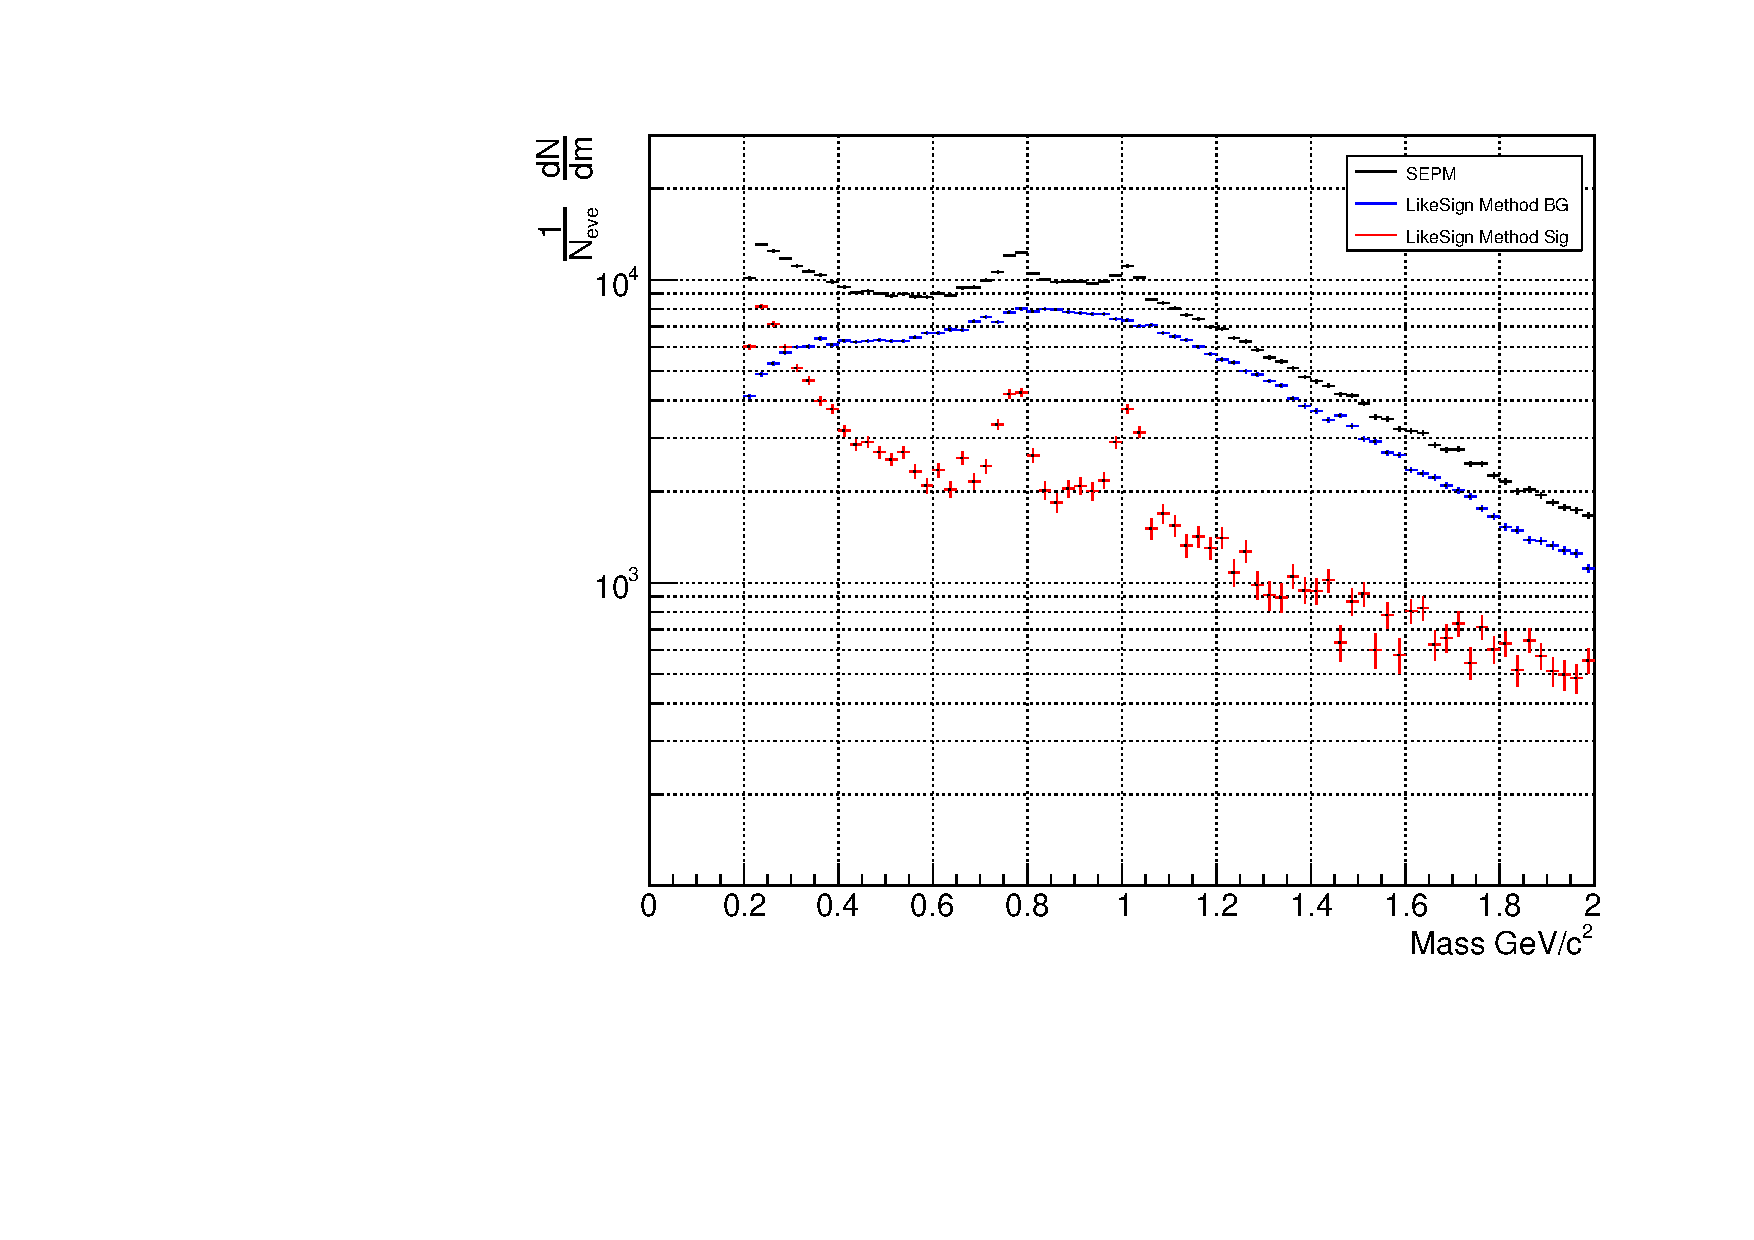
\includegraphics[width=\textwidth]{fig/3_4_4_CB_chi2_100.pdf}
                    \caption*{MFT-MCH matching $\chi^2 < 100$}
                \end{minipage}
                \hfill
                \begin{minipage}{0.45\textwidth}
                    \centering
                    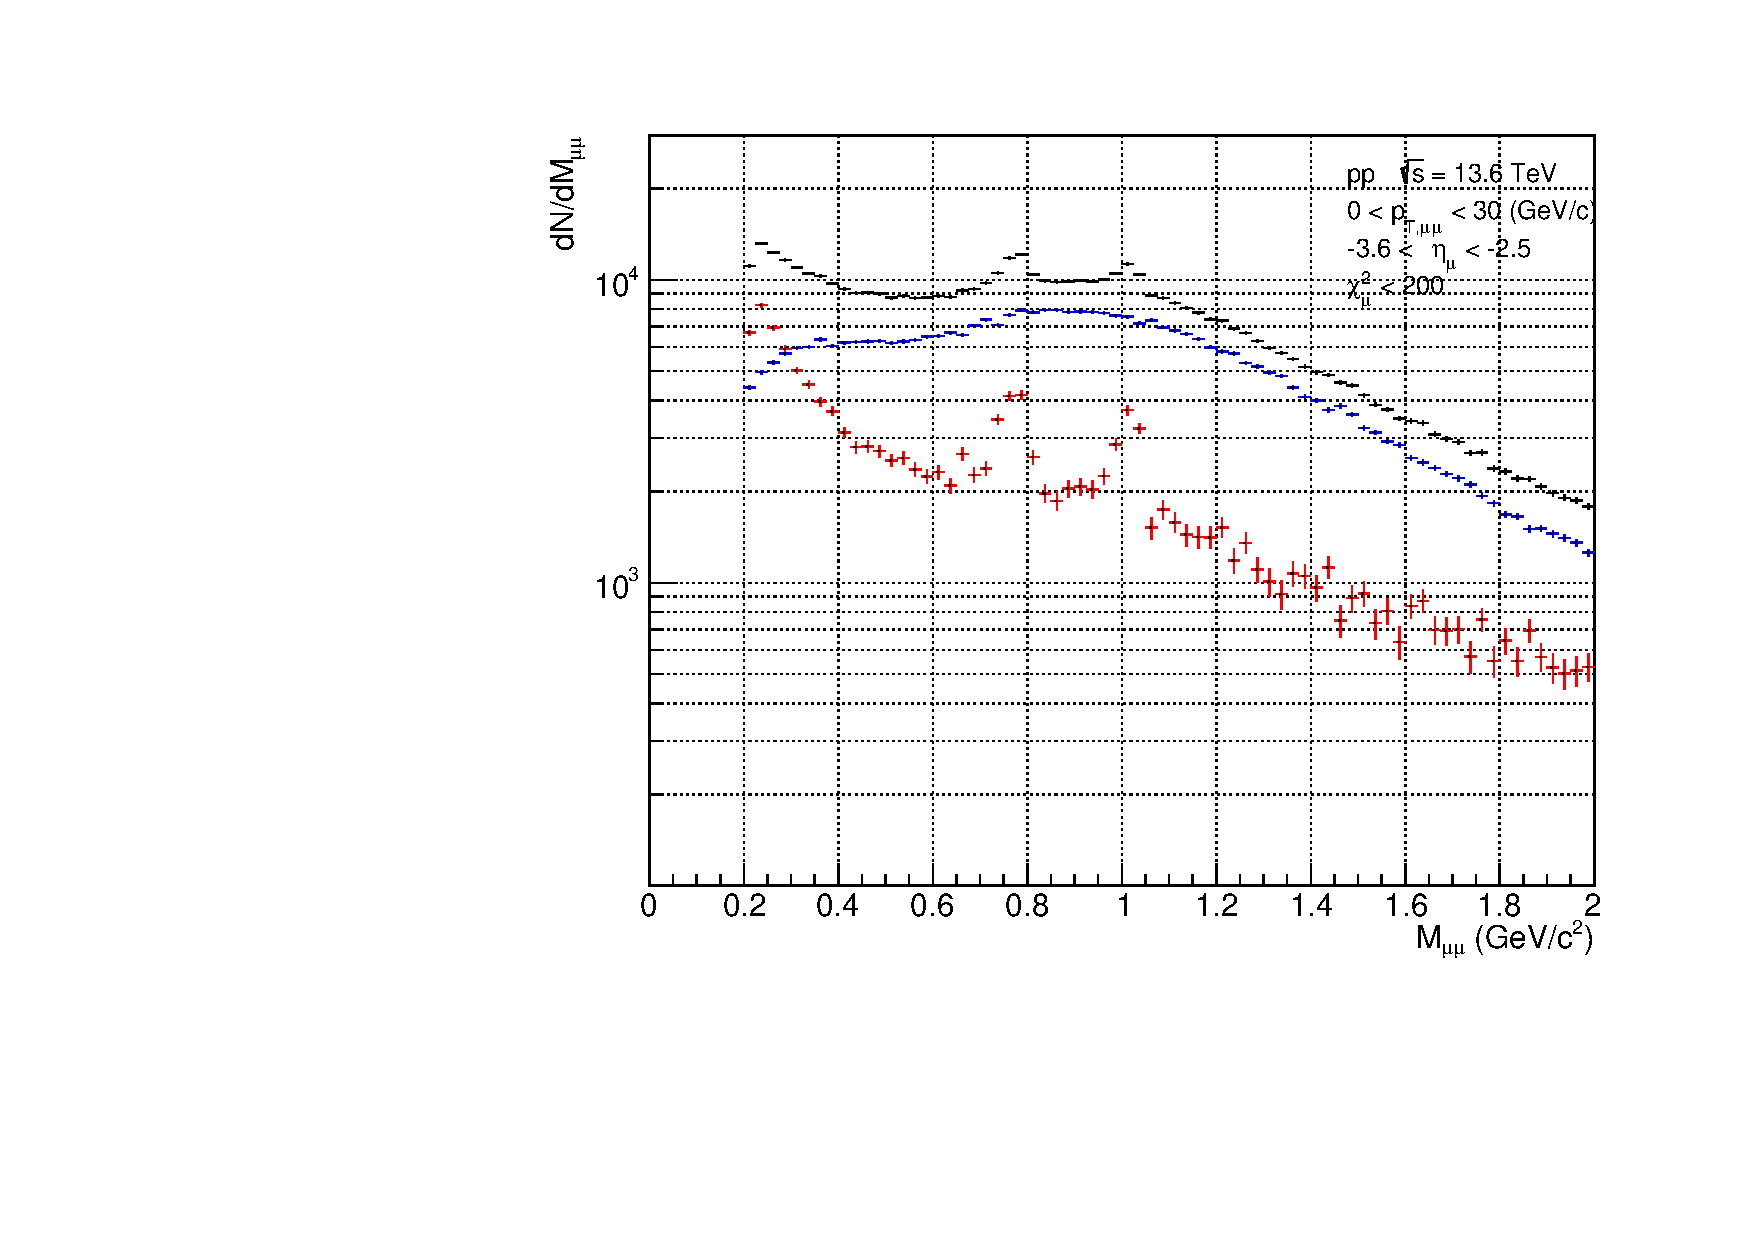
\includegraphics[width=\textwidth]{fig/3_4_4_CB_chi2_200.pdf}
                    \caption*{MFT-MCH matching $\chi^2 < 200$}
                \end{minipage}
                \caption{The result of Combinatorial Background subtraction after applying the MFT-MCH matching $\chi^2$ cut}
                \label{Analysis:Dimuon:Matching_CB}
            \end{figure}
            The black distribution decreases in size by reducing the \(\chi^2\) cut. Additionally, it can be observed that the \(\omega\) and \(\phi\) peaks in the red distribution become more pronounced. Figure \ref{Analysis:Dimuon:Matching_Fit} shows the fitting results for this red distribution.
            \begin{figure}[H]
                \centering
                \begin{minipage}{0.45\textwidth}  
                    \centering
                    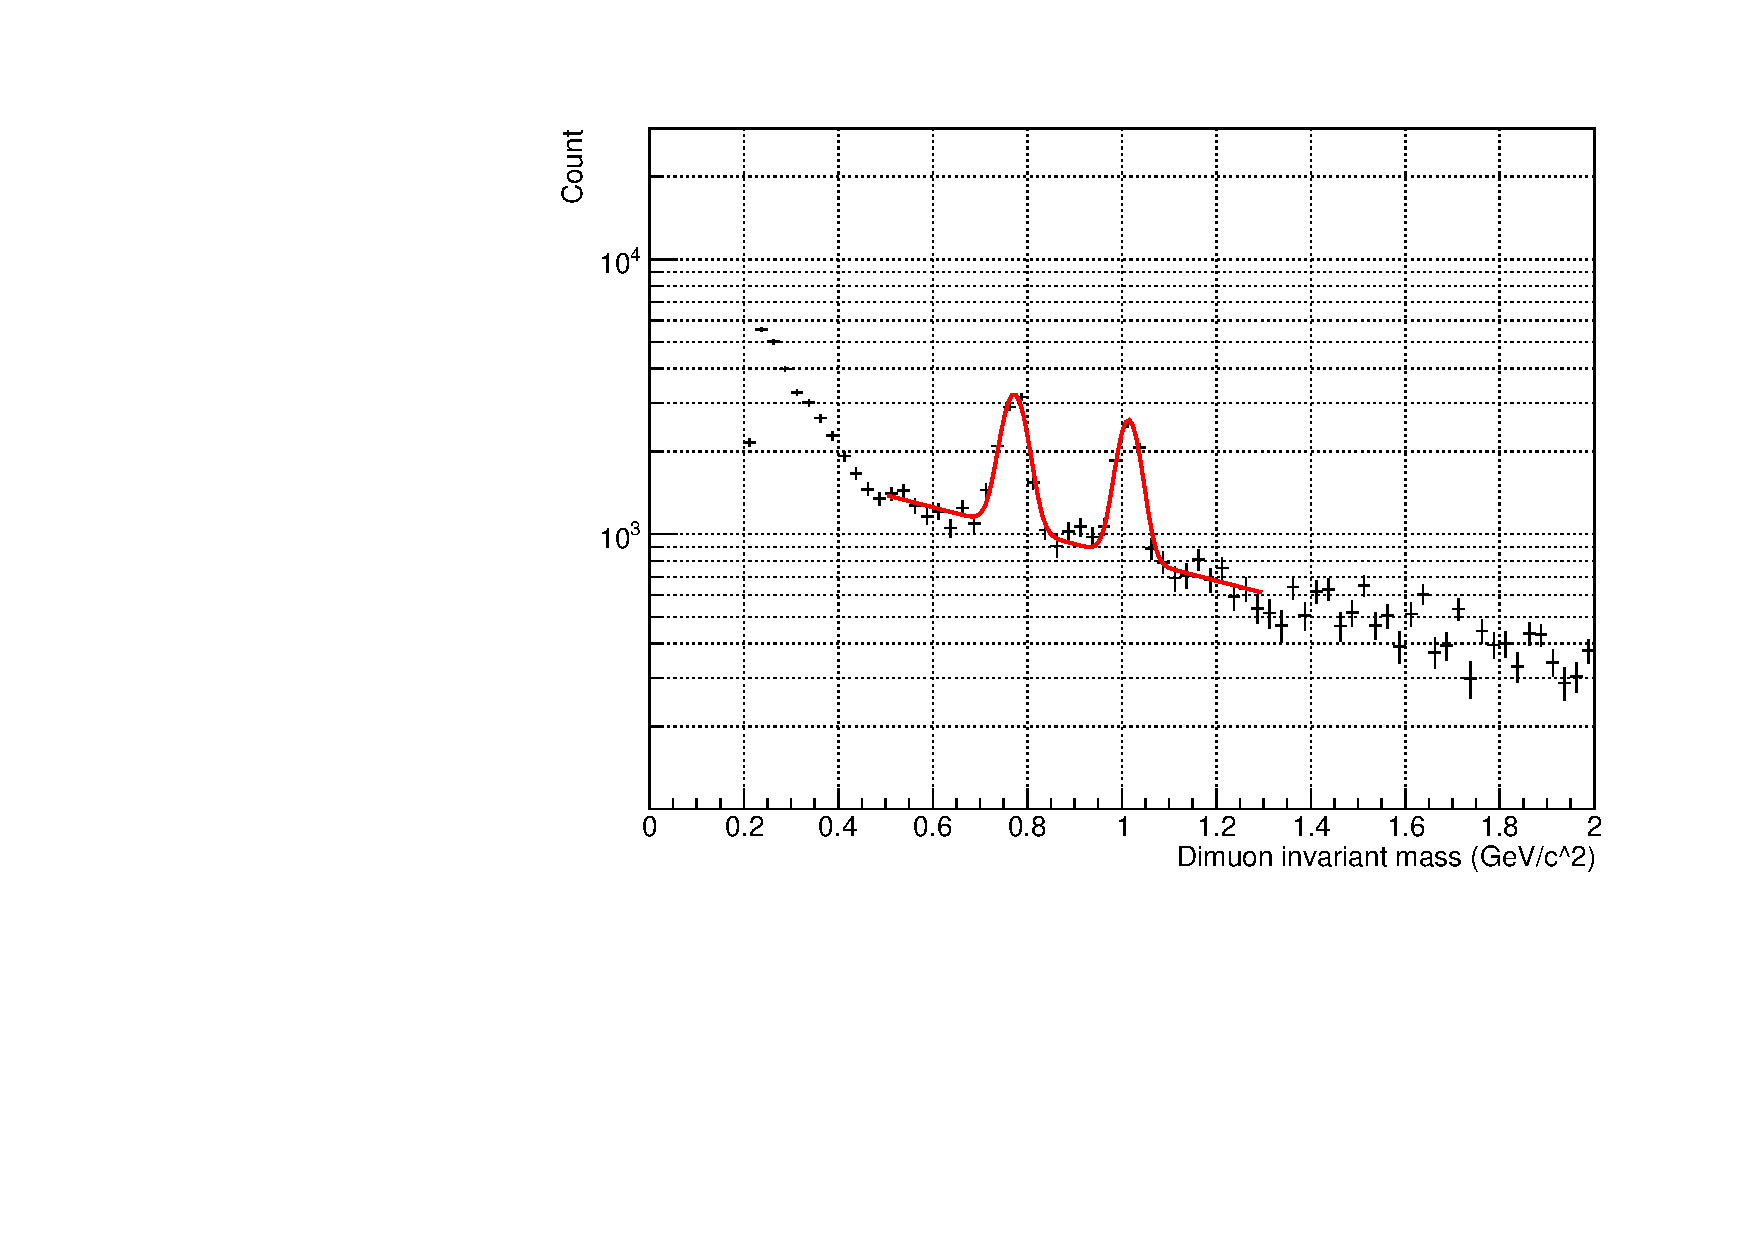
\includegraphics[width=\textwidth]{fig/3_4_4_Fit_chi2_20.pdf}
                    \caption*{MFT-MCH matching $\chi^2 < 20$}
                \end{minipage}
                \hfill
                \begin{minipage}{0.45\textwidth}
                    \centering
                    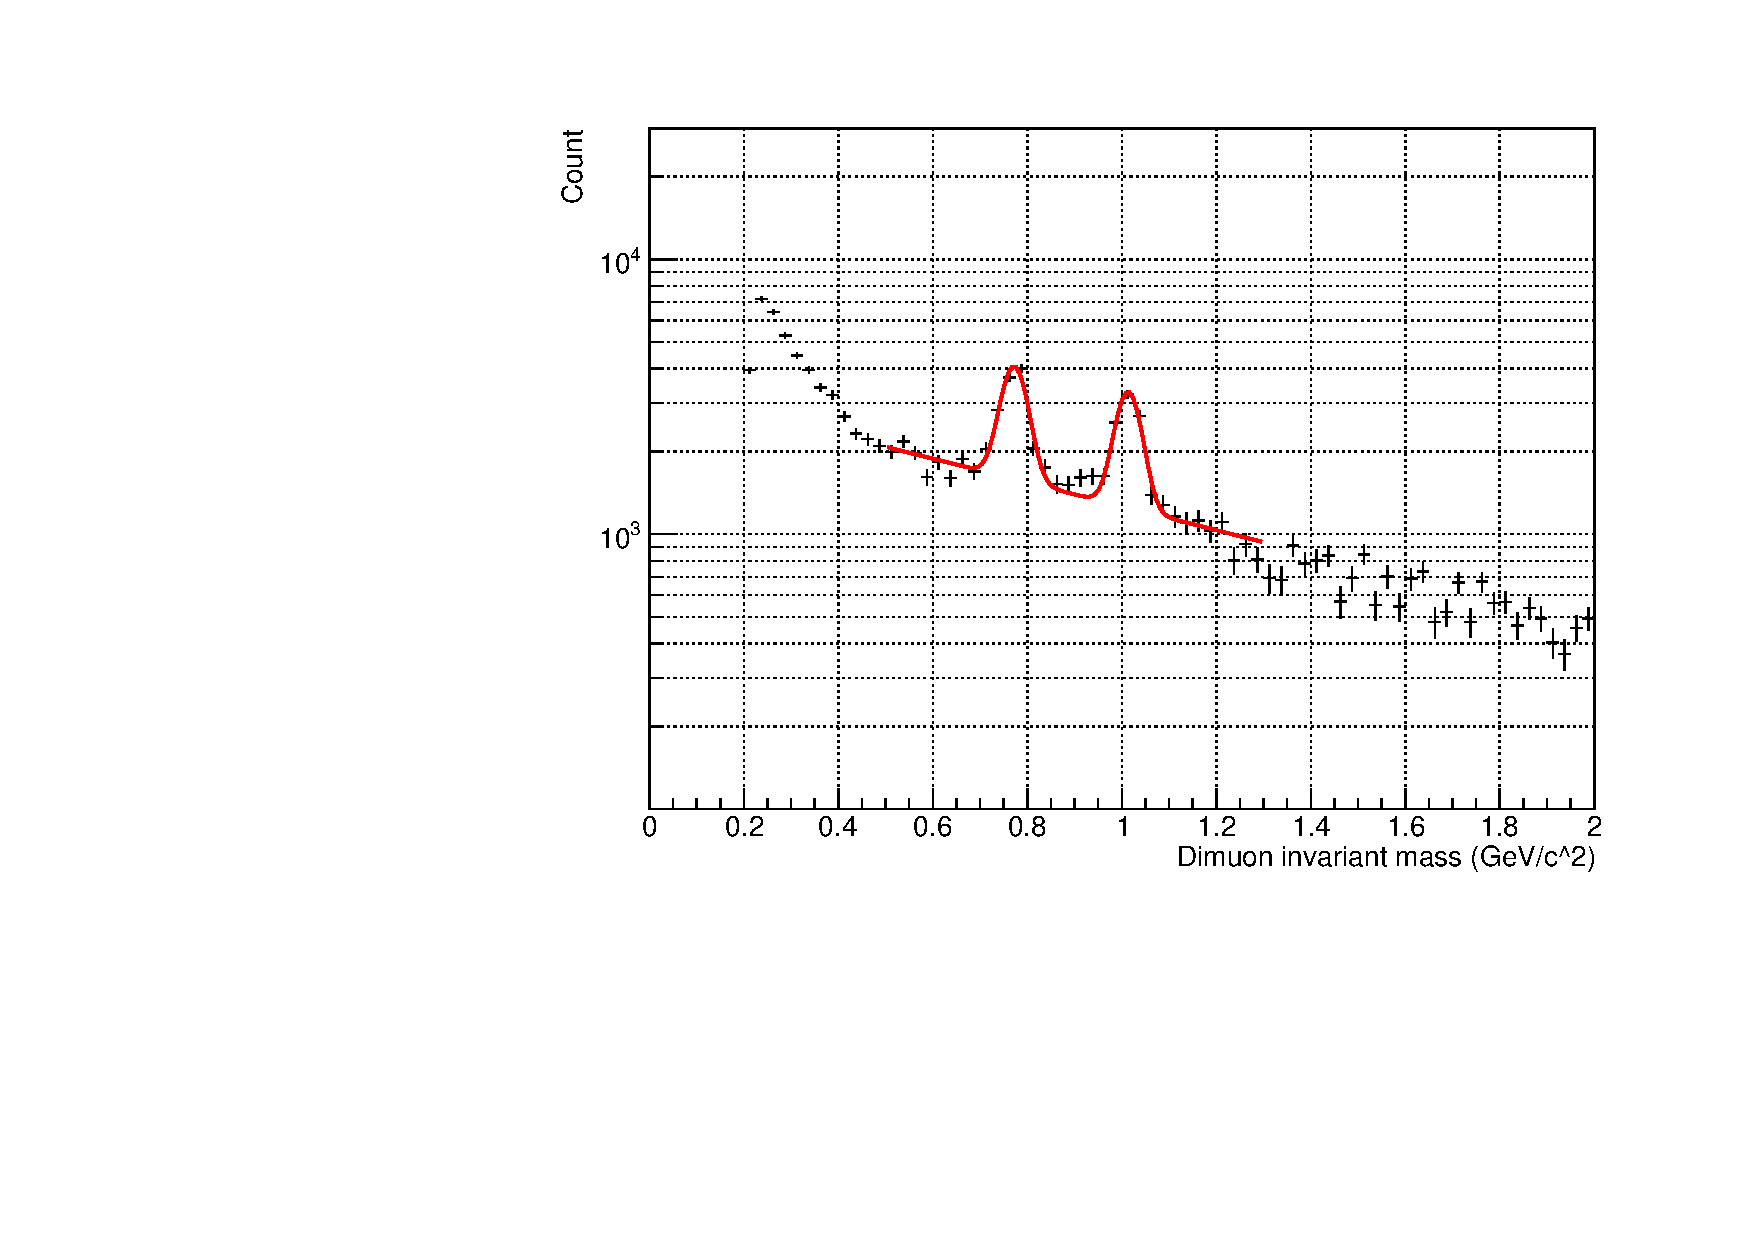
\includegraphics[width=\textwidth]{fig/3_4_4_Fit_chi2_40.pdf}
                    \caption*{MFT-MCH matching $\chi^2 < 40$}
                \end{minipage}
                \\
                \vspace{1em}
                \begin{minipage}{0.45\textwidth}
                    \centering
                    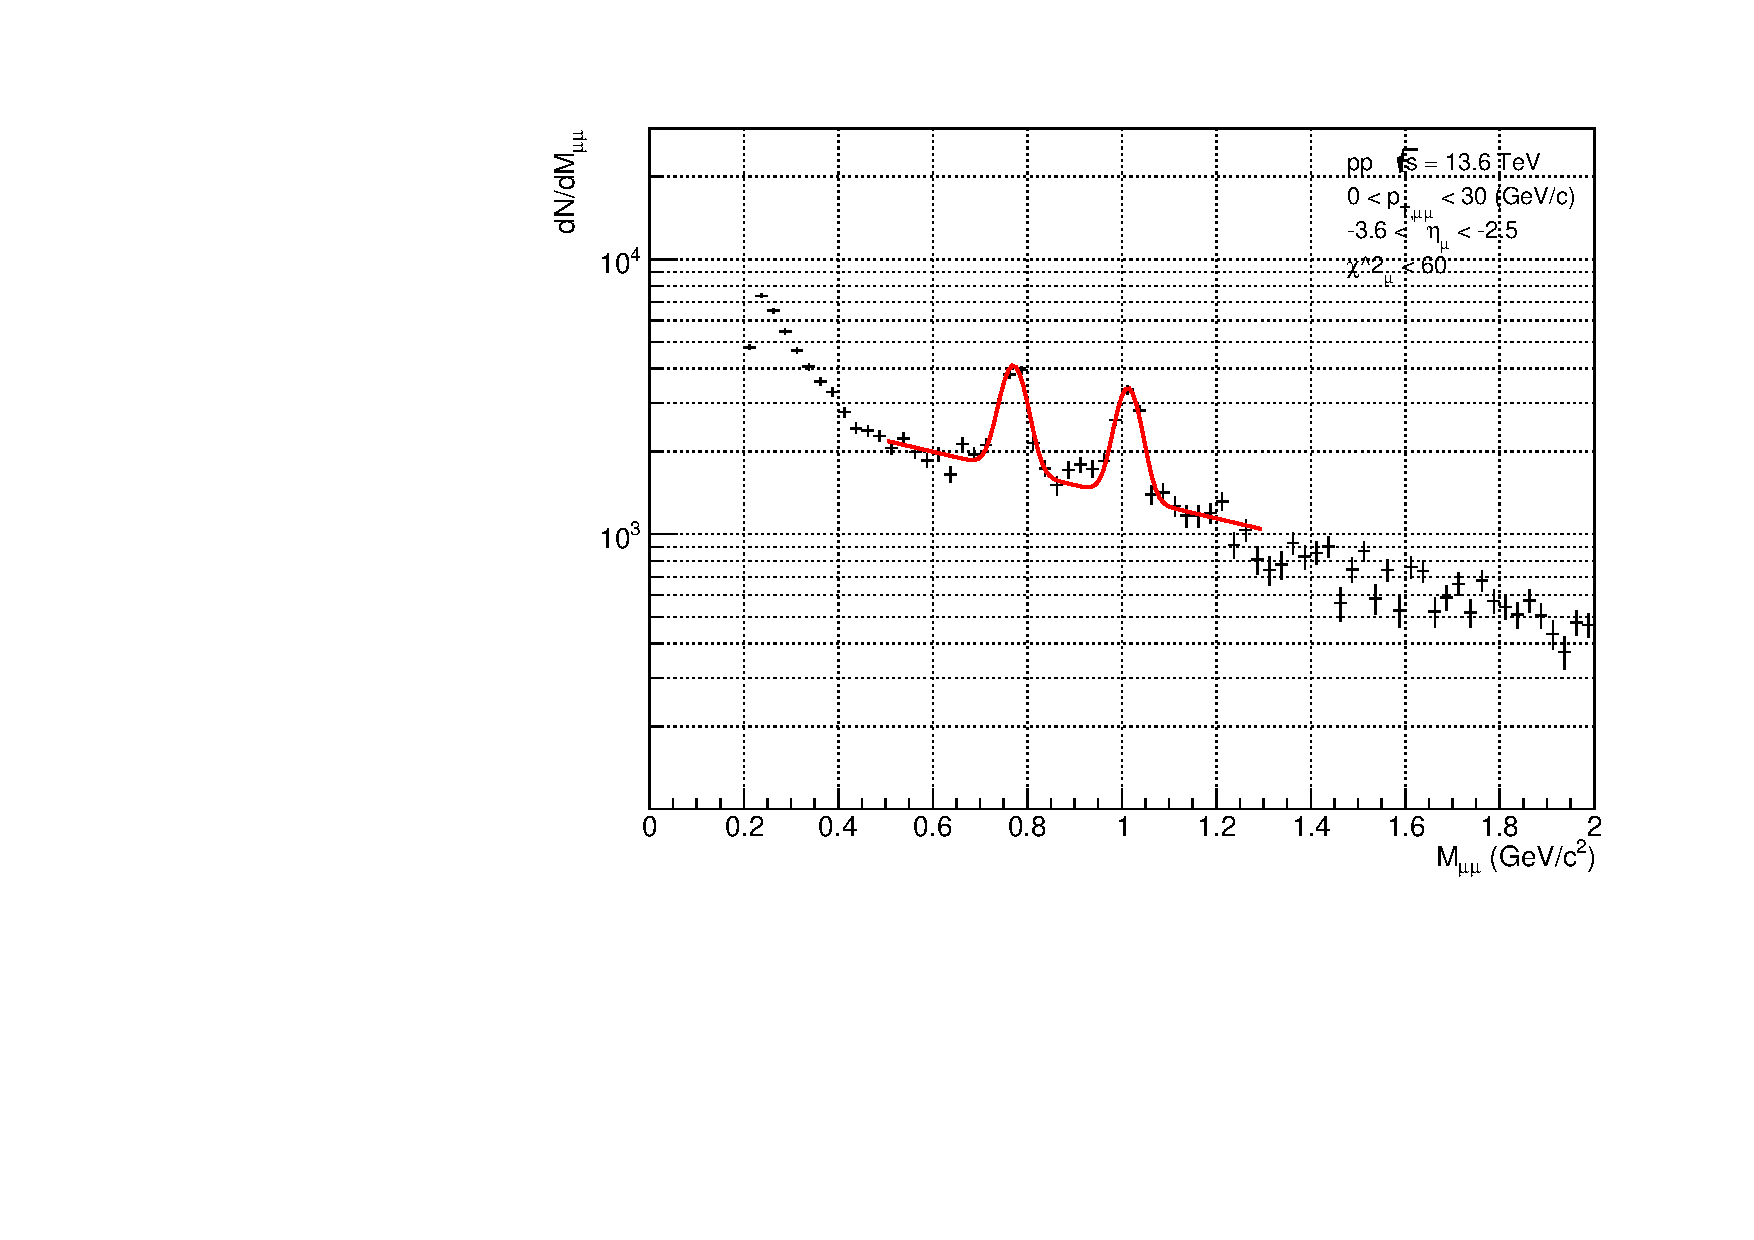
\includegraphics[width=\textwidth]{fig/3_4_4_Fit_chi2_60.pdf}
                    \caption*{MFT-MCH matching $\chi^2 < 60$}
                \end{minipage}
                \hfill
                \begin{minipage}{0.45\textwidth}
                    \centering
                    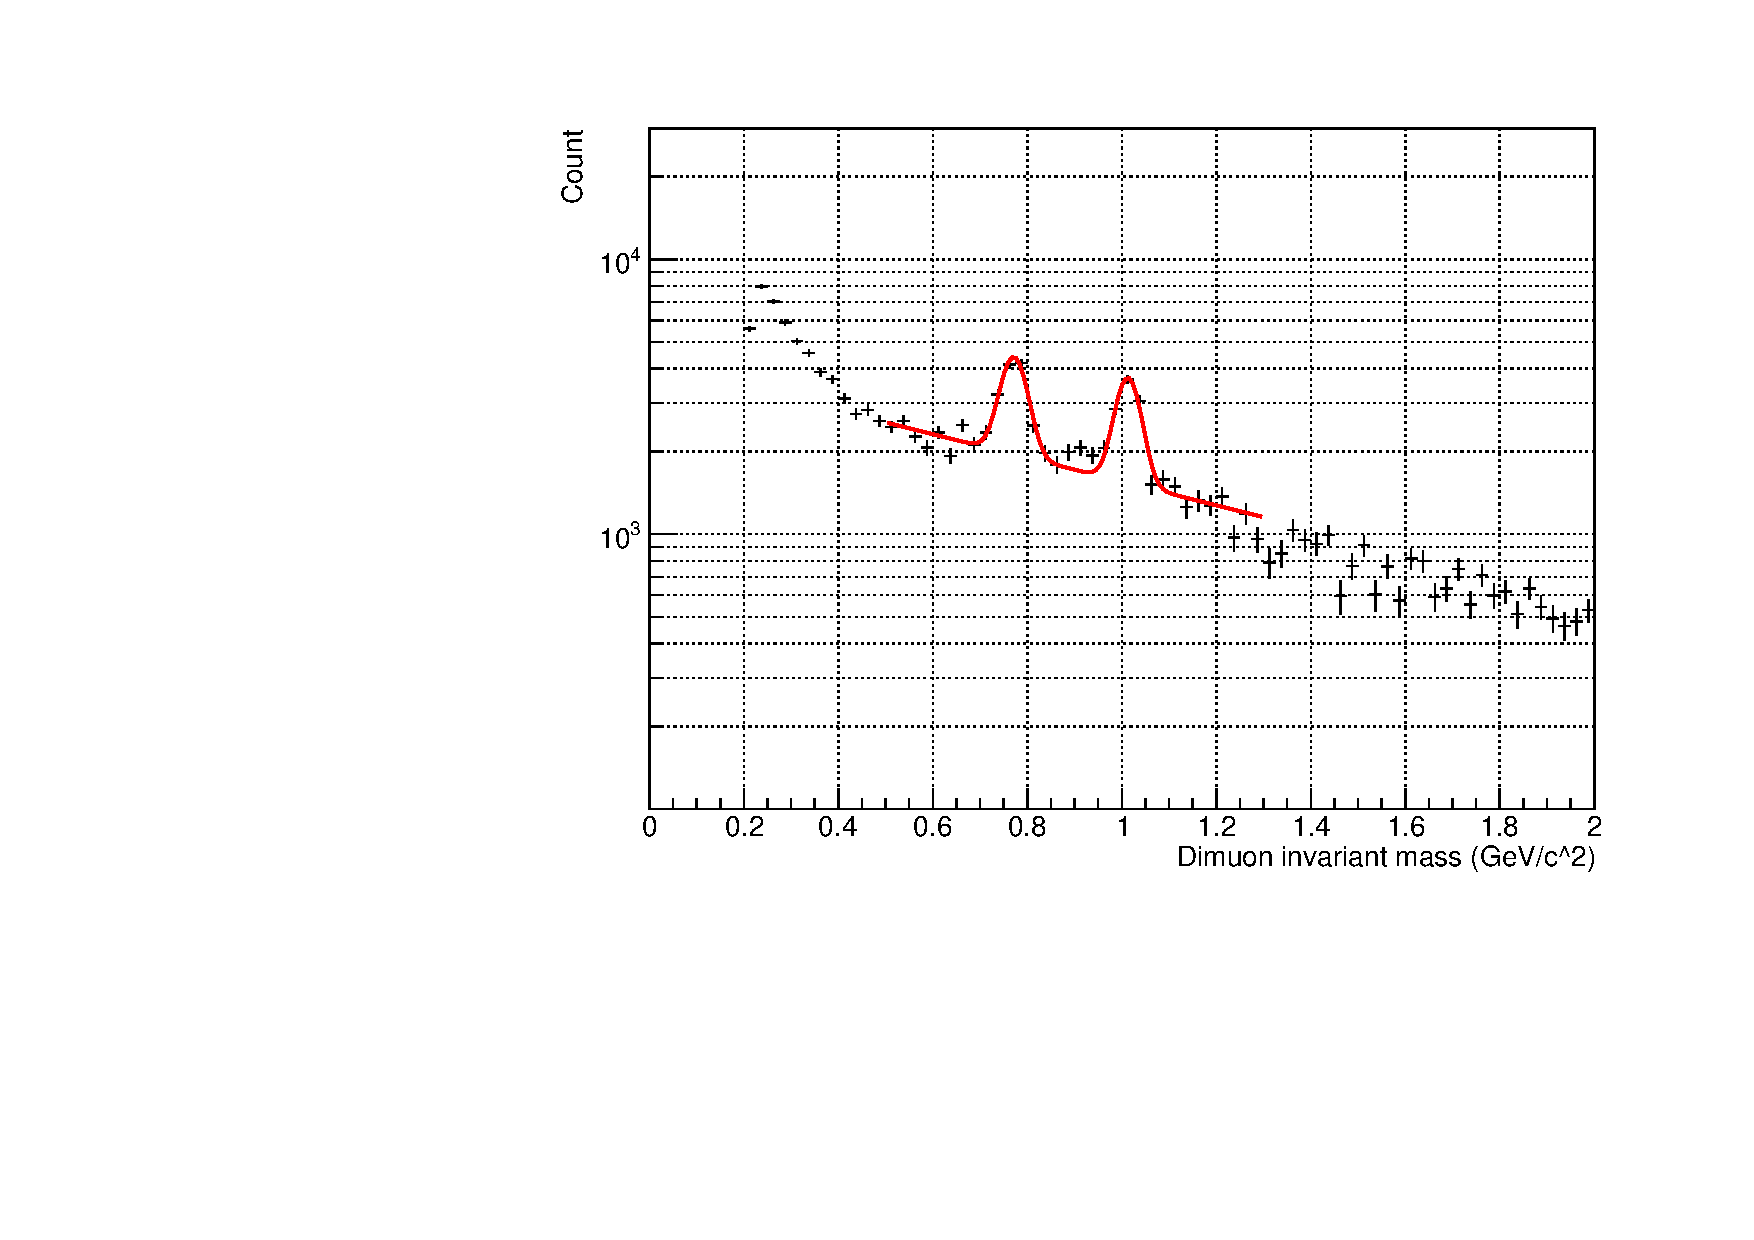
\includegraphics[width=\textwidth]{fig/3_4_4_Fit_chi2_80.pdf}
                    \caption*{MFT-MCH matching $\chi^2 < 80$} 
                \end{minipage}
                \\
                \vspace{1em}
                \begin{minipage}{0.45\textwidth}
                    \centering
                    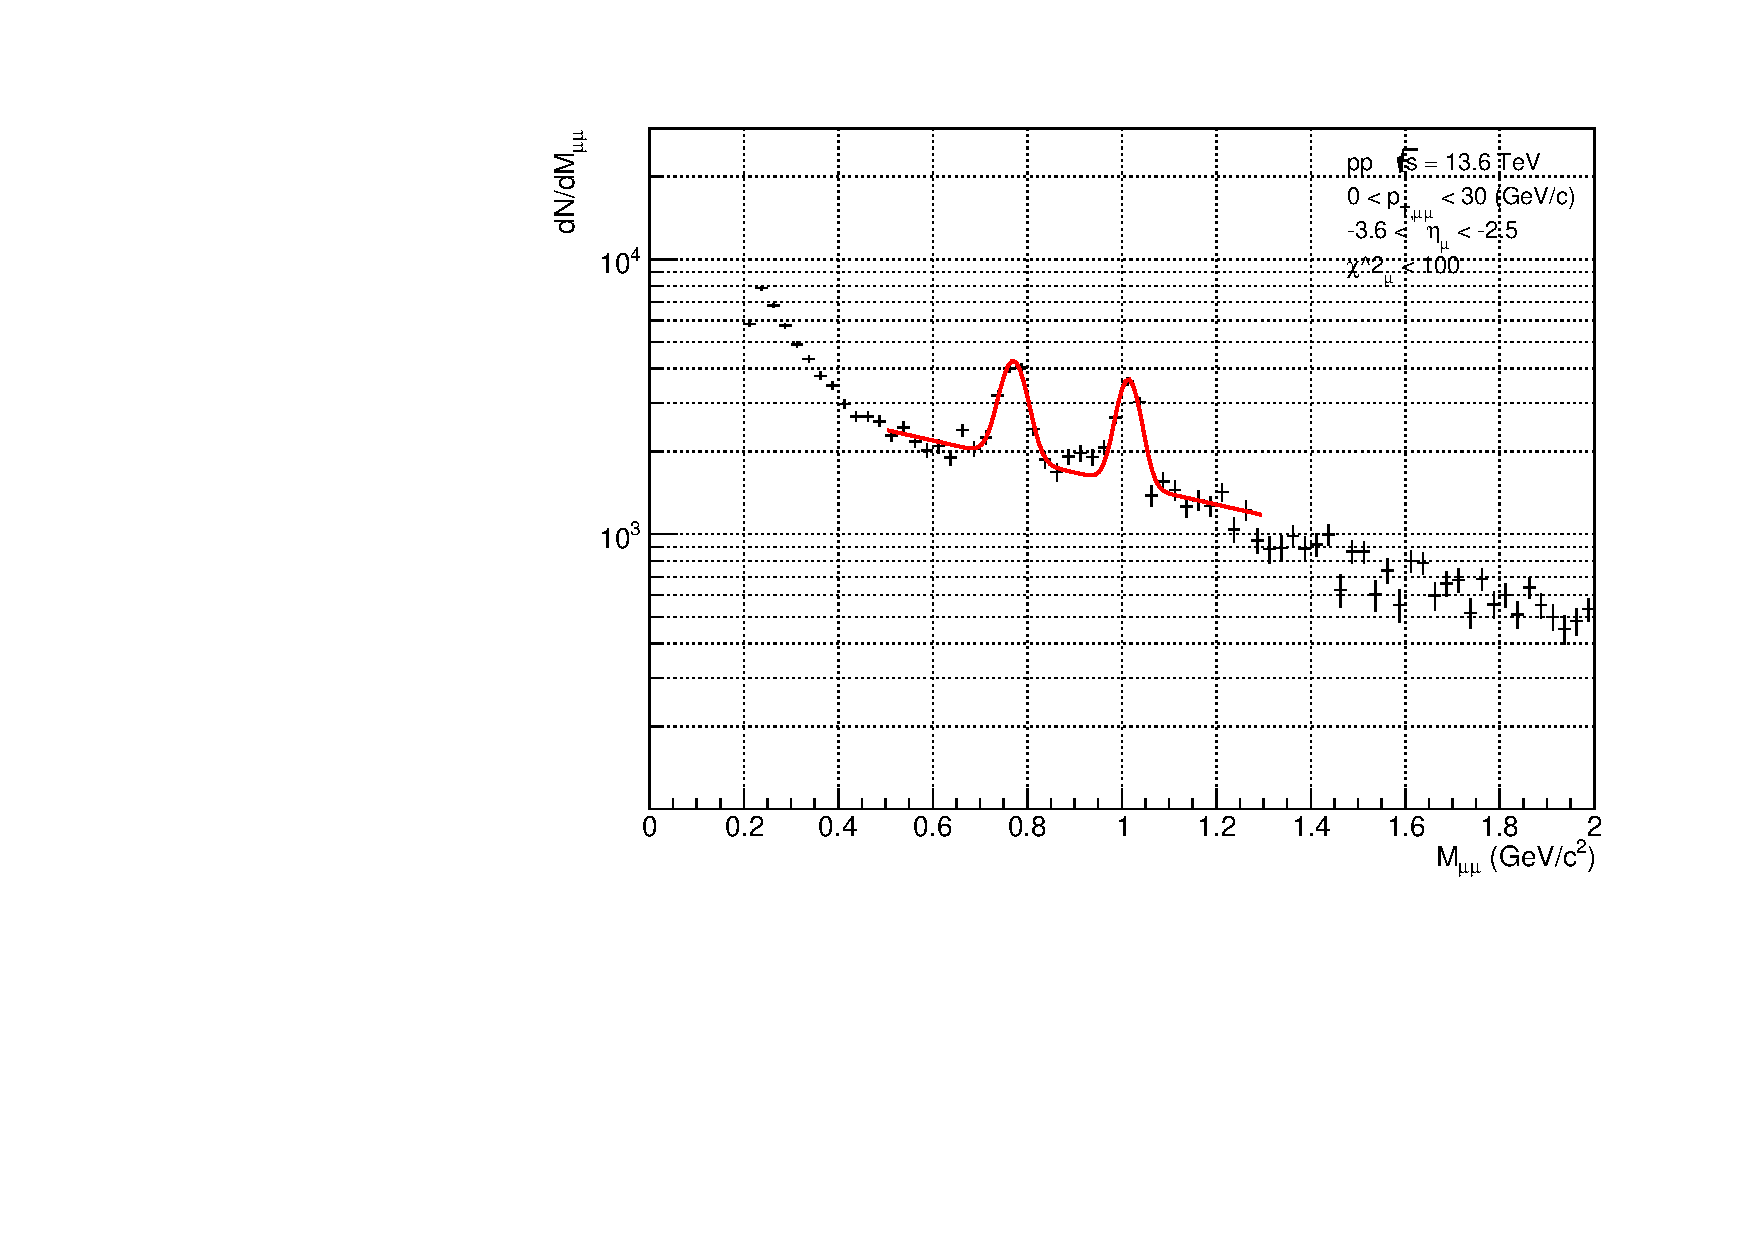
\includegraphics[width=\textwidth]{fig/3_4_4_Fit_chi2_100.pdf}
                    \caption*{MFT-MCH matching $\chi^2 < 100$}
                \end{minipage}
                \hfill
                \begin{minipage}{0.45\textwidth}
                    \centering
                    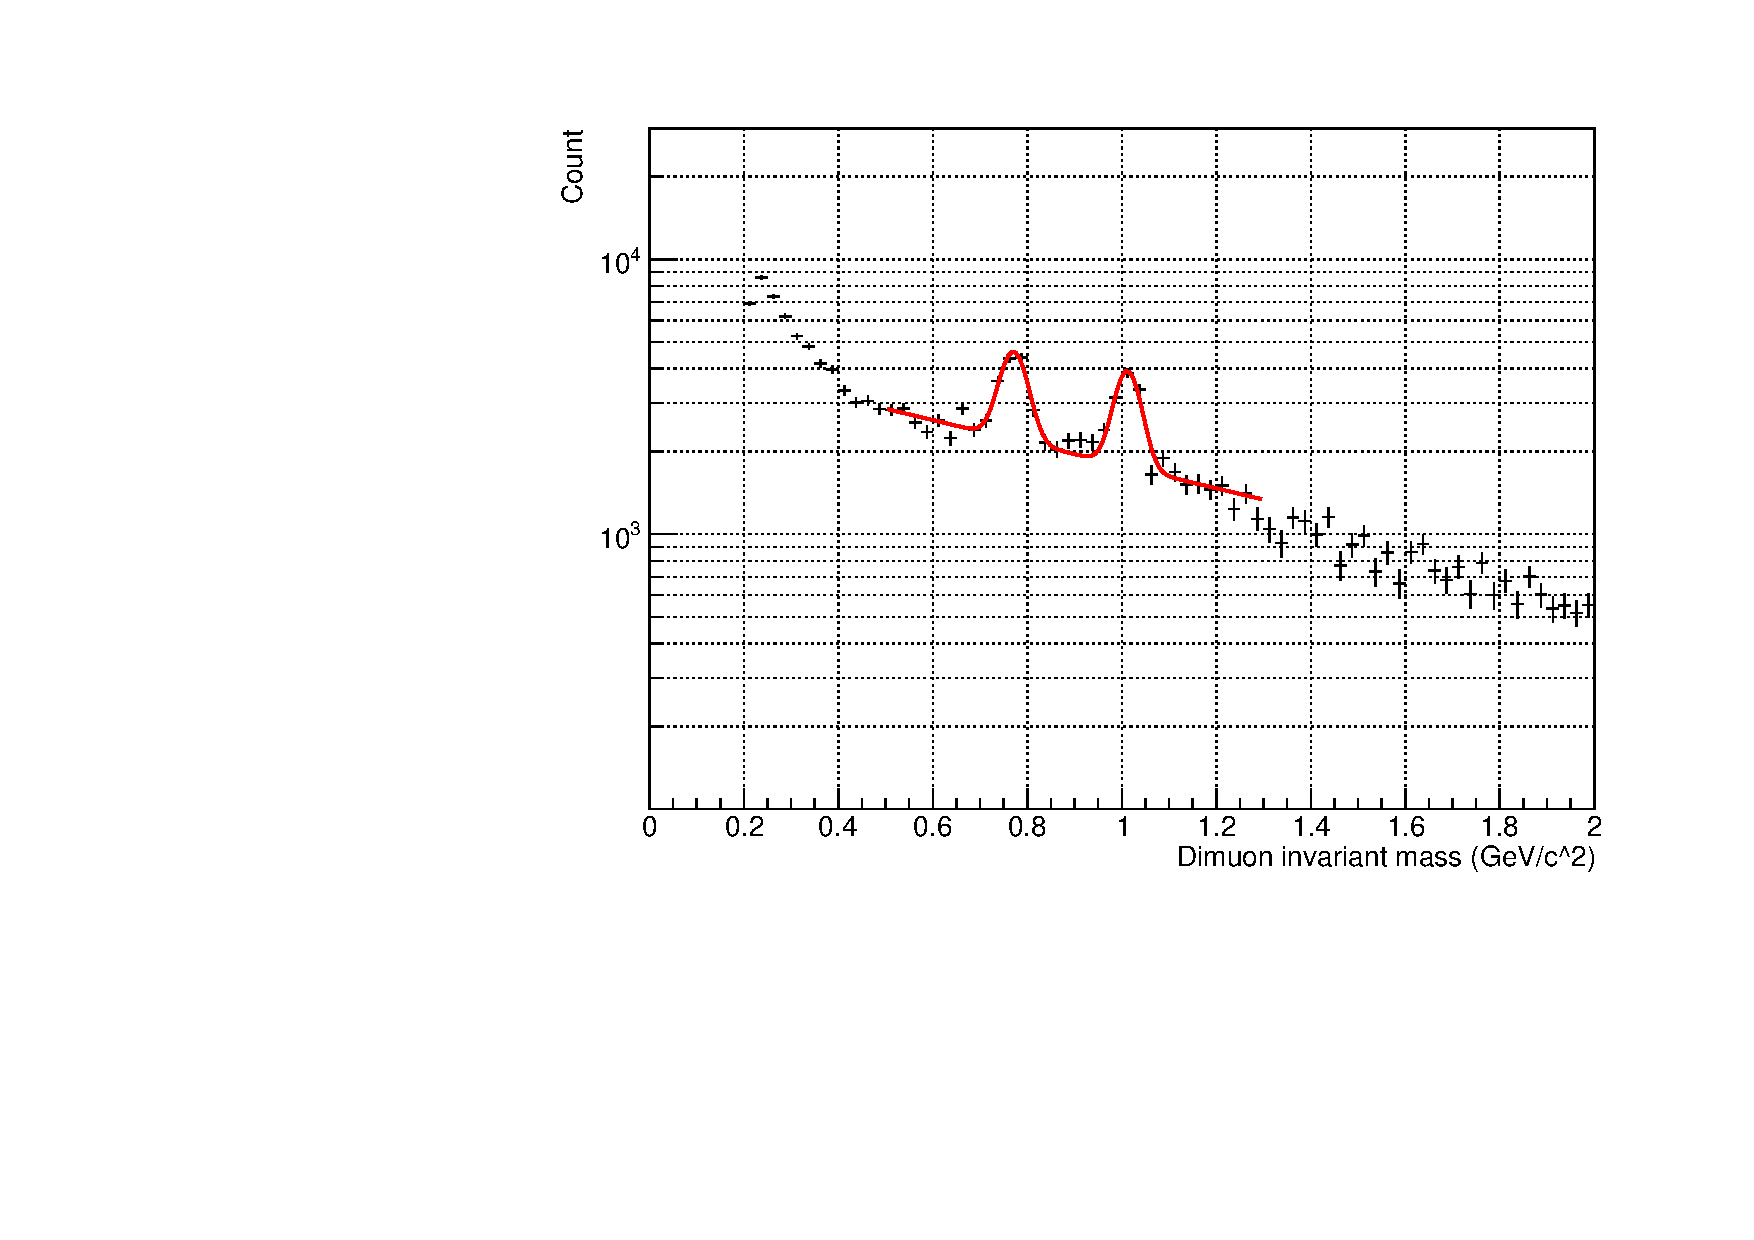
\includegraphics[width=\textwidth]{fig/3_4_4_Fit_chi2_200.pdf}
                    \caption*{MFT-MCH matching $\chi^2 < 200$}
                \end{minipage}
                \caption{MFT-MCH matching $\chi^2$カットを適用した際のピークフィットの結果}
                \label{Analysis:Dimuon:Matching_Fit}
            \end{figure}
            %need addition
            The horizontal axis represents the matching \(\chi^2\), while the vertical axis shows \(S/\sqrt{S+BG}\). As the cut value is reduced, the value of \(S/\sqrt{S+BG}\) increases. When a cut of \(\chi^2<30\) is applied, \(S/\sqrt{S+BG}\) reaches its maximum for both \(\omega\) and \(\phi\).\@ From this result, it is evident that the optimal matching \(\chi^2\) value is \(\chi^2<30\).\@
            \begin{figure}[htbp]
                \centering
                % Left figure
                \begin{minipage}{0.45\textwidth} % minipage for width specification
                    \centering
                    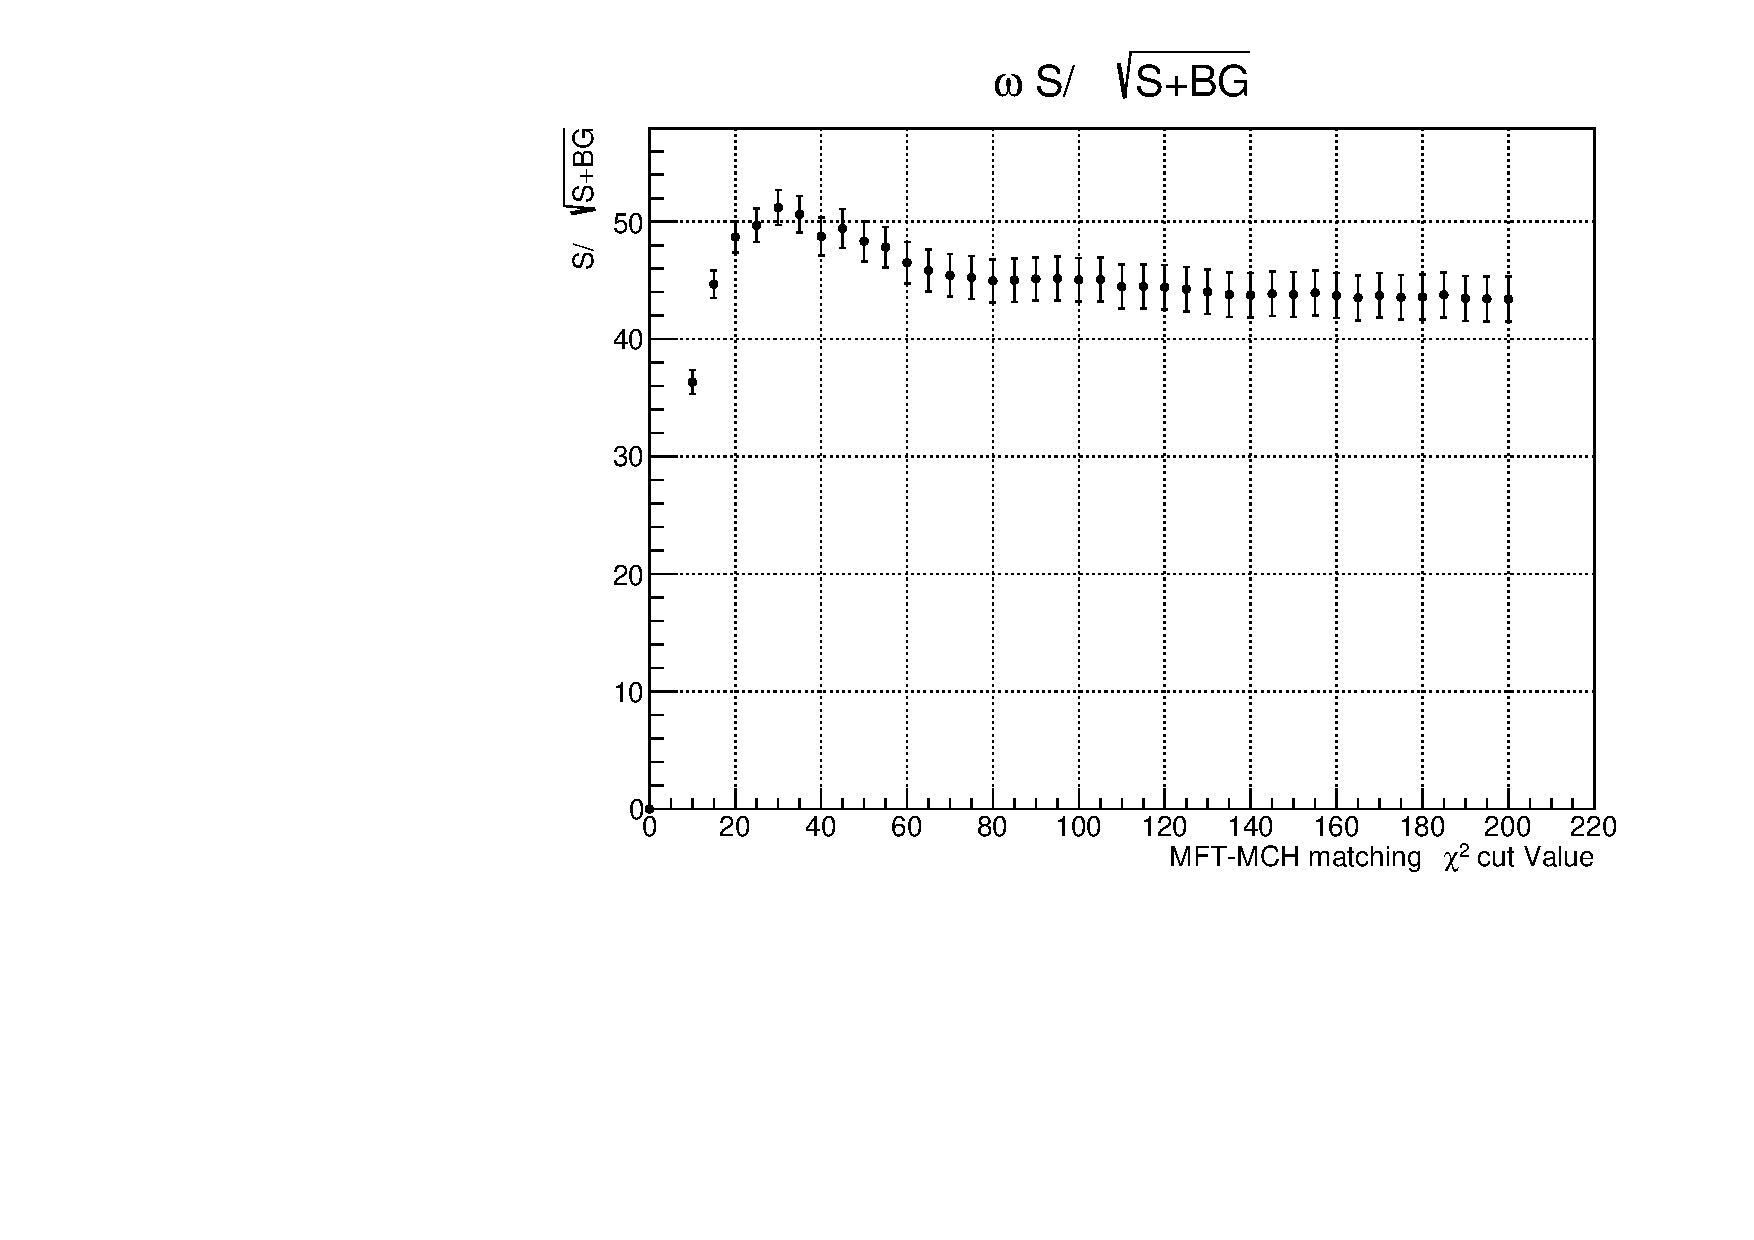
\includegraphics[width=\textwidth]{fig/3_4_4_omega_significance.pdf} % Left image
                    \caption{$\omega$ figure of merit}
                    \label{fig:omega_significance}
                \end{minipage}
                % Right figure
                \hfill
                \begin{minipage}{0.45\textwidth}
                    \centering
                    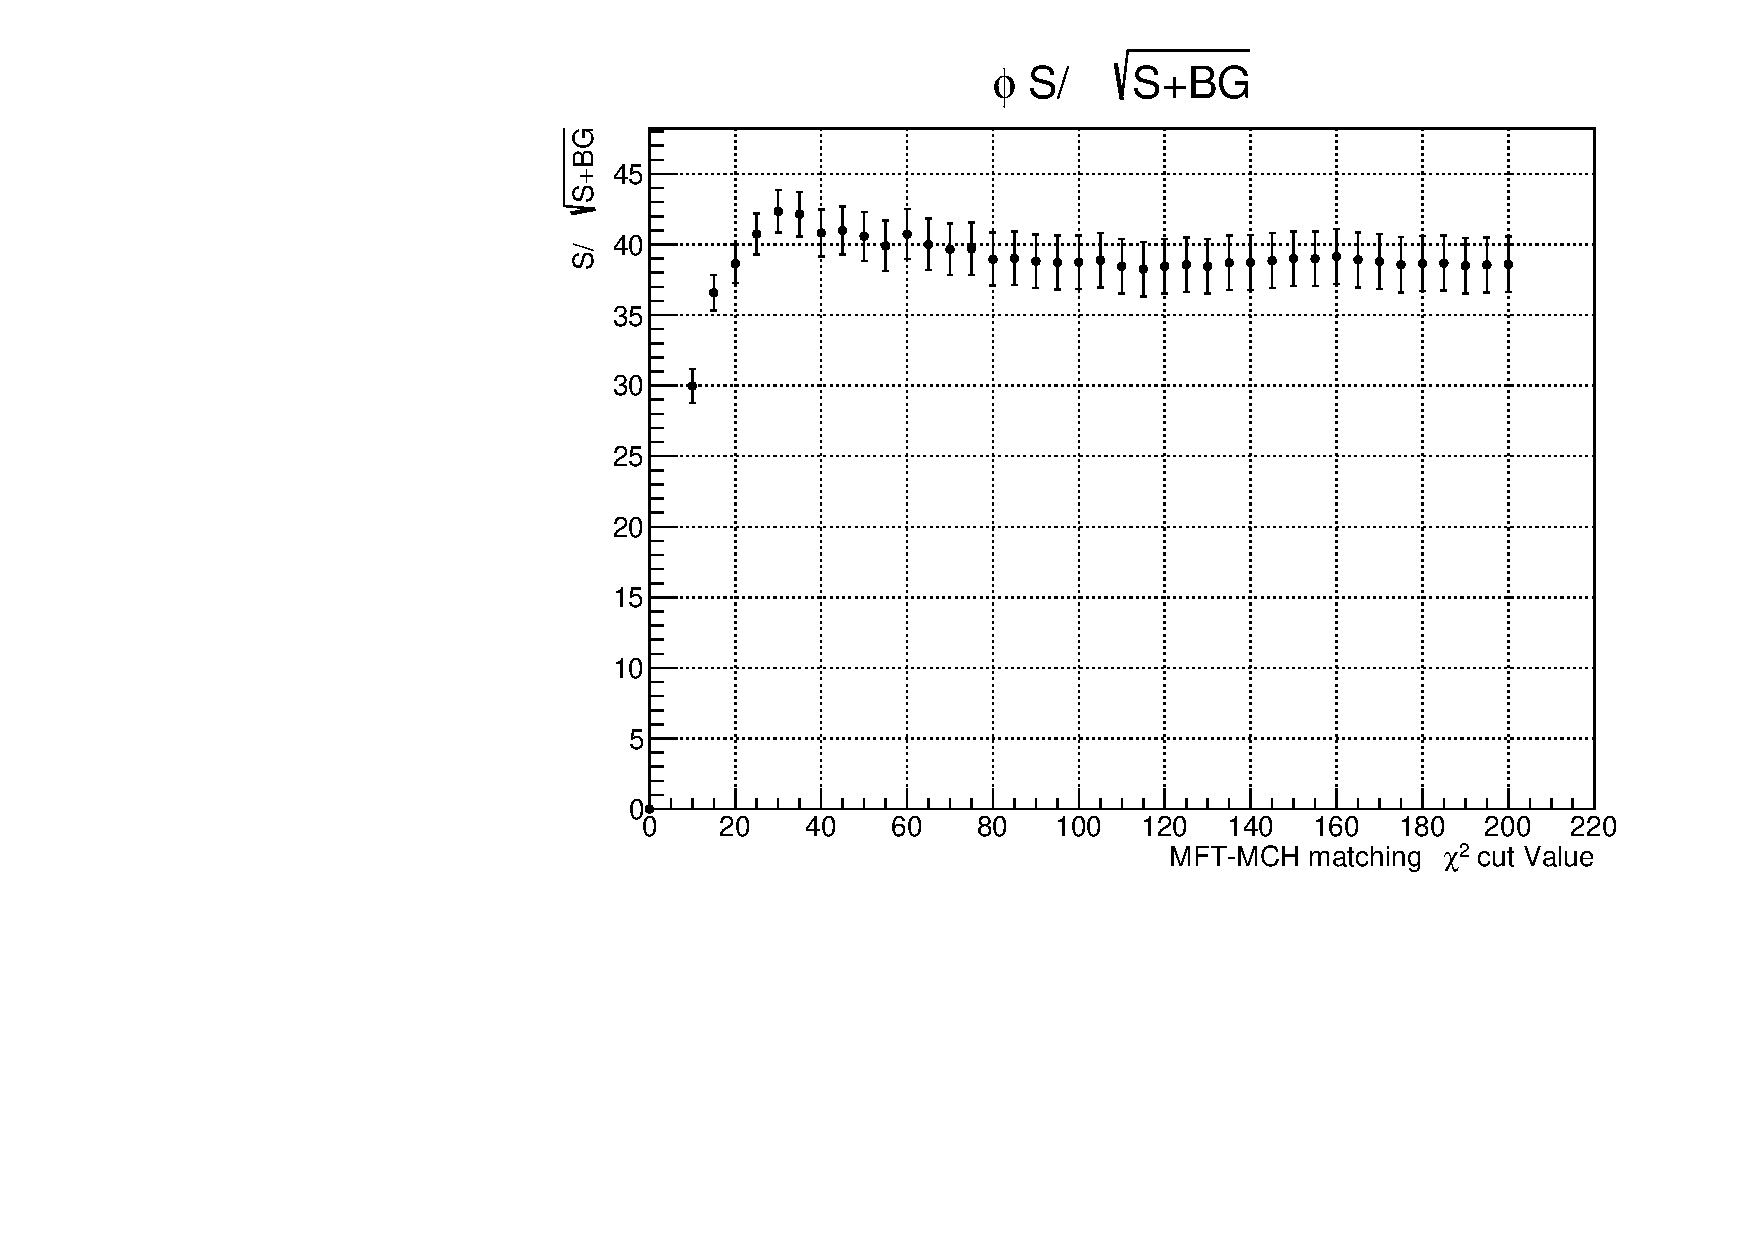
\includegraphics[width=\textwidth]{fig/3_4_4_phi_significance.pdf} % Right image
                    \caption{$\phi$ figure of merit}
                    \label{fig:phi_significance}
                \end{minipage}
            \end{figure}

        \subsubsection{Fake Match Track Removal Analysis of MFT-MCH-MID Track using MFT Track $\eta$ - MCH Track $\eta$}
        \label{Analysis:Matching}
            The \(\eta\) distribution of Global Tracks differs significantly from the true distribution. This discrepancy arises due to muon reconstruction involving the MFT, indicating issues with MFT-MCH matching. Fake matches contribute to this significantly distorted \(\eta\) distribution. By removing these distortions, it is shown that the resolution of \(\eta\), \(p_T\), and \(\phi\) for single muons improves. In this analysis, Fake matches are removed by utilising the difference in \(\eta\) between the MFT Track and MCH Track that constitute the Global Track. The dataset used is LHC24b1, which consists of Monte Carlo data of \(pp\) collisions at \(\sqrt{s} = 13.6\) TeV from minimum-bias events. This simulation data has been compared with real data, confirming that they exhibit the same behaviour. %\ref{Appendix:compair_Real_and_MC}
            \begin{figure}[H]
                \centering
                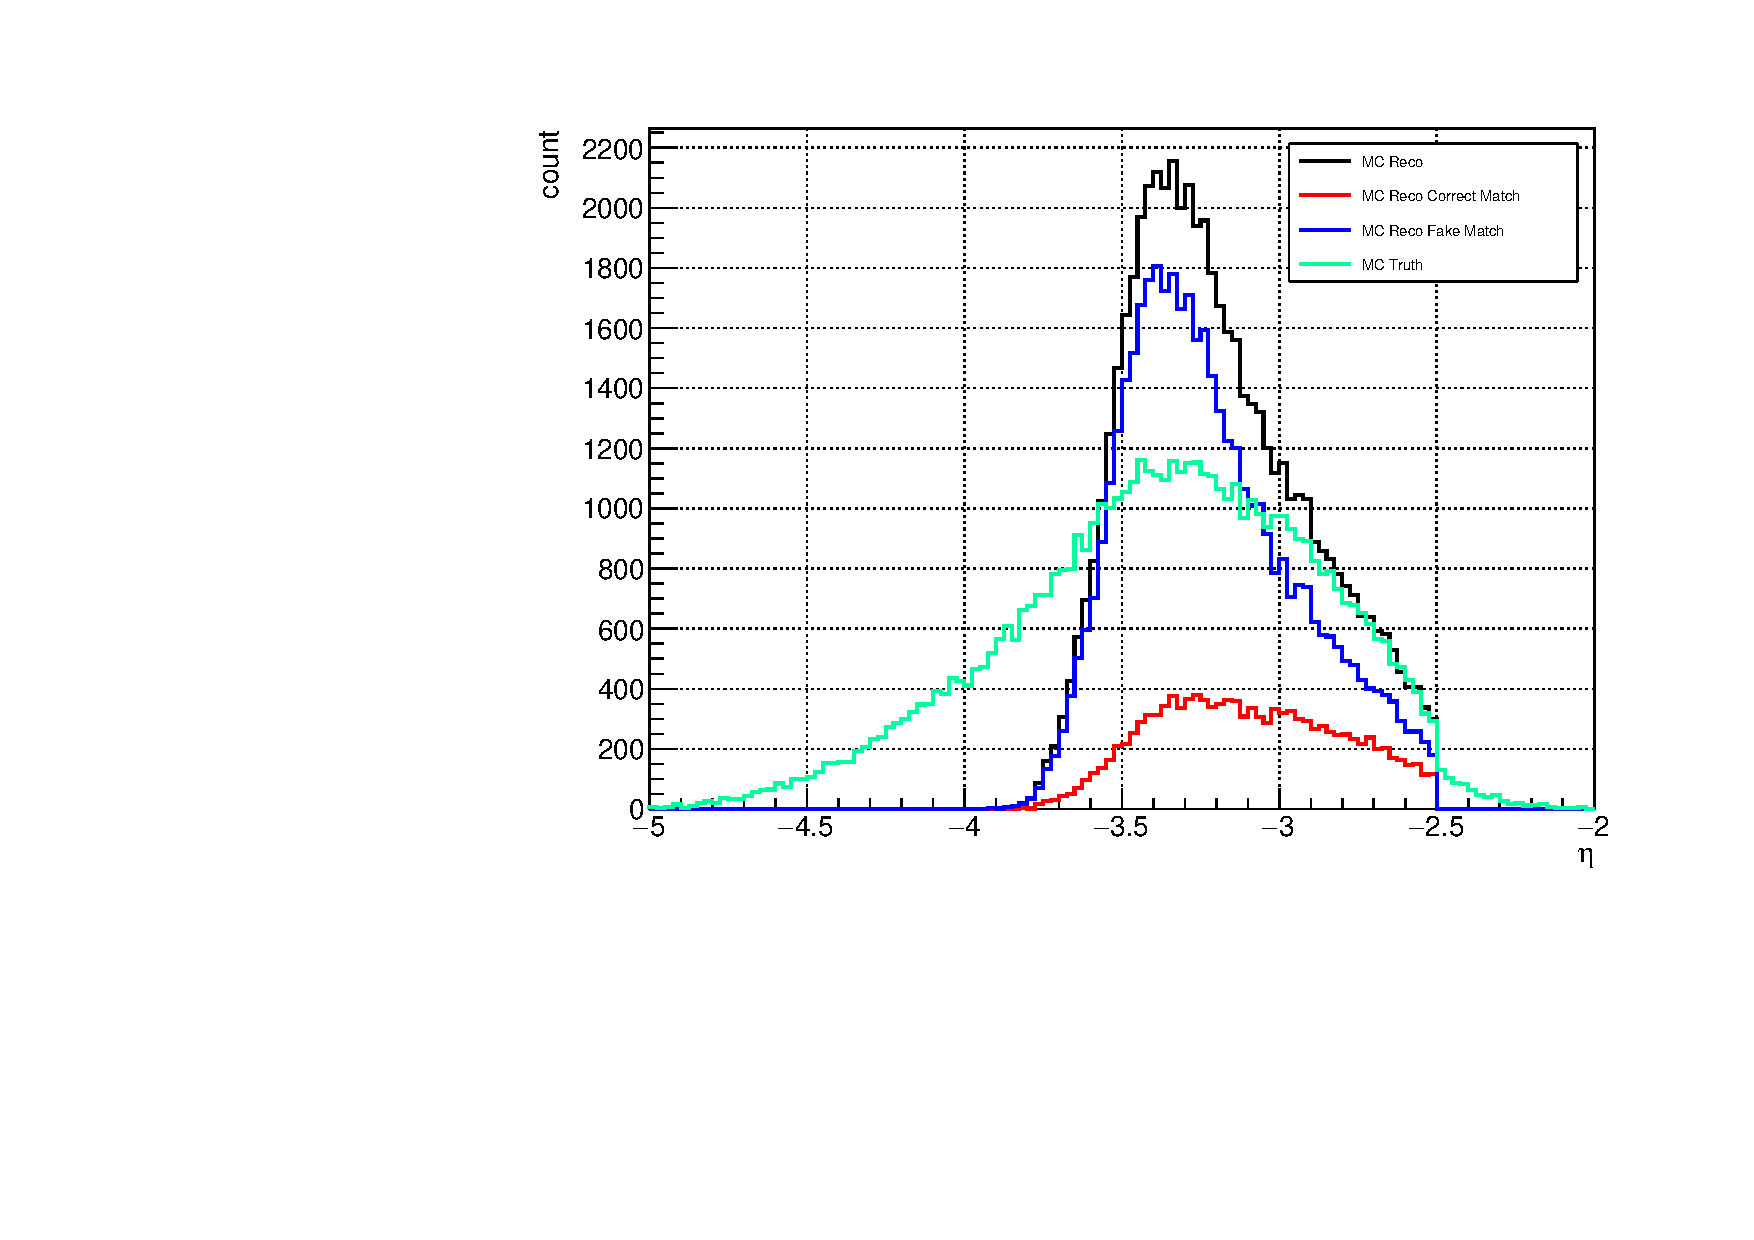
\includegraphics[keepaspectratio, scale=0.5]{fig/3_5_6_etacutno_eta.pdf}
                \caption{$\eta$ distribution of Global Track}
                \label{Analysis:Matching:eta}
            \end{figure}
            Figure \ref{Analysis:Matching:eta} shows the \(\eta\) distribution of Global Tracks for all \(p_T\) regions. The black histogram represents the reconstructed \(\eta\) distribution of Global Tracks. The blue histogram corresponds to the \(\eta\) distribution of reconstructed tracks identified as Fake matches, while the red histogram represents the \(\eta\) distribution of correctly matched tracks. The green histogram represents the true \(\eta\) distribution corresponding to the black reconstructed tracks.  
            Comparing the black reconstructed muon distribution with the green true distribution, the acceptance range of MFT-MCH-MID Tracks is \(-3.6 < \eta < -2.5\). However, in the green distribution, muons with \(\eta\) values smaller than \(-3.6\) are reconstructed within the \(-3.6 < \eta < -2.5\) range. This phenomenon is likely caused by muons that passed through the absorber and subsequently traversed the MCH-MID system while being outside the MFT acceptance. 
            To remove such tracks, a \(\Delta \eta\) cut is applied as (\ref{Deltaeta_eq}).
            \begin{eqnarray}
                \label{Deltaeta_eq}
                \Delta \eta = \text{MFT} \, \eta - \text{MCH} \, \eta  
            \end{eqnarray}
            For each track, \(\Delta \eta\) was calculated. Fig.\ref{Analysis:Matching:DeltaEta} shows the distribution. The black represents the distribution of reconstructed muons, the blue represents the distribution of Fake Match tracks, and the red represents the distribution of Correct Match tracks.
            \begin{figure}[H]
                \centering
                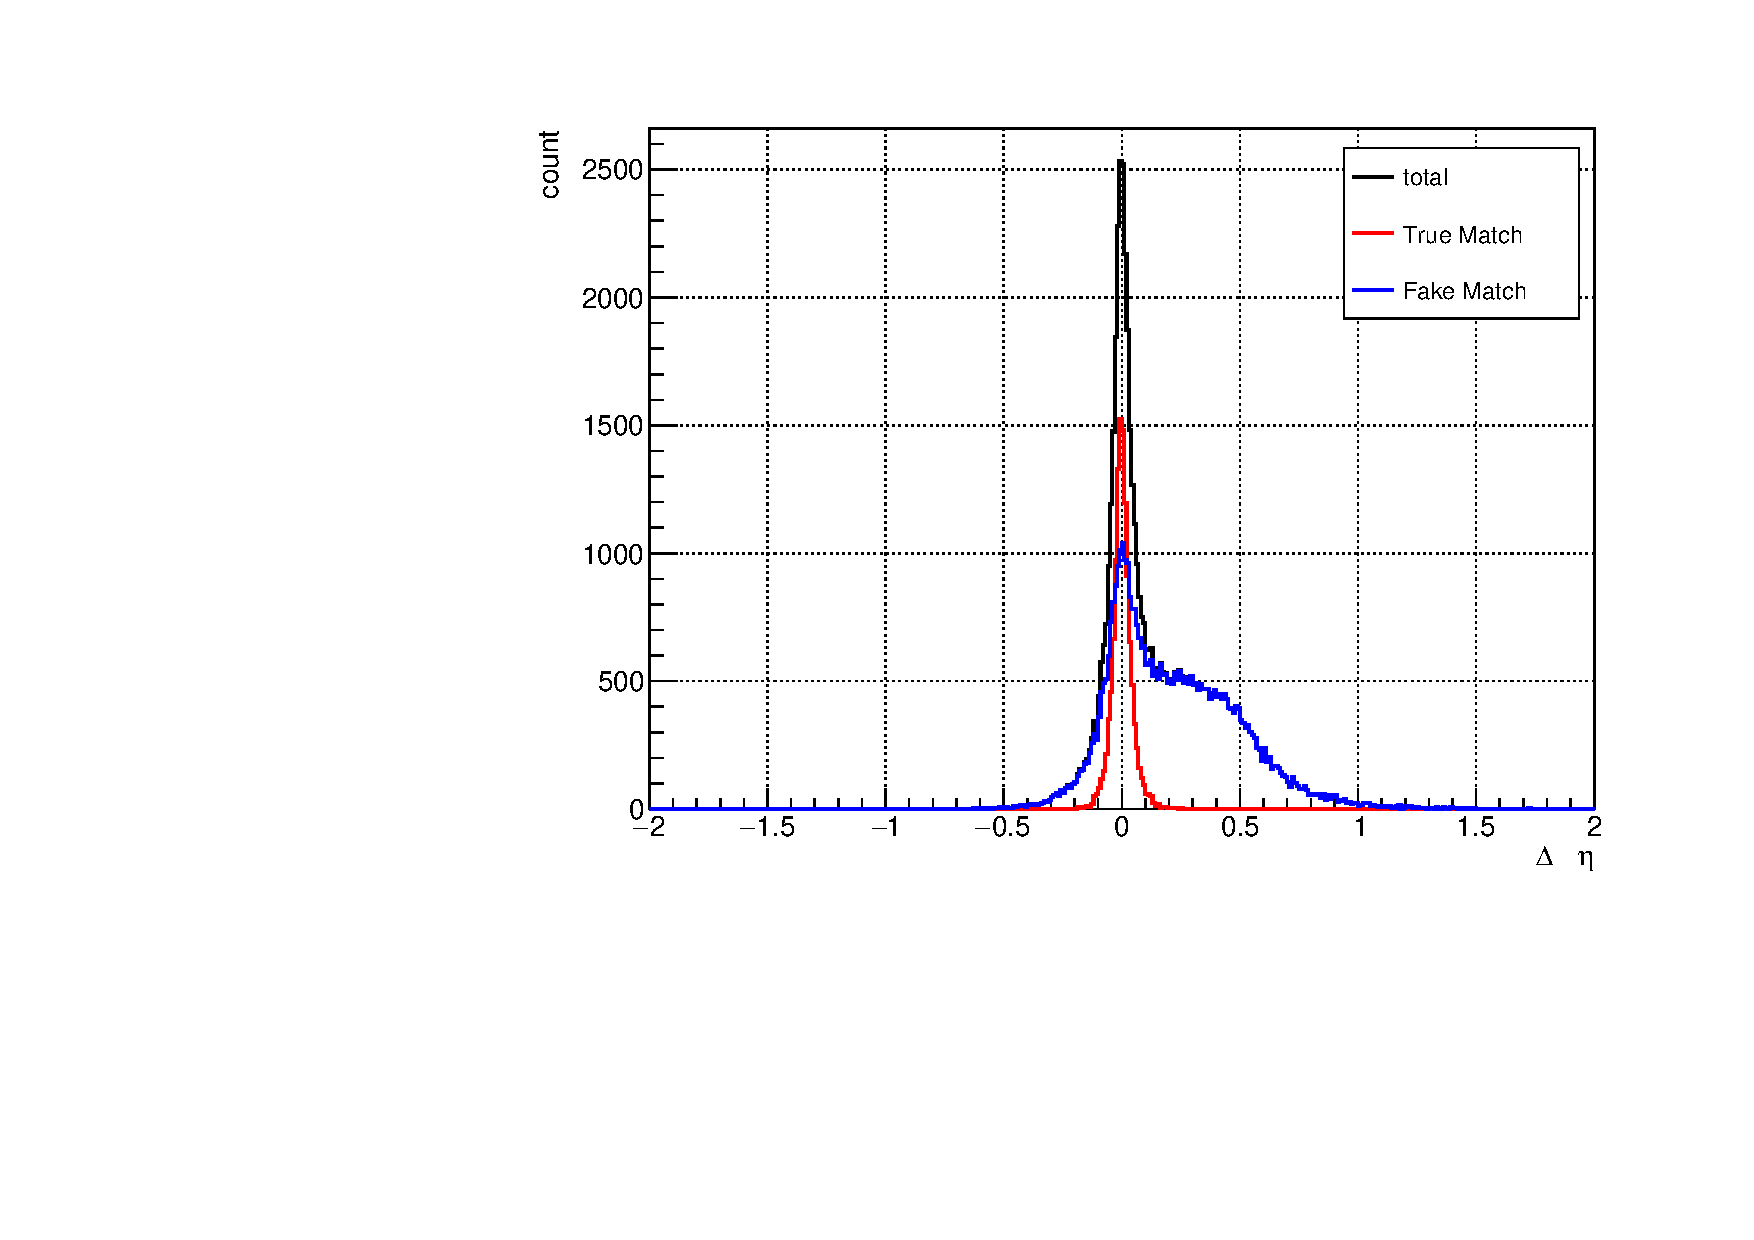
\includegraphics[keepaspectratio, scale=0.5]{fig/3_5_6_etacutno_deltaeta.pdf} % 右側の画像
                \caption{$\Delta \eta$ distribution}
                \label{Analysis:Matching:DeltaEta}
            \end{figure}
            For \( |\Delta \eta| > 0.2 \), Fake Match tracks dominate. The distributions and resolutions of each physical quantity are shown by applying a \( |\Delta \eta| < 0.2 \) cut to remove Fake Matches while retaining as many Correct Matches as possible.
            \begin{figure}[H]
                \centering
                % 左側の図
                \begin{minipage}{0.45\textwidth} % minipage で横幅を指定
                    \centering
                    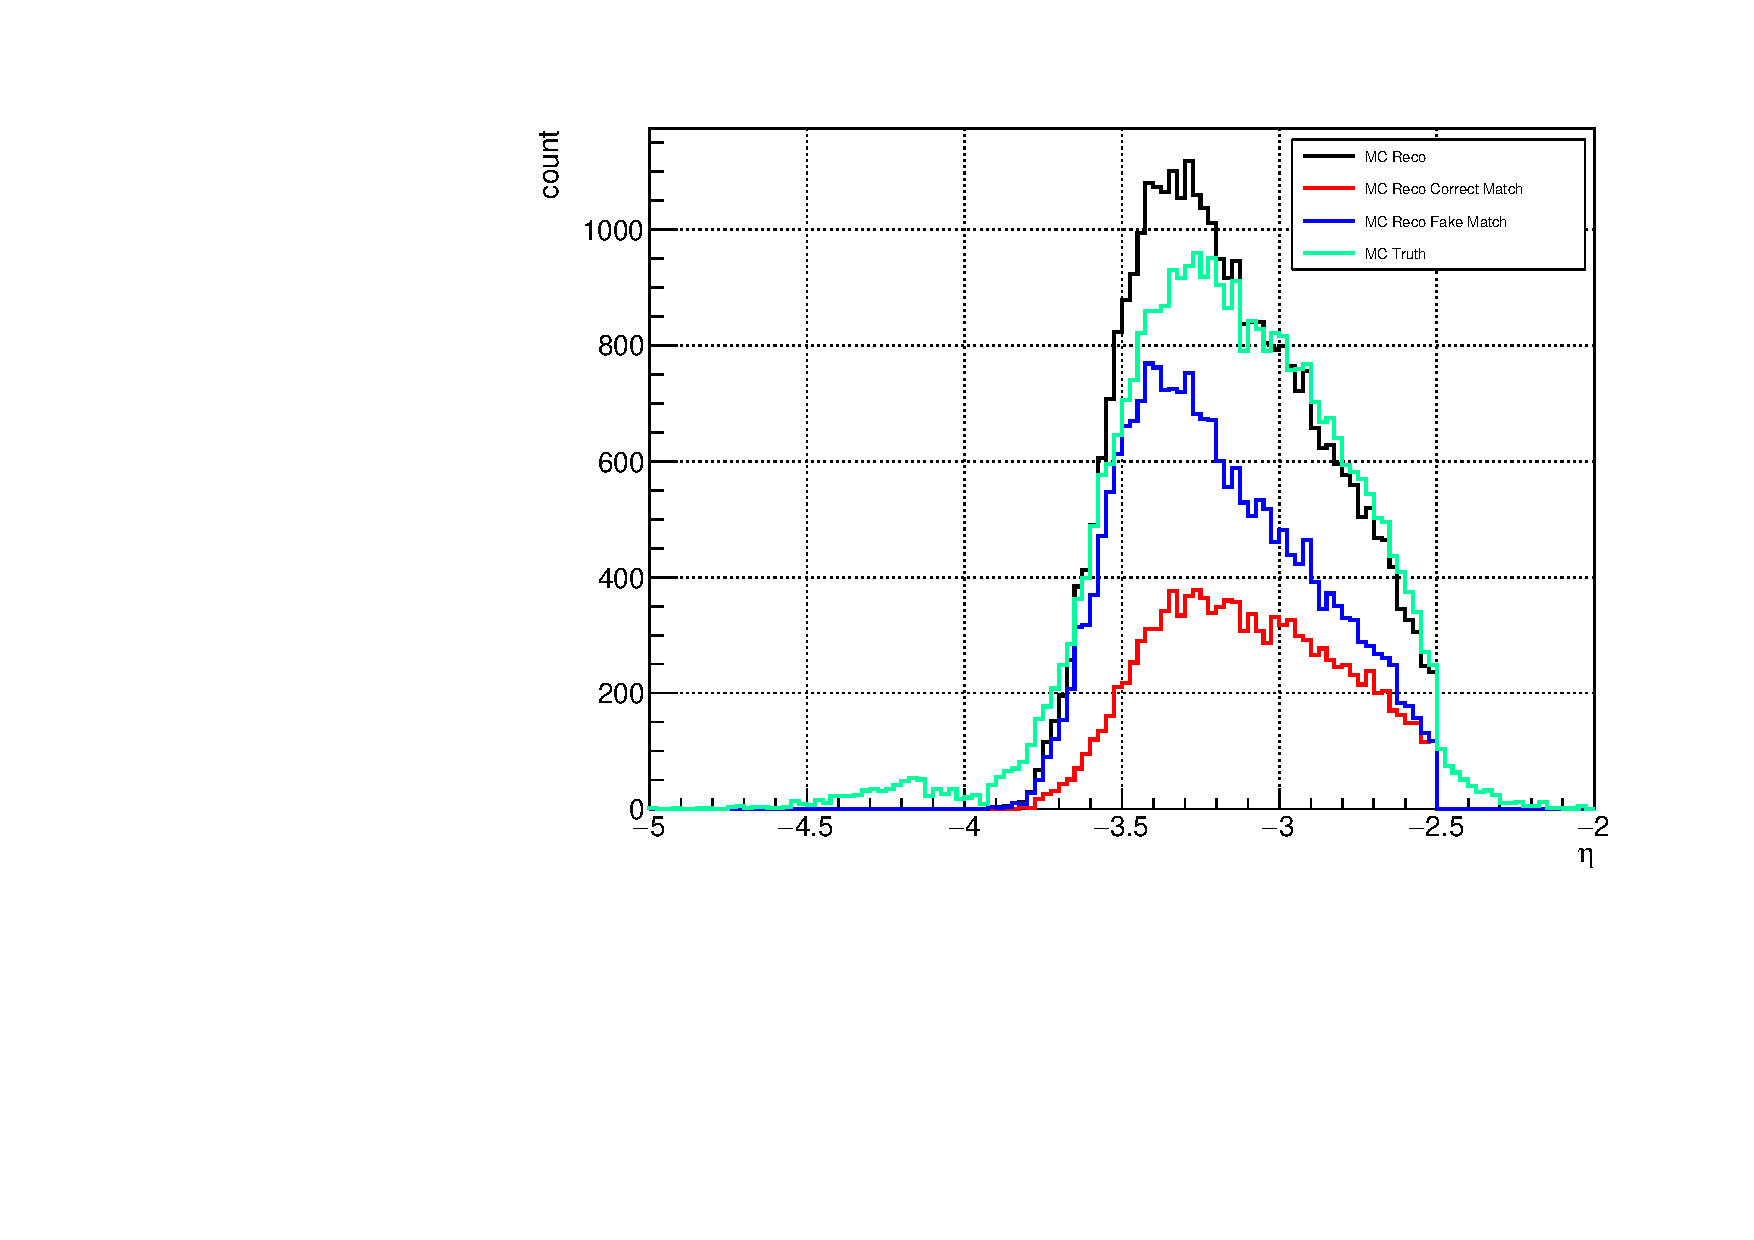
\includegraphics[width=\textwidth]{fig/3_5_6_etacut02_eta.pdf} % 左側の画像
                    \caption{The $\eta$ distribution of Global Tracks after the $\Delta \eta$ cut}
                    \label{Analysis:Matching:afterCut_eta}
                \end{minipage}
                % 右側の図
                \hfill
                \begin{minipage}{0.45\textwidth}
                    \centering
                    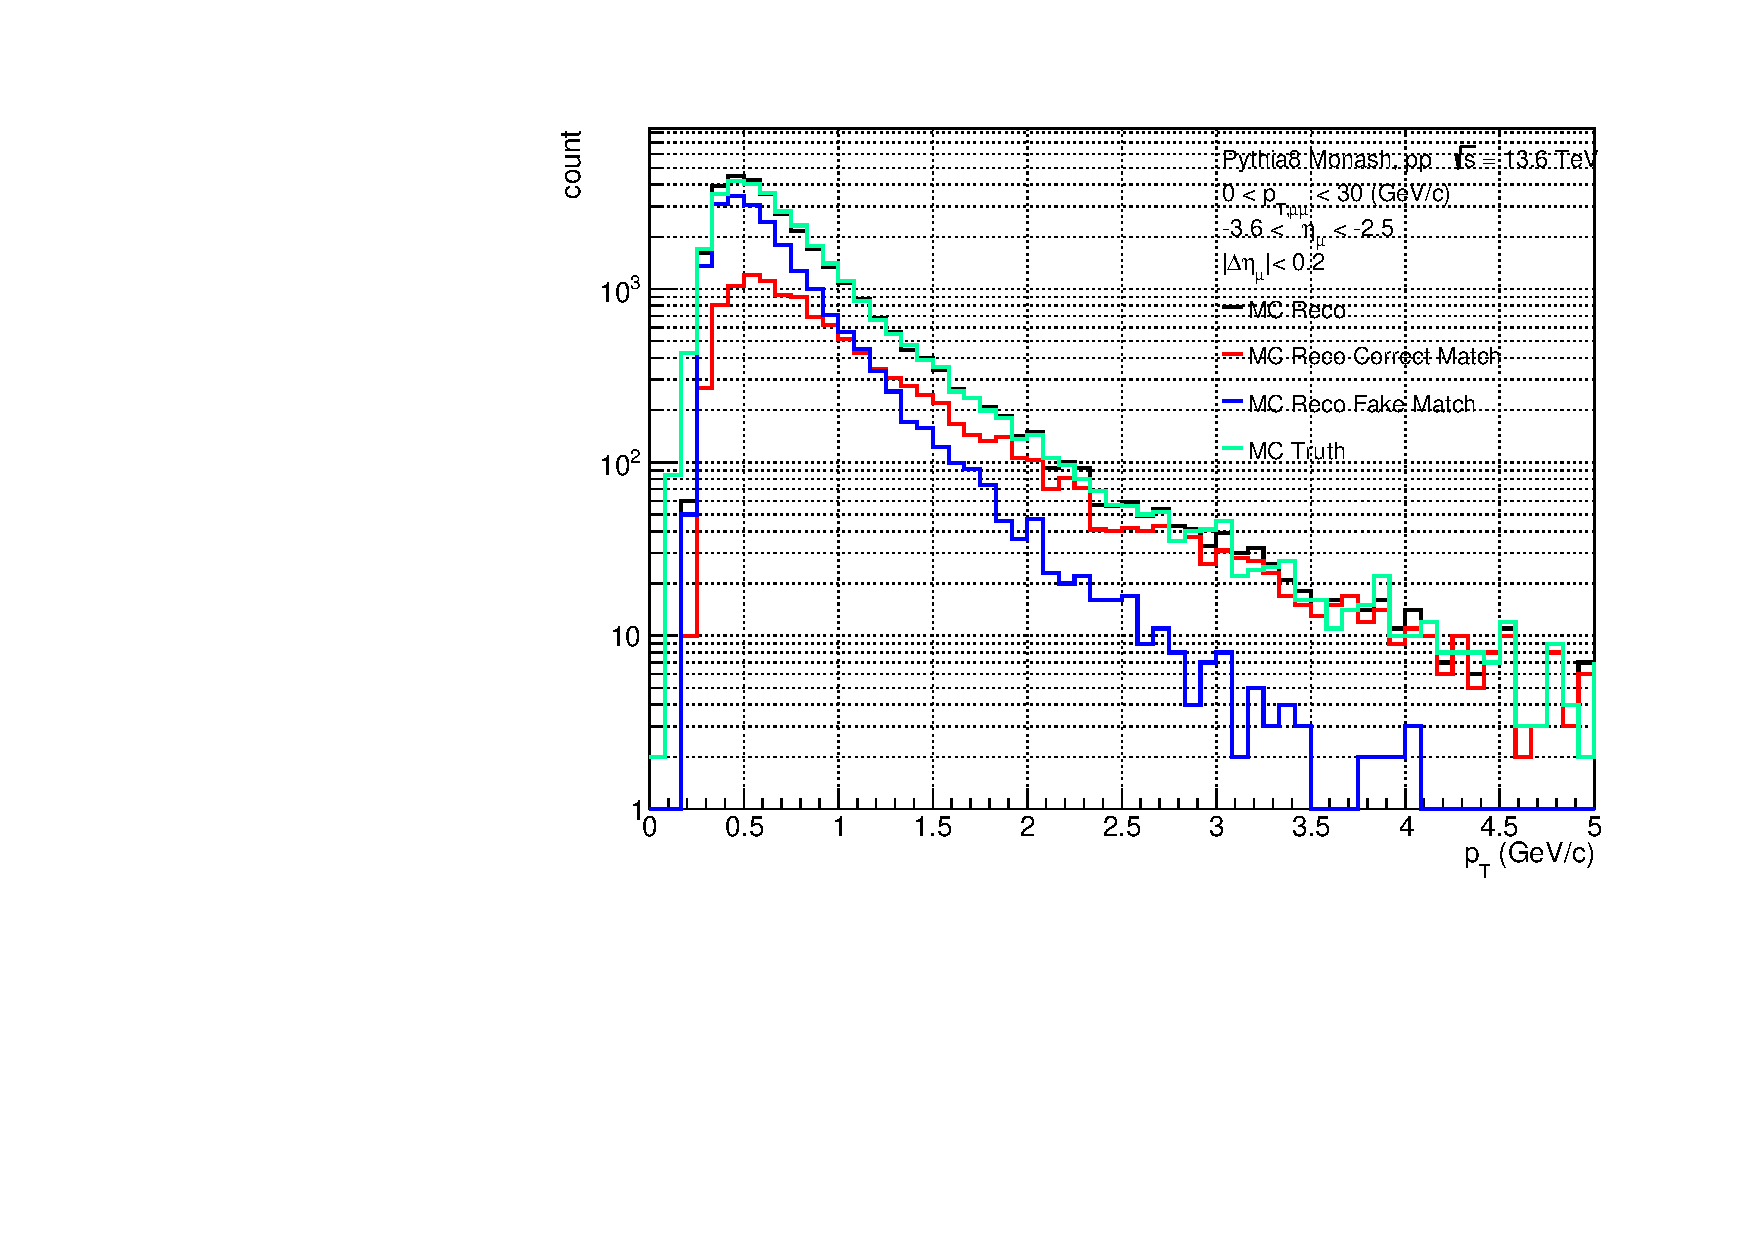
\includegraphics[width=\textwidth]{fig/3_5_6_etacut02_pt.pdf} % 右側の画像
                    \caption{The $p_T$ distribution of Global Tracks after the $\Delta \eta$ cut}
                    \label{Analysis:Matching:afterCut_pt}
                \end{minipage}-
            \end{figure}
            Figure \ref{Analysis:Matching:afterCut_eta} shows the \(\eta\) distribution after the \(\Delta \eta\) cut. Additionally, Figure \ref{Analysis:Matching:afterCut_pt} displays the \(p_T\) distribution after the \(\Delta \eta\) cut. As in Figure \ref{Analysis:Matching:eta}, the black histogram represents all reconstructed muon tracks, the red represents Correct match tracks, and the blue represents Fake Match tracks. The green histogram corresponds to the true \(\eta\) distribution for the black muons. Comparing the green distribution of \(\eta\) after the cut with Figure \ref{Analysis:Matching:eta}, we see that the muons distributed at \(\eta < -3.8\) have been removed. Furthermore, this cut removes many Fake match tracks in the range of \(-3.6 < \eta < -3.2\). However, as seen from Figure \ref{Analysis:Matching:afterCut_pt}, Fake matches originating from low transverse momentum remain.
            \begin{figure}[H]
                \centering
                    \begin{minipage}{0.45\textwidth}
                        \centering
                        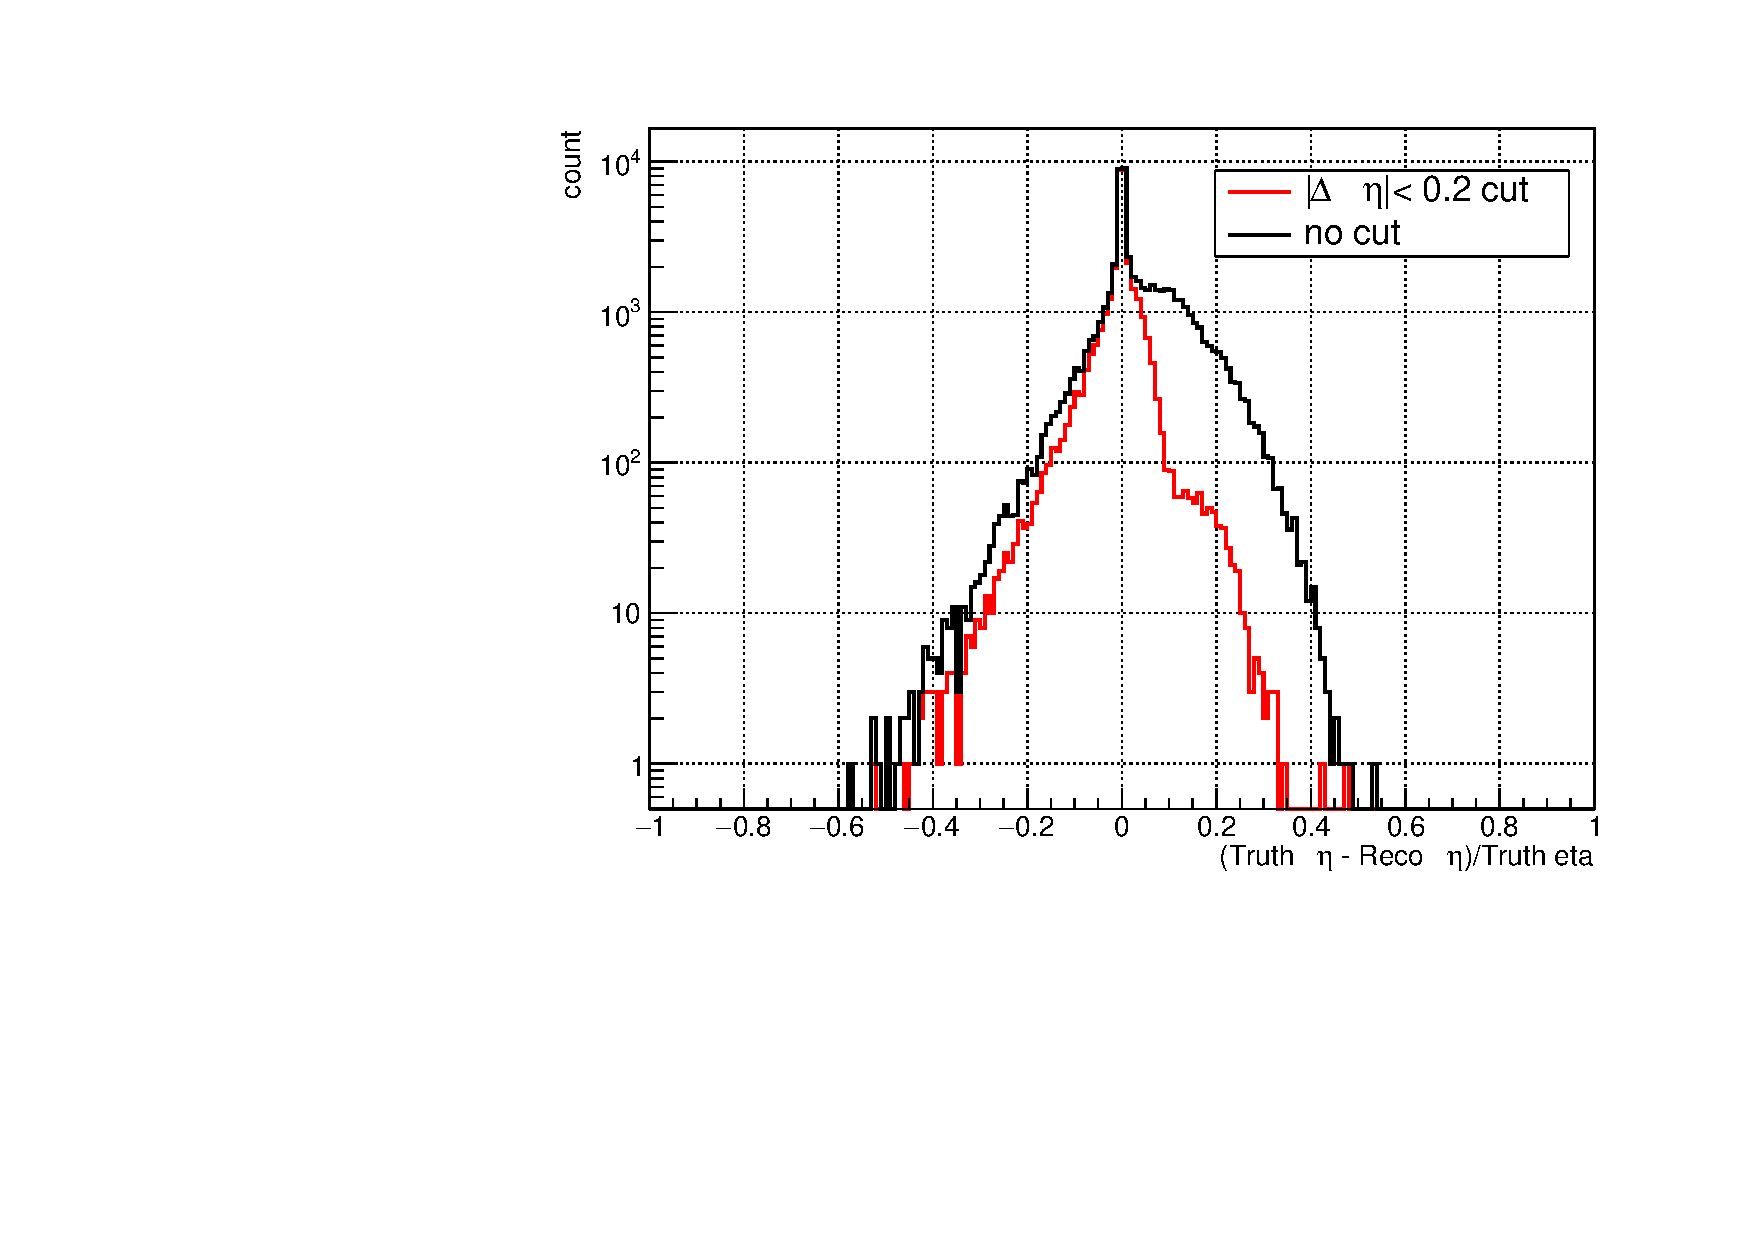
\includegraphics[width=\textwidth]{fig/3_5_6_reso_eta.pdf} 
                        \caption{Resolution of $\eta$}
                        \label{Analysis:Matching:pt resolution}
                    \end{minipage}
                    \begin{minipage}{0.45\textwidth}
                        \centering
                        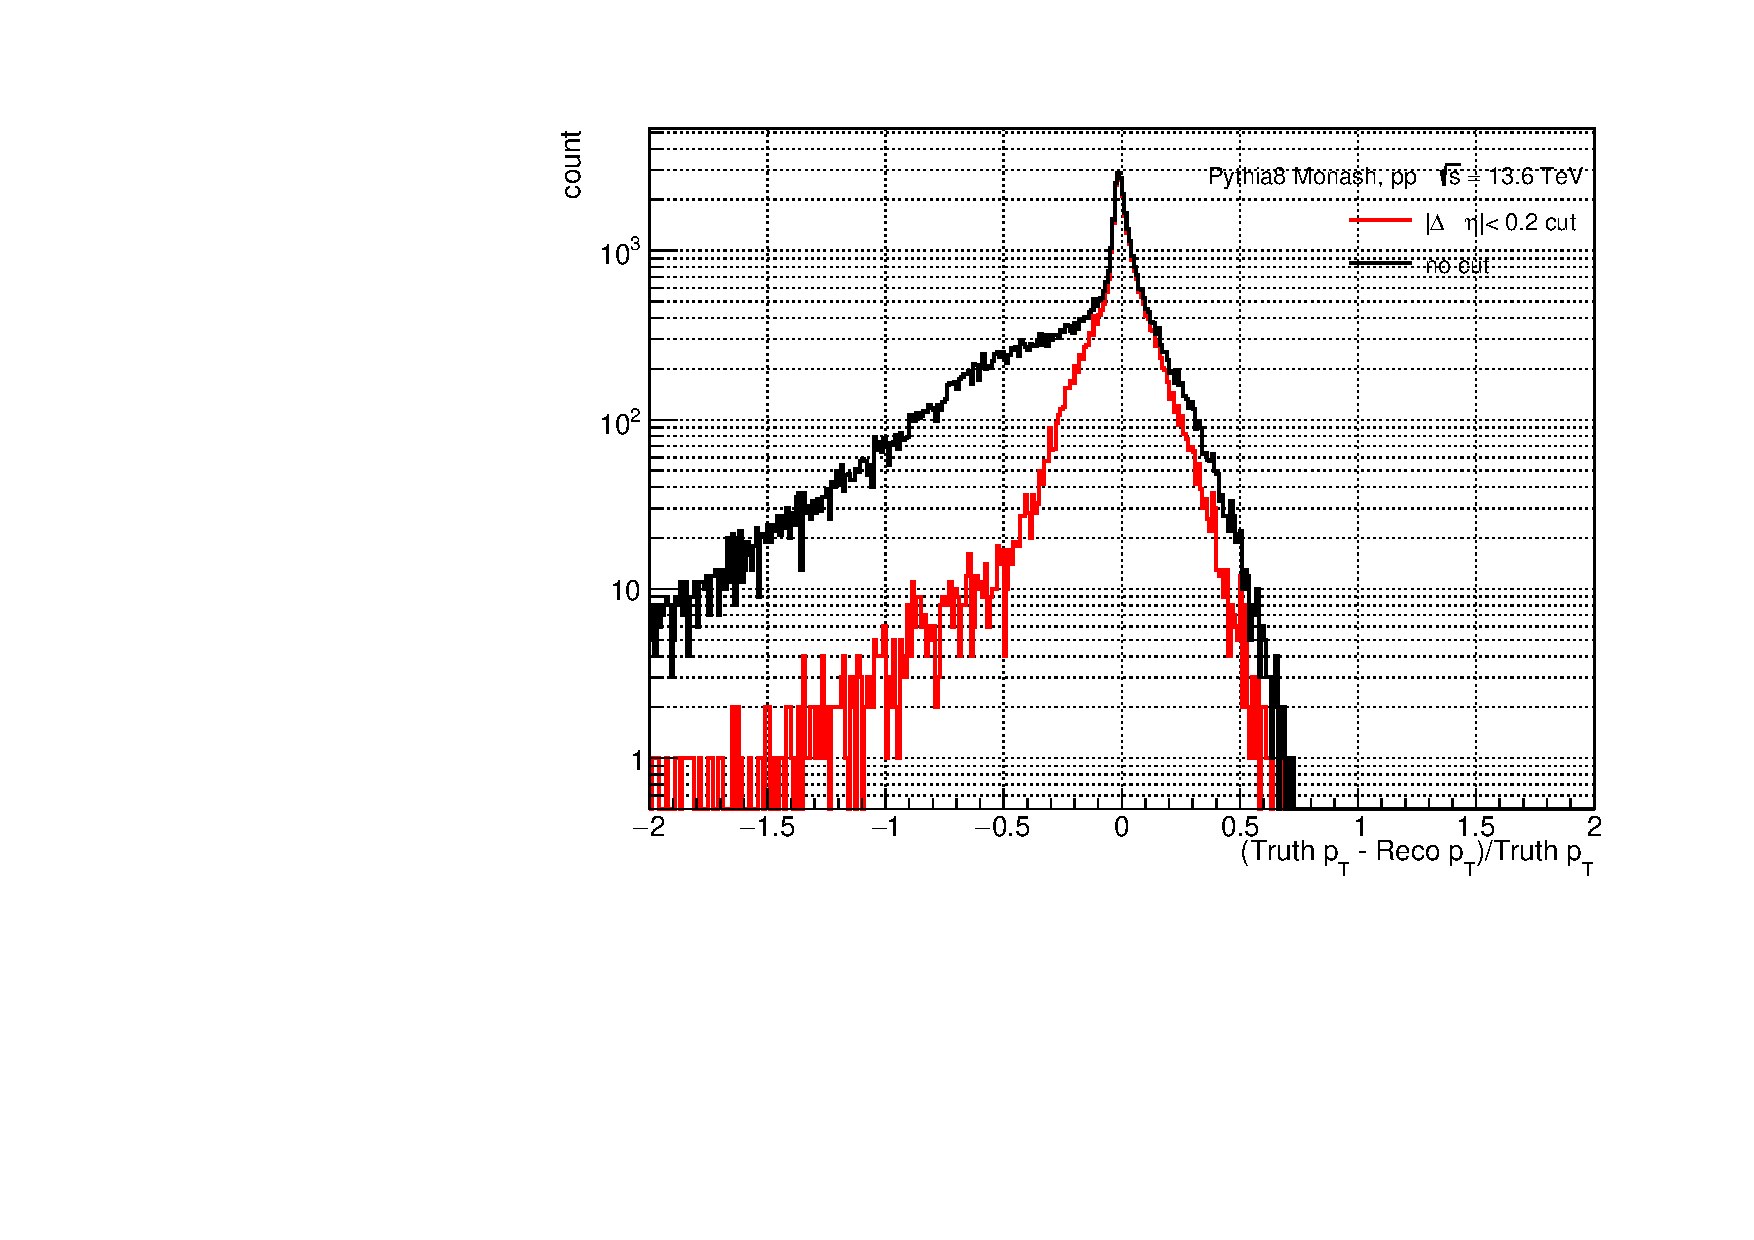
\includegraphics[width=\textwidth]{fig/3_5_6_reso_pt.pdf} 
                        \caption{Resolution of $p_T$}
                        \label{Analysis:Matching:eta resolution}
                    \end{minipage}
                \end{figure}
                \begin{figure}[H]
                    \centering
                    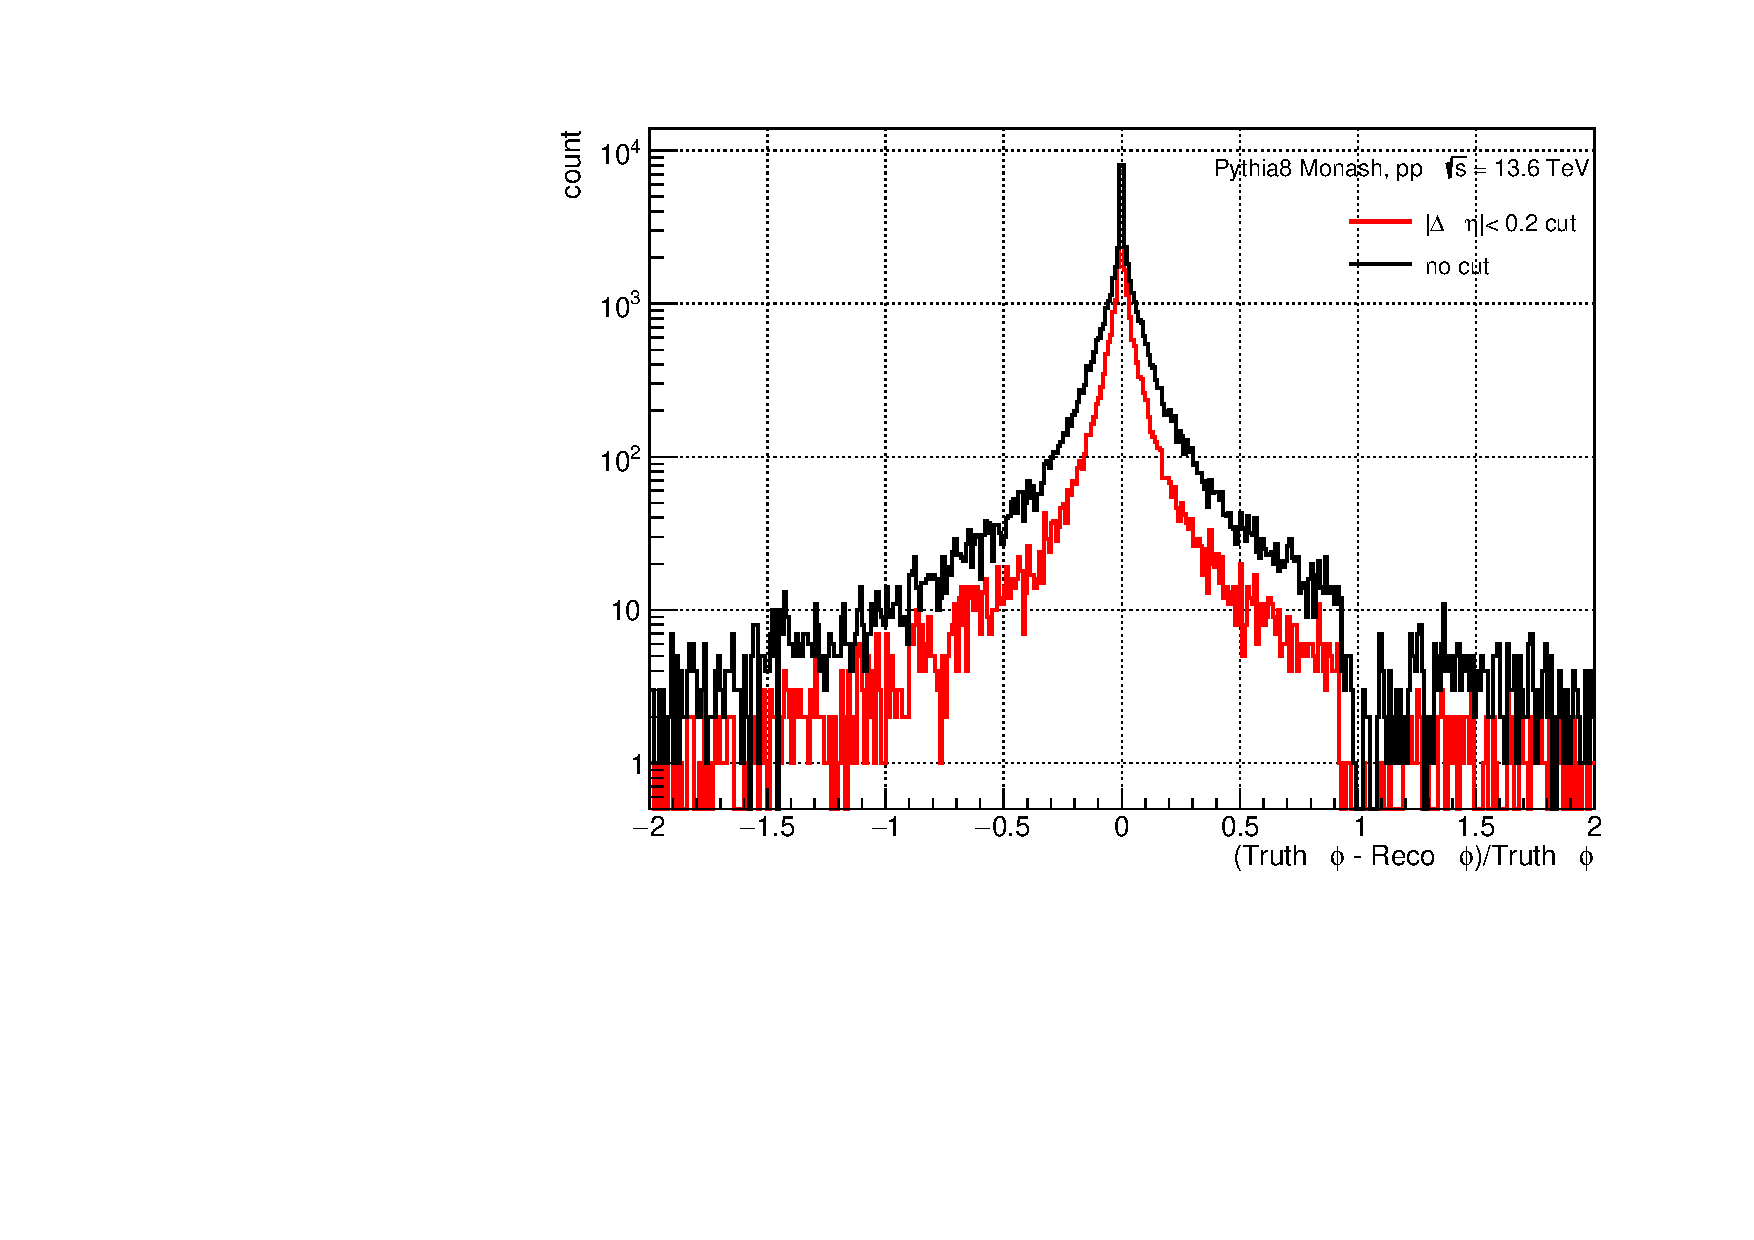
\includegraphics[keepaspectratio, scale=0.4]{fig/3_5_6_reso_phi.pdf} 
                    \caption{Resolution of $\phi$}
                    \label{Analysis:Matching:phi resolution}
                \end{figure}
                Figures \ref{Analysis:Matching:pt resolution}, \ref{Analysis:Matching:eta resolution}, and \ref{Analysis:Matching:phi resolution} show the resolution of \(p_T\), \(\eta\), and \(\phi\), respectively. The horizontal axis represents the resolution, calculated by subtracting the reconstructed quantity from the true physical quantity and dividing it by the true value. The vertical axis represents the count. The black distribution shows the resolution without applying the \(\Delta \eta\) cut, while the red distribution shows the tracks after applying the \(|\Delta \eta| < 0.2\) cut. By comparing the black and red histograms, it is clear that the resolution has a small value for all distributions. This shows that the resolution improves with the cut. Next, we will describe the efficiency and matching purity improvements due to the cut.
            \begin{figure}[htbp]
                \centering
                \begin{minipage}{0.45\textwidth}
                    \centering
                    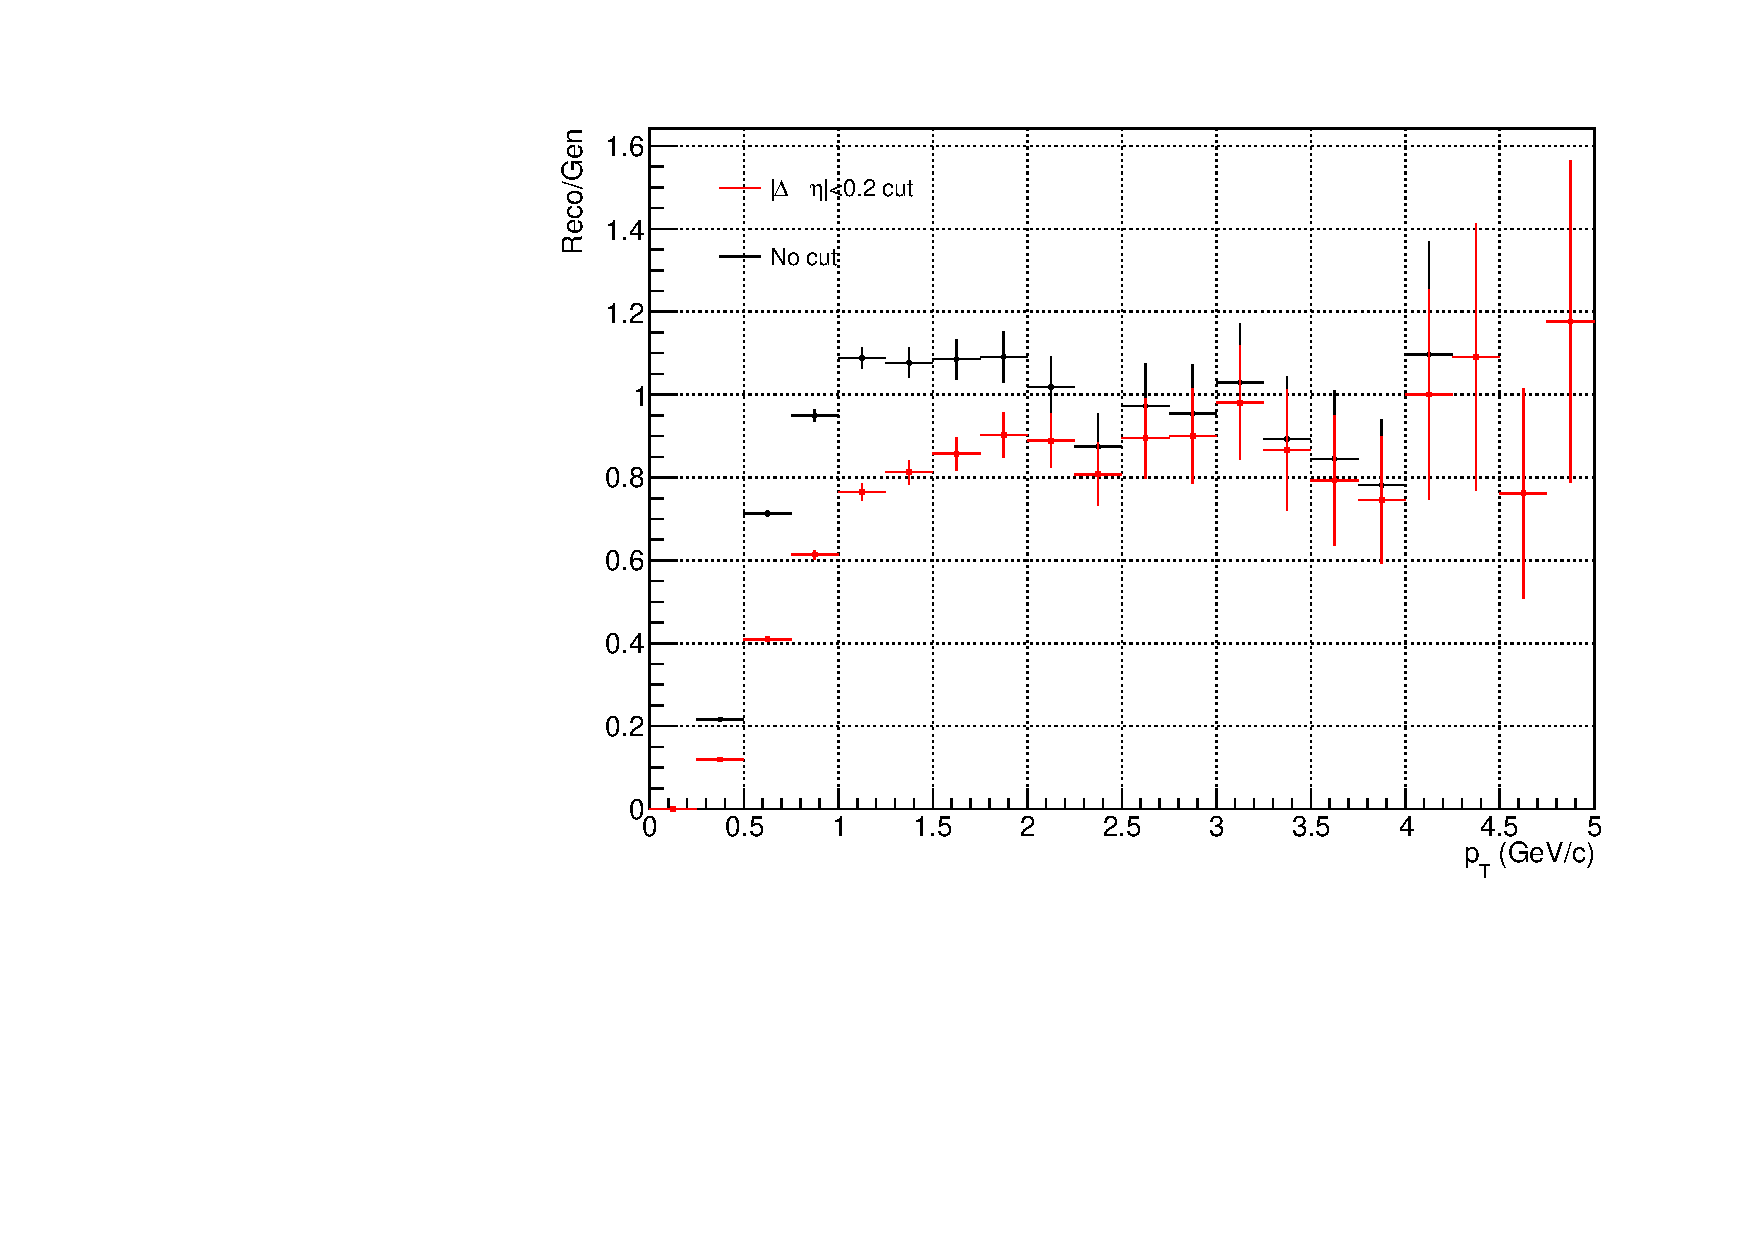
\includegraphics[width=\textwidth]{fig/3_5_6_efficiency_pt.pdf}
                    \caption{Efficency of $p_T$}
                    \label{Efficency_of_pt}
                \end{minipage}
                \hfill
                \begin{minipage}{0.45\textwidth}
                \centering
                    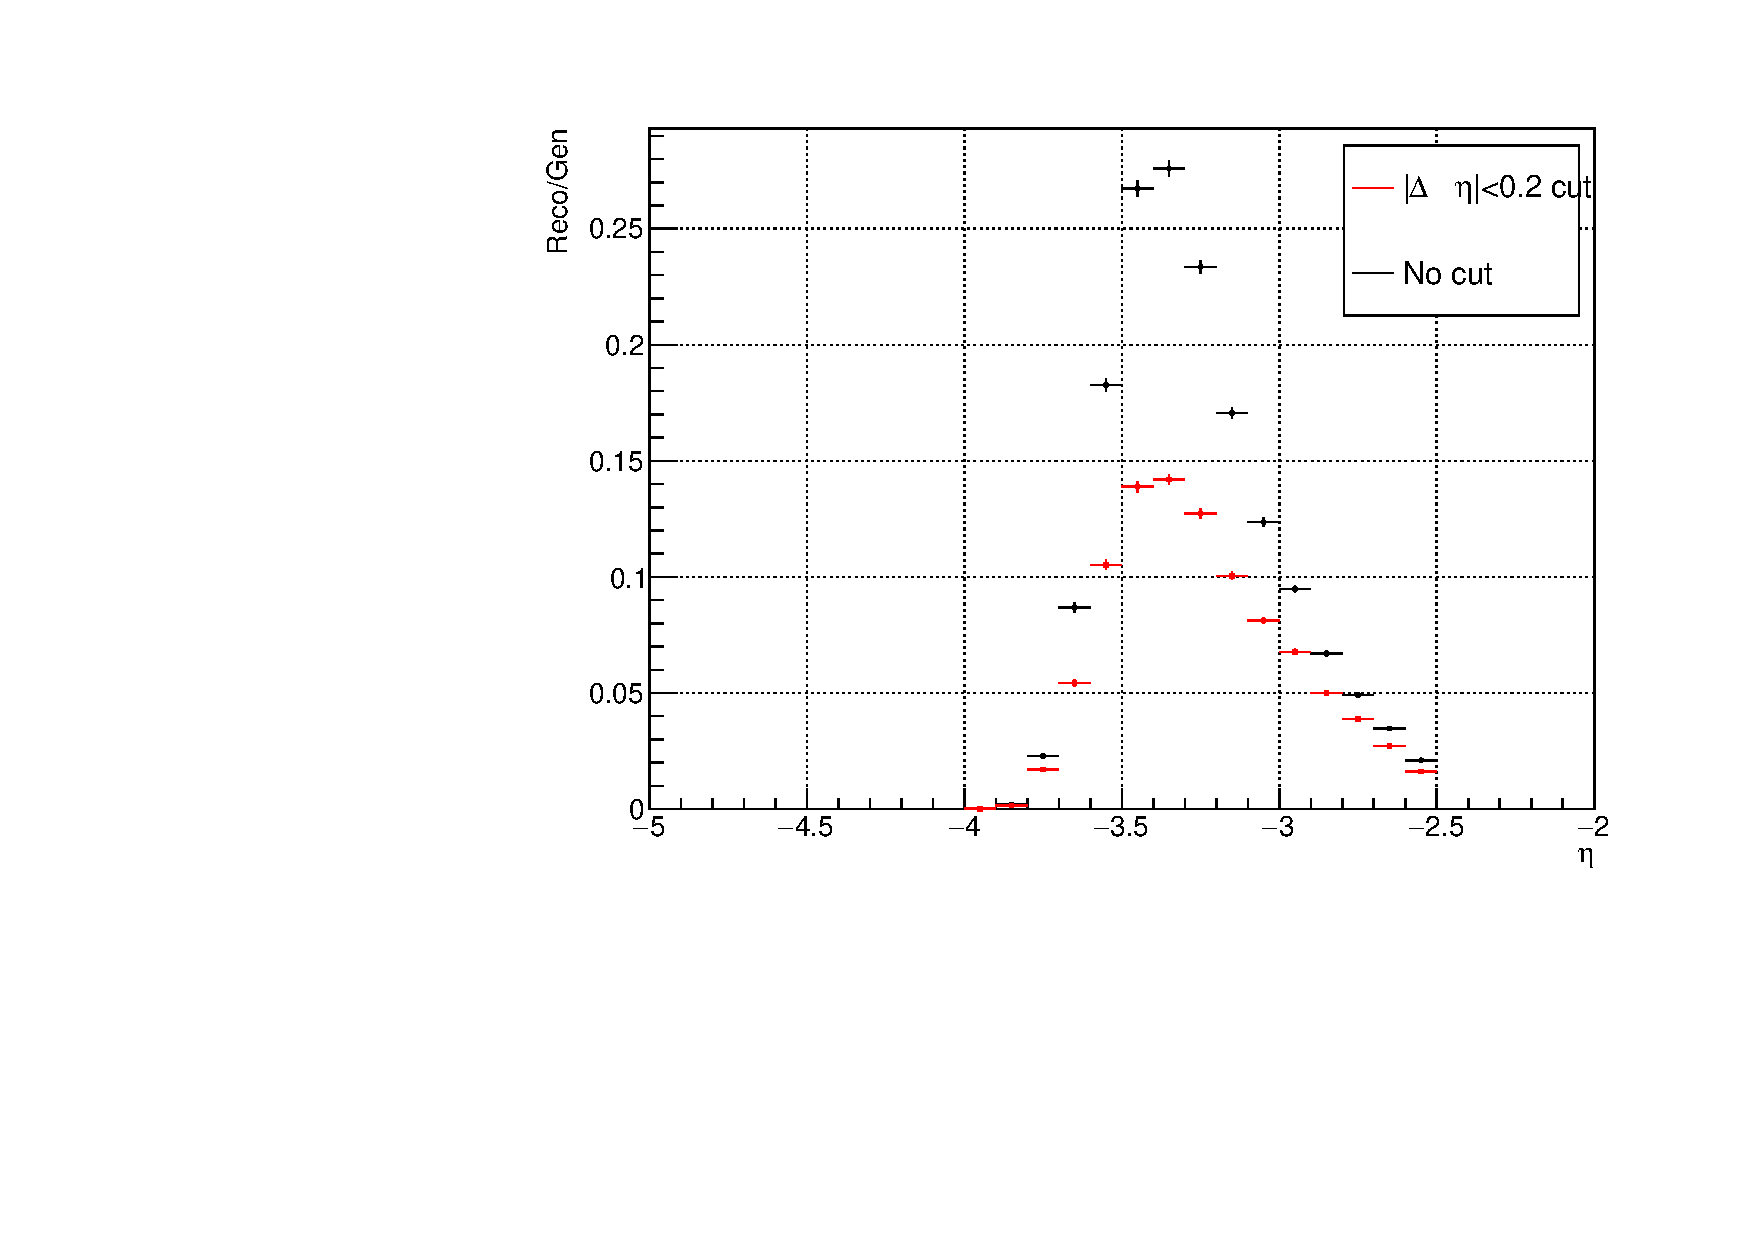
\includegraphics[width=\textwidth]{fig/3_5_6_efficiency_eta.pdf}
                    \caption{Efficency of $\eta$}
                    \label{Efficency_of_eta}
                \end{minipage}
                \\
                \vspace{1em}
                \begin{minipage}{0.45\textwidth}
                \centering
                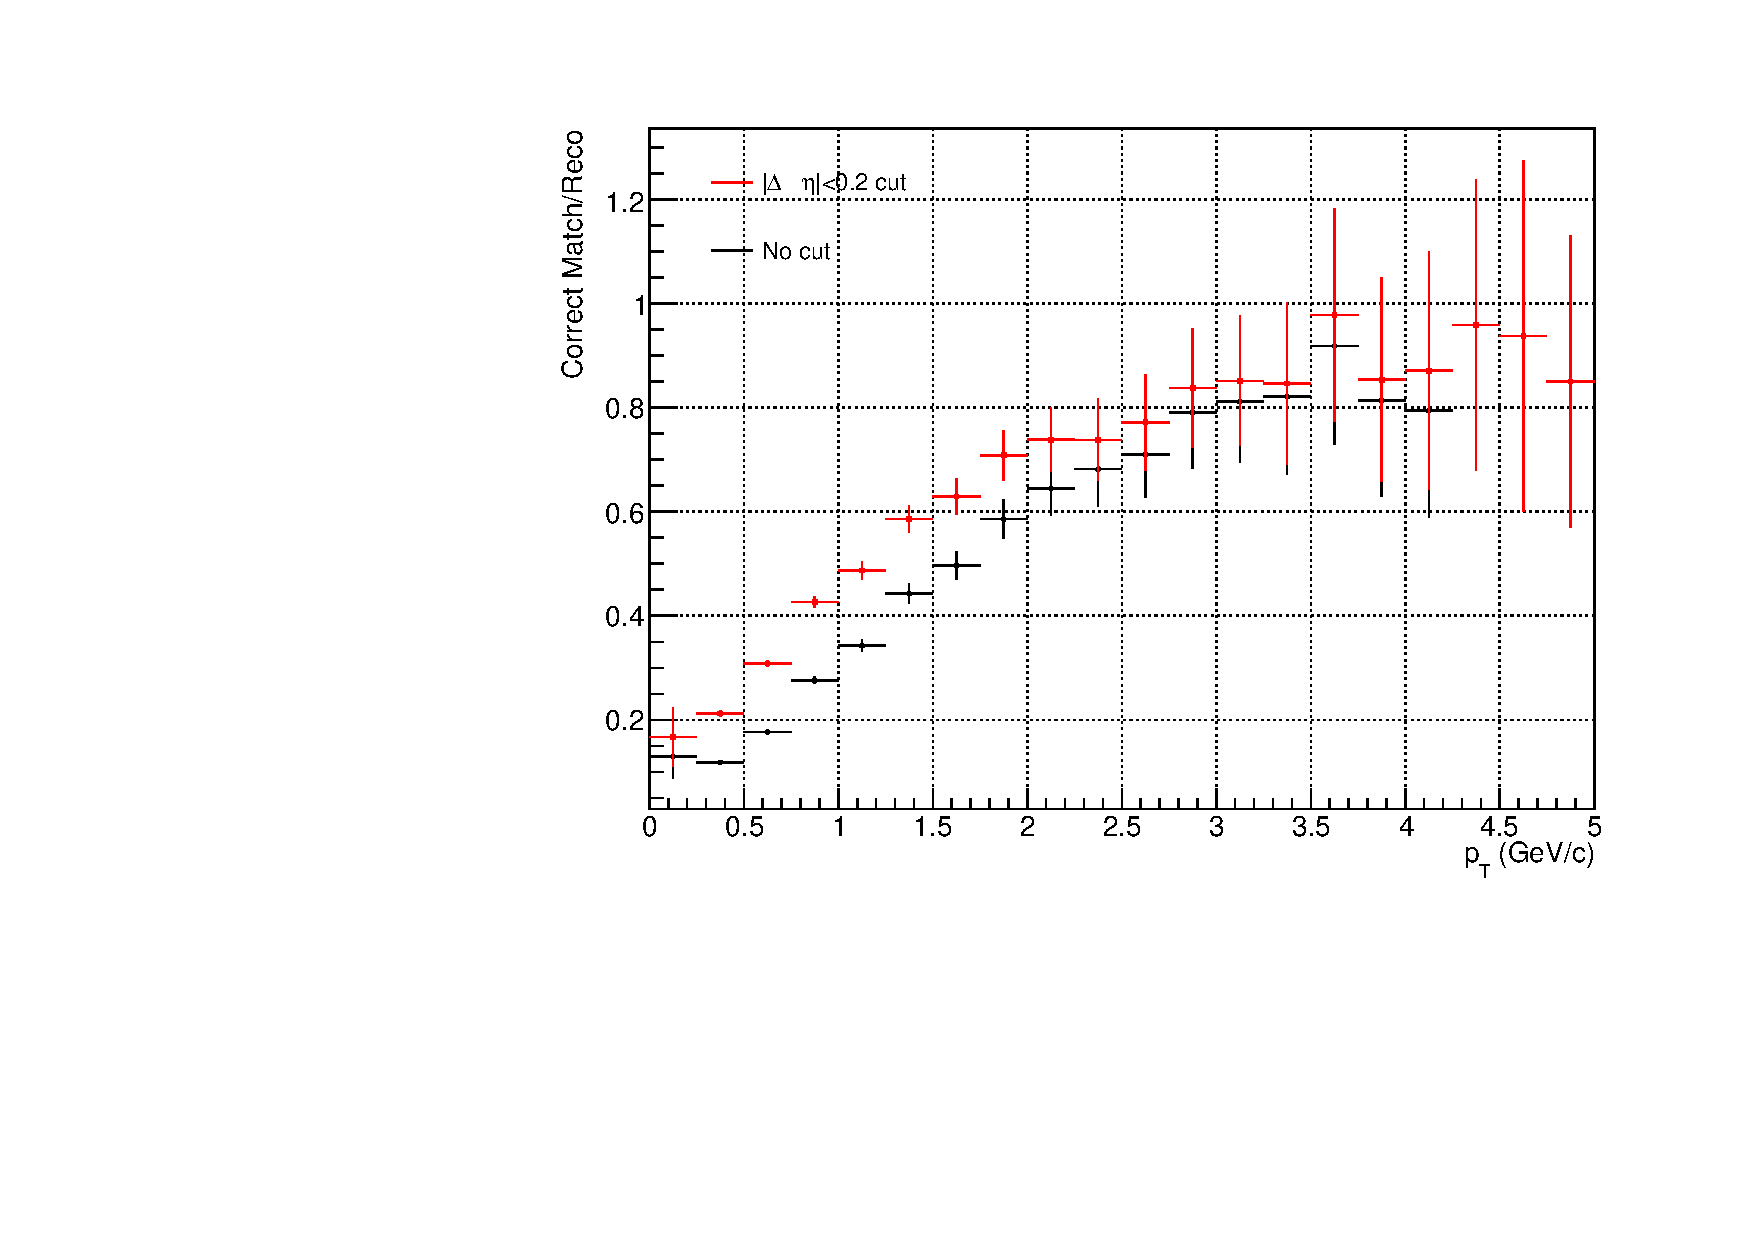
\includegraphics[width=\textwidth]{fig/3_5_6_purity_pt.pdf}
                    \caption{Purity of $p_T$}
                    \label{purity_of_pt}
                \end{minipage}
                \hfill
                \begin{minipage}{0.45\textwidth}
                    \centering
                    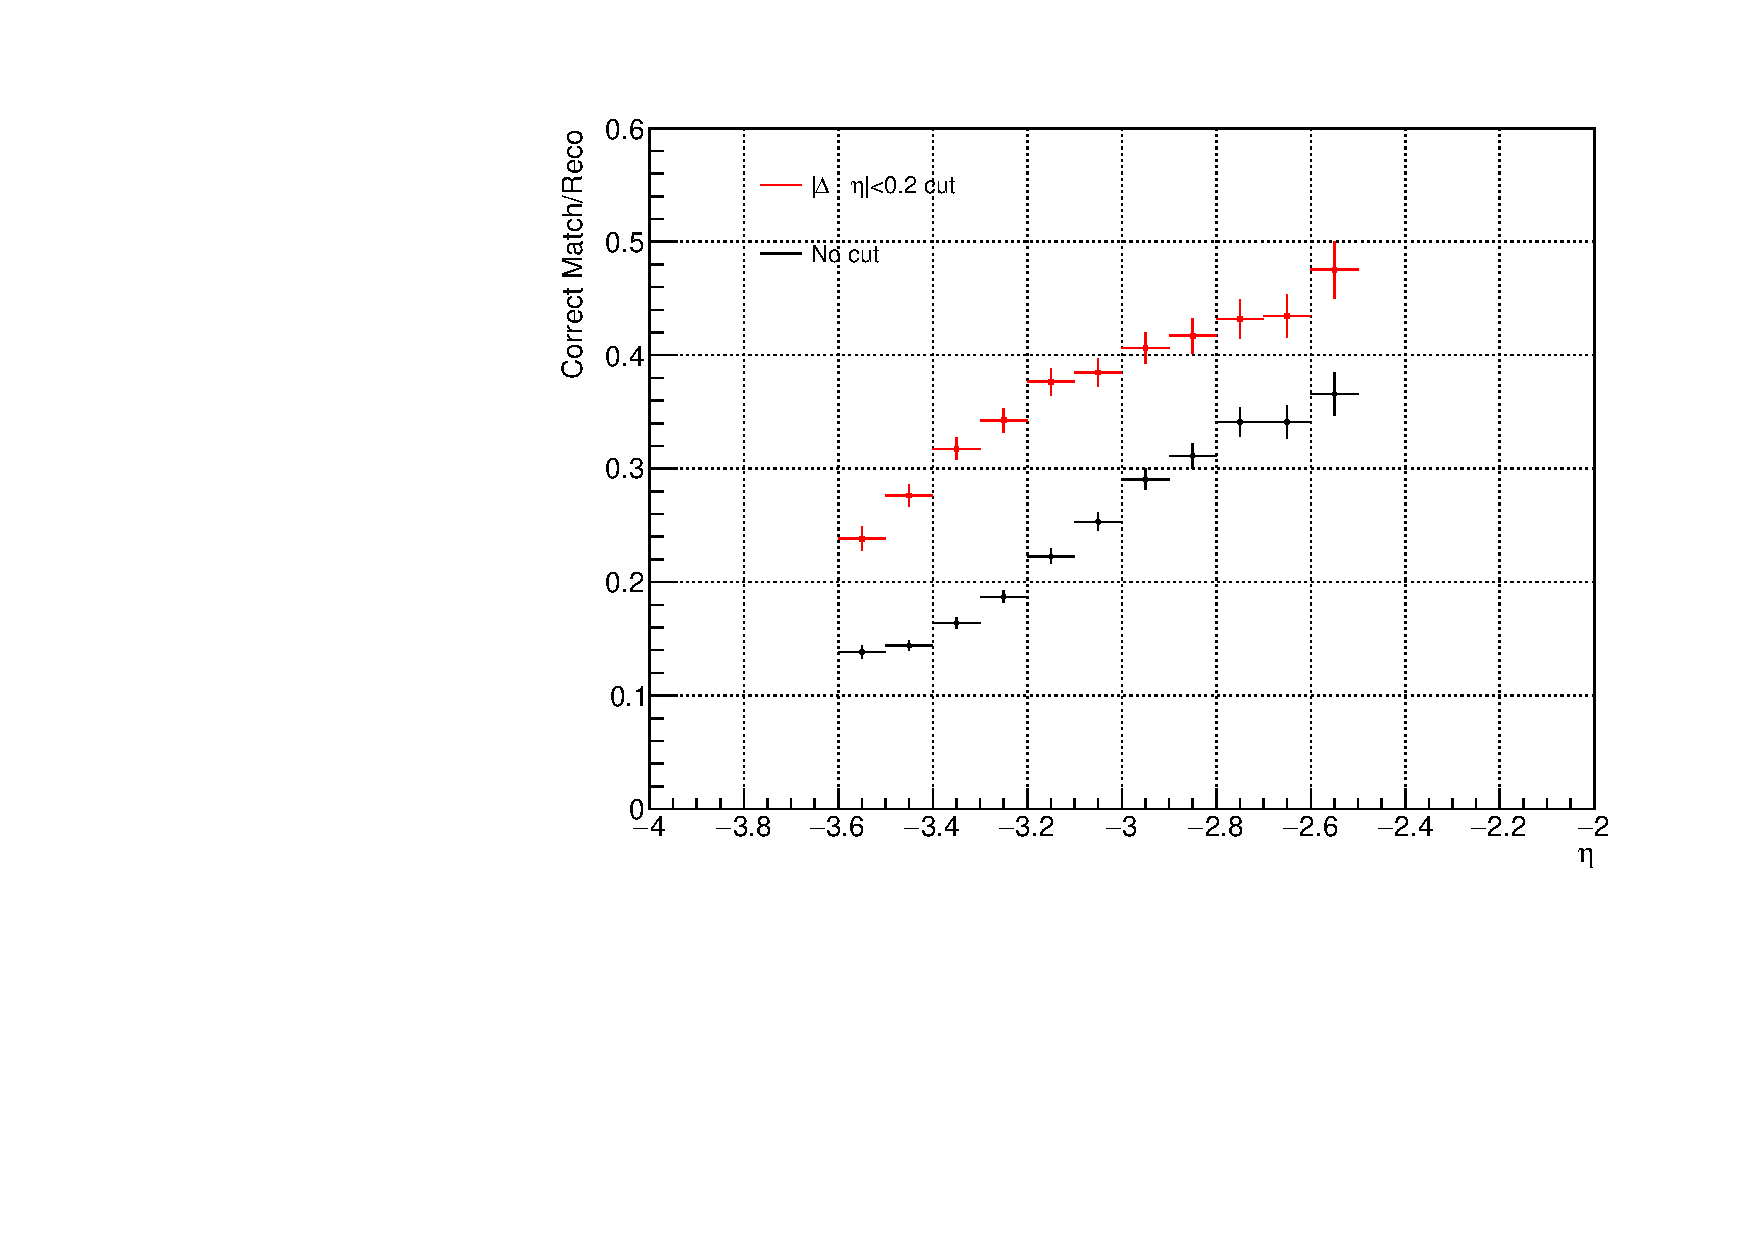
\includegraphics[width=\textwidth]{fig/3_5_6_purity_eta.pdf}
                    \caption{Purity of $\eta$} 
                    \label{purity_of_eta}
                \end{minipage}
                \\
                \vspace{1em}
                \begin{minipage}{0.45\textwidth}
                    \centering
                    \includegraphics[width=\textwidth]{fig/3_5_6_effpuri_pt.pdf}
                    \caption{Efficency $\times$ Purity of $p_T$}
                    \label{EffPuri_of_pt}
                \end{minipage}
                \hfill
                \begin{minipage}{0.45\textwidth}
                    \centering
                    \includegraphics[width=\textwidth]{fig/3_5_6_effpuri_eta.pdf}
                    \caption{Efficency $\times$ Purity of $\eta$}
                    \label{EffPuri_of_eta}
                \end{minipage}
            \end{figure}
            The \( |\Delta \eta| < 0.2 \) cut was applied in such a way as to discard as few correct match tracks as possible while removing fake match tracks. For the \( p_T \) distribution, the efficiency drops below 2 GeV, but the matching purity improves. The product of efficiency \(\times\) purity remains unchanged compared to before the cut. This indicates that the cut does not significantly remove correct matches. For the \(\eta\) distribution, efficiency is reduced in the range \( -3.6 < \eta < -3 \), but matching purity improves in the range \( -4 < \eta < -2 \). Similarly, the product of efficiency \(\times\) purity for \(\eta\) also remains unchanged compared to before the cut.

    %第4章
    \newpage
\clearpage
\section{Results and Discussion}
In this chapter, the graphs of the $\omega$ and $\phi$ yields calculated in \ref{Analysis:Dimuon:Yield:Results} are presented as the conclusion.
    \begin{figure}[htbp]
        \centering
        % Left side figure
        \begin{minipage}{0.45\textwidth} % Specify width using minipage
            \centering
            \includegraphics[width=\textwidth]{fig/4_omega_yield.pdf} % Left side image
            \caption{$\omega$ yield}
            \label{fig:omega_yield}
        \end{minipage}
        % Right side figure
        \hfill
        \begin{minipage}{0.45\textwidth}
            \centering
            \includegraphics[width=\textwidth]{fig/4_phi_yield.pdf} % Right side image
            \caption{$\phi$ yield}
            \label{fig:phi_yield}
        \end{minipage}
    \end{figure}
    Figures \ref{fig:omega_yield} and \ref{fig:phi_yield} show the transverse momentum spectra of the production yields of $\omega$ and $\phi$. The horizontal axis represents the transverse momentum of $\omega$ and $\phi$, while the vertical axis represents the number of counts.  
    Since these spectra are uncorrected, no physical discussion can be made. However, it is observed that the yields decrease as the transverse momentum increases. This behavior is similar to the $p_T$ spectrum of $\phi$ production cross-sections measured using forward dimuons in Run 2. Although the $p_T$ spectrum of $\omega$ production cross-sections has not been published, the present results exhibit a similar trend to those measured in Run 2.  
    Here, it is necessary to consider the contribution of $\rho \rightarrow \mu\mu$. The $\rho$ meson has a mean mass of $m = 775.26$ MeV and a full width of $\Gamma = 149.1$ MeV, leading to a broader distribution than $\omega$, which is located at a very similar mass position. Given that the signal extraction method used in this analysis accounts for the broad width of the $\rho$, it is considered that the peak structure of $\omega$ is not significantly affected.  
    As a future prospect, improving the resolution of single-muon kinematic variables will enhance the mass resolution, making the $\omega$ peak sharper and allowing better separation between the $\rho$ and $\omega$ peaks. Additionally, by applying acceptance-efficiency corrections using the forward detector system for $\omega \rightarrow \mu\mu$ and $\phi \rightarrow \mu\mu$ dimuon reconstruction, the integrated luminosity can be determined from the event counts. This will enable the calculation of production cross-sections from the present results, allowing for direct comparison with Run 2 results.


    Discuss single muon track reconstruction, \ref{matching improvements}, and future prospects as well. In the current muon track reconstruction algorithm, the pseudorapidity (\(\eta\)) and azimuthal angle (\(\phi\)) of the muon are determined using the MFT standalone track to improve their precision. However, the DCA is calculated using parameters obtained from the global fit of the MFT-MCH-MID track. Since using tracks closer to the collision point allows for more precise measurements unaffected by the absorber, it is expected that the accuracy of the DCA measurement can be improved by using the parameters of the MFT track that constitutes the MFT-MCH-MID track.Furthermore, improvements in MFT-MCH matching are also needed. As seen in \ref{purity_of_pt}, the matching purity significantly decreases at low transverse momentum (\( p_T \)). This degradation occurs because low-\( p_T \) muons undergo multiple scattering and energy loss in the absorber, making MFT-MCH matching more challenging. However, this study demonstrated that applying a \( \Delta \eta \) cut improves matching purity in the low-\( p_T \) region. This result suggests that continued analysis can further enhance matching purity.

    The ultimate goal is to measure the changes in the mass distribution of light vector mesons in lead-lead collision events. This study has revealed several remaining challenges, including issues with matching purity at low transverse momentum and the development of the track reconstruction algorithm. Additionally, improving the quality of muon tracks in high-multiplicity events in heavy-ion collisions is another challenge. As a first step, efforts will be focused on improving matching purity and developing the track reconstruction algorithm in proton-proton collisions, where the event multiplicity is relatively low. Subsequently, similar improvements will be pursued in heavy-ion collisions. Ultimately, the aim is to clarify the changes in the mass distribution of light vector mesons due to QGP formation and observe the restoration of chiral symmetry.
\section{Summary}
    In this study, we analyzed forward muon pairs in ALICE from $\sqrt{s} = 13.6$ TeV $pp$ collisions. The peaks corresponding to $\omega \rightarrow \mu\mu$ and $\phi \rightarrow \mu\mu$ in the dimuon mass distribution were extracted by fitting them with Gaussian functions, while other components were fitted with an exponential function. These analyses were performed for each transverse momentum range, and the transverse momentum spectra of $\omega$ and $\phi$ yields were presented. Additionally, an analysis was conducted to improve the matching purity between the MFT, introduced in Run 3, and the downstream detectors. By applying a cut on the difference in $\eta$ between the MFT Track and the MCH Track that constitute the Global Track, we demonstrated the ability to remove Fake Match tracks. Furthermore, the optimal MFT-MCH matching $\chi^2$ cut was determined using the signal yields of $\omega$ and $\phi$. As a future prospect, further improvements in the quality of Single Muon Tracks will be pursued. Ultimately, this study aims to clarify the changes in the mass distribution of light vector mesons caused by the formation of the QGP in lead-lead nuclear collisions.

    \newpage
    \begin{thebibliography}{99}
      %\cite{ParticleDataGroup:2024cfk}
\bibitem{ParticleDataGroup:2024cfk}
S.~Navas \textit{et al.} [Particle Data Group],
%``Review of particle physics,''
Phys. Rev. D \textbf{110}, no.3, 030001 (2024)
doi:10.1103/PhysRevD.110.030001
%771 citations counted in INSPIRE as of 17 Jan 2025
%http://cds.cern.ch/record/2907603
%\cite{Weise:1993ax}
\bibitem{Weise:1993ax}
W.~Weise,
%``Nuclear aspects of chiral symmetry,''
Nucl. Phys. A \textbf{553}, 59C-72C (1993)
doi:10.1016/0375-9474(93)90615-5
%40 citations counted in INSPIRE as of 17 Jan 2025
%https://www.sciencedirect.com/science/article/pii/0375947493906155?via%3Dihub
\bibitem{QCDPhaseDiagram}
%\bibitem{Maire:2025215}
A. Maire, "Phase diagram of QCD matter: Quark-Gluon Plasma," 2015. Available at: https://cds.cern.ch/record/2025215

\bibitem{QGP_evo}
ALICE Collaboration., Acharya, S., Adamová, D. et al. The ALICE experiment: a journey through QCD. Eur. Phys. J. C 84, 813 (2024). https://doi.org/10.1140/epjc/s10052-024-12935-y
%\cite{Geurts:2022xmk}
\bibitem{Geurts:2022xmk}
%F.~Geurts and R.~A.~Tripolt,
%``Electromagnetic probes: Theory and experiment,''
%Prog. Part. Nucl. Phys. \textbf{128}, 104004 (2023)
%doi:10.1016/j.ppnp.2022.104004
%[arXiv:2210.01622 [hep-ph]].
%25 citations counted in INSPIRE as of 17 Jan 2025

F. Geurts and R. A. Tripolt, Prog. Part. Nucl. Phys. 128, 104004 (2023) doi:10.1016/j.ppnp.2022.104004
%\cite{ALICE:2023jef}
\bibitem{ALICE:2023jef}
%S.~Acharya\textit{et al.} [ALICE],
%``Dielectron production in central Pb$-$Pb collisions at $\sqrt{s_\mathrm{NN}}$ = 5.02 TeV,''
%[arXiv:2308.16704 [nucl-ex]].
%15 citations counted in INSPIRE as of 17 Jan 2025
S. Acharya et al. [ALICE Collaboration], Eur. Phys. J. C 84, 813 (2024) doi:10.1140/epjc/s10052-024-12935-y
%\cite{Rapp:1999ej}
\bibitem{Rapp:1999ej}
R.~Rapp and J.~Wambach,
%``Chiral symmetry restoration and dileptons in relativistic heavy ion collisions,''
Adv. Nucl. Phys. \textbf{25}, 1 (2000)
doi:10.1007/0-306-47101-9\_1
[arXiv:hep-ph/9909229 [hep-ph]].
%905 citations counted in INSPIRE as of 17 Jan 2025
%https://inspirehep.net/literature/506479

%\cite{NA60:2007cjy}
\bibitem{NA60}
S.~Damjanovic \textit{et al.} [NA60],
%``NA60 results on the rho spectral function in In-In collisions,''
Nucl. Phys. A \textbf{783}, 327-334 (2007)
doi:10.1016/j.nuclphysa.2006.11.015
[arXiv:nucl-ex/0701015 [nucl-ex]].
%107 citations counted in INSPIRE as of 17 Jan 2025
\bibitem{MFT_TDR}
%\bibitem{CERN-LHCC-2015-001}
"Technical Design Report for the Muon Forward Tracker," CERN-LHCC-2015-001, ALICE-TDR-018, 2015. Available at

    \end{thebibliography}
   % \input{5_appendix.tex}
\end{document}